% !TeX program = lualatex
% !TeX encoding = utf8
% !TeX spellcheck = english
% !TeX version = 2020
%
% **************************************************
% Document Class Definition
% **************************************************
% B5->9pt
\documentclass[%
    paper=A4,               % paper size --> A4 is default in Germany
    twoside=false,          % onesite or twoside printing TODO: true
    openright,              % doublepage cleaning ends up right side
    parskip=half,           % spacing value / method for paragraphs
    chapterprefix=true,     % prefix for chapter marks
    11pt,                   % font size
    headings=normal,        % size of headings
    bibliography=totoc,     % include bib in toc
    listof=totoc,           % include listof entries in toc
    titlepage=on,           % own page for each title page
    captions=tableabove,    % display table captions above the float env
    chapterprefix=false,    % do not display a prefix for chapters
    appendixprefix=false,   % but display a prefix for appendix chapter
    draft=false,            % value for draft version
]{scrreprt}%
%
%
% **************************************************
% Setup YOUR thesis document in this file !
% **************************************************
% !TEX root = thesis.tex
%
\usepackage{iftex}
% **************************************************
% Files' Character Encoding
% **************************************************
\ifPDFTeX
    \usepackage[utf8]{inputenc}
\fi
%
% **************************************************
% Information and Commands for Reuse
% **************************************************
\newcommand{\thesisTitle}{Nerve Fiber Modelling and 3D-PLI Simulations:\\ A Fiber Architect Simulation Toolbox}
\newcommand{\thesisName}{Felix Matuschke}
\newcommand{\thesisSubject}{Documentation}
\newcommand{\thesisDate}{\today}
\newcommand{\thesisVersion}{My First Draft}
%
\newcommand{\thesisFirstReviewer}{Prof. Dr. Gunnar Schr\"{o}der}
\newcommand{\thesisFirstReviewerUniversity}{\protect{IBI-7}}
\newcommand{\thesisFirstReviewerDepartment}{Forschungszentrum J\"{u}lich}
%
\newcommand{\thesisSecondReviewer}{Prof. Dr. Katrin Amunts}
\newcommand{\thesisSecondReviewerUniversity}{\protect{INM-1}}
\newcommand{\thesisSecondReviewerDepartment}{Forschungszentrum J\"{u}lich}
%
\newcommand{\thesisFirstSupervisor}{Prof. Dr. Markus Axer}
\newcommand{\thesisFirstSupervisorUniversity}{\protect{INM-1}}
\newcommand{\thesisFirstSupervisorDepartment}{Forschungszentrum J\"{u}lich}
%
\newcommand{\thesisUniversity}{\protect{Heinrich-Heine-Universit\"{a}t D\"{u}sseldorf}}
\newcommand{\thesisUniversityDepartment}{Math.-Nat. Fakult\"{a}t}
\newcommand{\thesisUniversityInstitute}{}
\newcommand{\thesisUniversityGroup}{}
\newcommand{\thesisUniversityCity}{D\"{u}sseldorf}
\newcommand{\thesisUniversityStreetAddress}{Universitt\"{a}sstra{\ss}e 1}
\newcommand{\thesisUniversityPostalCode}{40225 D\"{u}sseldorf}
%
\newcommand{\thesisInstitute}{\protect{Forschungszentrum J\"{u}lich}}
\newcommand{\thesisInstituteDepartment}{Institut für Neurowissenschaften und Medizin}
\newcommand{\thesisInstituteInstitute}{Strukturelle und funktionelle Organisation des Gehirns (INM-1)}
\newcommand{\thesisInstituteGroup}{Faserbahnarchitektur}
\newcommand{\thesisInstituteCity}{J\"{u}lich}
\newcommand{\thesisInstituteStreetAddress}{Wilhelm-Johnen-Stra{\ss}e}
\newcommand{\thesisInstitutePostalCode}{52428 J\"{u}lich}
%
% **************************************************
% Debug LaTeX Information
% **************************************************
\usepackage{silence}
% \WarningFilter[references]{latex} {There were undefined references}
\WarningFilter[references]{latex}{Reference}
\WarningFilter[citations]{latex}{Citation}
% \listfiles
%
% **************************************************
% User Commands
% **************************************************
%
% \makeatletter
% \renewcommand\listoftables{%
%         \@starttoc{lot}%
% }
% \makeatother
% %
% \makeatletter
% \renewcommand\listoffigures{%
%         \@starttoc{lof}%
% }
% \makeatother
% %
% \makeatletter
% \renewcommand\lstlistoflistings{%
%         \@starttoc{lof}%
% }
% \makeatother
%
%
% **************************************************
% Pre cleanthesis imports
% **************************************************
\RequirePackage[dvipsnames]{xcolor}
\usepackage{tikz}
%
% **************************************************
% Load and Configure Packages
% **************************************************
\usepackage[english]{babel} % babel system, adjust the language of the content
\PassOptionsToPackage{% setup clean thesis style
    figuresep=colon,%
    hangfigurecaption=false,%
    hangsection=true,%
    hangsubsection=true,%
    sansserif=true,%
    configurelistings=true,%
    colorize=full,%
    colortheme=bluemagenta,%
    configurebiblatex=true,%
    bibsys=biber,%
    bibfile=bib-refs,%
    bibstyle=alphabetic,%
    bibsorting=nty,%
}{cleanthesis}
\usepackage{cleanthesis}
%
% \colorlet{citeColor}{green!50!black}
% \colorlet{linkColor}{green!75!black>wheel,1,2}
% \colorlet{urlColor}{green!75!black>twheel,1,2}
\colorlet{citeColor}{violet>twheel,2,3}
\colorlet{linkColor}{violet}
\colorlet{urlColor}{violet>twheel,1,3}
%
\hypersetup{% setup the hyperref-package options
    pdftitle={\thesisTitle},    %   - title (PDF meta)
    pdfsubject={\thesisSubject},%   - subject (PDF meta)
    pdfauthor={\thesisName},    %   - author (PDF meta)
    plainpages=false,           %   -
    colorlinks=true,            %   - colorize links?
    pdfborder={0 0 0},          %   -
    breaklinks=true,            %   - allow line break inside links
    bookmarksnumbered=true,     %
    bookmarksopen=true,         %
    citecolor=citeColor,        %
    linkcolor=linkColor,        %
    urlcolor=urlColor,          %
}
%
% **************************************************
%  Packages
% **************************************************
\usepackage{scrhack}
\usepackage{float}              % [H]
\usepackage{graphicx}           % (pdf, png, jpg, eps)
\usepackage[export]{adjustbox}
\usepackage{pdfpages}
\usepackage{subcaption}
\usepackage{minitoc}
\usepackage{tcolorbox}
\usepackage{enumitem}
\usepackage{nameref}
\usepackage{relsize}
%
\newcommand{\subcaptiontab}[2]{%
\multicolumn{1}{l}{%
\begin{minipage}[t]{#1}
\leavevmode\subcaption{#2}
\end{minipage}}
}
\captionsetup{subrefformat=parens}
%
\usepackage{amsmath, amssymb, amsthm, mathtools}
\ifPDFTeX
    % \usepackage{newtxsf} ???
    \usepackage{newtxmath} % new math fonts\usepackage[libertine, vvarbb]{newtxmath}
\else
    \usepackage{fontspec}
    \usepackage[warnings-off={mathtools-colon,mathtools-overbracket}]{unicode-math}
    \usepackage{lualatex-math}
    \setmathfont{Latin Modern Math}
\fi
%
\usepackage{dirtree}
\usepackage[bottom]{footmisc}
%
\usepackage{siunitx}
\usepackage{upgreek}
\sisetup{%
        detect-mode=true,detect-family=false,
        detect-display-math=false,detect-shape=false,
        list-units=brackets,range-units=brackets,
        list-final-separator = {,},
        list-pair-separator={,},
        % list-pair-separator={\text{~and~}},
        range-phrase = {\text{~to~}},
        math-micro=µ,
        binary-units = true
        } %\mathrm{\mu}} %math-micro=\muup,
\AtBeginDocument{\sisetup{math-rm=\mathrm, text-rm=\sffamily}}
%
% \usepackage{caption}
\usepackage[nameinlink]{cleveref}
% \usepackage{esvect} % see \let\vv\mathbf
%
\usepackage{currfile}
\usepackage{blindtext}
%\usepackage{ifplatform}
\usepackage{mwe}
\usepackage{acro}
\usepackage{dirtytalk}
\usepackage{tabularx}
% \usepackage{stackengine}    % for double sided floats
\usepackage{pdflscape}
\usepackage{rotating}        
\newsavebox{\largestimage}   
\newsavebox{\newtable}
%
\acsetup{barriers/use=true,barriers/reset = true}
%
% \crefname{figure}{fig.}{fig.}
% \Crefname{figure}{Fig.}{Fig.}
%
\makeatletter
\def\convertto#1#2{\strip@pt\dimexpr #2*65536/\number\dimexpr 1#1}
\makeatother
%
% \newcommand{\fakechapter}[1]{%
%   \par\refstepcounter{chapter}% Increase section counter
%   \sectionmark{#1}% Add section mark (header)
%   \addcontentsline{toc}{section}{\protect\numberline{\thesection}#1}% Add section to ToC
% %   Add more content here, if needed.
% }
% %
% \newcommand{\fakesection}[1]{%
%   \par\refstepcounter{section}% Increase section counter
%   \sectionmark{#1}% Add section mark (header)
%   \addcontentsline{toc}{section}{\protect\numberline{\thesection}#1}% Add section to ToC
%   % Add more content here, if needed.
% }
%
% **************************************************
%  Minitoc
% **************************************************
\renewcommand*{\partheadstartvskip}{%
  \null\vskip20pt
}
\renewcommand*{\partheadendvskip}{%
  \vskip2pt
}
\renewcommand\beforeparttoc{}
\let\oldparttoc\parttoc
\renewcommand*{\parttoc}{{\hypersetup{hidelinks}\oldparttoc}}
%
% **************************************************
%  Math
% **************************************************
% \AtBeginDocument{\renewcommand{\minus}{\scalebox{0.75}[1.0]{$-$}}} % different height than -
\AtBeginDocument{\renewcommand{\vec}[1]{\mathbf{#1}}}
\newcommand{\mat}[1]{\mathcal{#1}}
\newcommand{\topbar}[1]{\mkern 1.5mu\overline{\mkern-1.5mu#1\mkern-1.5mu}\mkern 1.5mu}
% \usepackage{MnSymbol} defines to many math symbols for pdflatex
\DeclarePairedDelimiter\abs{\lvert}{\rvert}
\DeclarePairedDelimiter\norm{\lVert}{\rVert}
\DeclarePairedDelimiter\ceil{\lceil}{\rceil}
\DeclarePairedDelimiter\floor{\lfloor}{\rfloor}
\DeclareMathOperator{\atantwo}{atan2}
\DeclareMathOperator{\divergence}{div}
\DeclareMathOperator{\gauss}{normal}
\DeclareMathOperator{\mean}{mean}
\DeclareMathOperator{\median}{median}
\DeclareMathOperator{\std}{std}
\DeclareMathOperator{\integer}{int}
\DeclareMathOperator{\round}{round}
%
% **************************************************
% Syntax Highlighting
% **************************************************
\usepackage{listings}
%
\newfloat{lstfloat}{htbp}{lop}
\floatname{lstfloat}{Alg.}
\crefname{lstfloat}{alg.}{alg.}
\Crefname{lstfloat}{Alg.}{Alg.}
\crefname{pluralequation}{eqs.}{eqs.}
\renewcommand{\lstlistingname}{Alg.}
\renewcommand{\lstlistlistingname}{List of Algorithm}
%
\definecolor{syntax_red}{RGB}{160,0,0}
\definecolor{syntax_green}{RGB}{0,160,0}
\definecolor{syntax_blue}{RGB}{0,0,210}
\definecolor{syntax_mauve}{RGB}{150,0,210}
\definecolor{syntax_keywords}{RGB}{255,0,90}
\definecolor{syntax_comments}{RGB}{0,0,113}
%
%
\lstdefinestyle{common}{%
    basicstyle=\footnotesize\ttfamily,
    showstringspaces=false,
    breaklines=false,
    captionpos=b,
    frame=tb,
    xleftmargin=\parindent,
}
%
\lstdefinestyle{cpp}{%
    language=C++,
    style=common,
    keywordstyle=\color{syntax_blue},
    commentstyle=\color{syntax_green},
    stringstyle=\color{syntax_red},
    % identifierstyle=\color{syntax_mauve},
    tabsize=2,
}
% 
\lstdefinestyle{python}{%
    language=Python,
    style=common,
    keywordstyle=\color{syntax_blue},
    commentstyle=\color{syntax_green},
    stringstyle=\color{syntax_red},
    % identifierstyle=\color{syntax_green},
    % procnamekeys={def,class},
	tabsize=3,
}
%
% Hyphenate code
\usepackage[htt]{hyphenat}
%
\newcommand{\breakingperiod}{%
  \penalty0 % allow a break before the period
  .\nobreak\hspace{0pt}%
}
%
\ExplSyntaxOn
%
\NewDocumentCommand{\code}{m}
 {%
  \texttt
   {%
    \seq_set_split:Nnn \l_michael_lw_seq { . } { #1 }
    \seq_use:Nn \l_michael_lw_seq { \breakingperiod }
   }
 }
%
\ExplSyntaxOff
%
% **************************************************
% Tikz & PGFplots
% **************************************************
\usepackage{shellesc}
% \usepackage{tikz} before hyperref
\usepackage{tikz-3dplot}
\usetikzlibrary{math}
\usetikzlibrary{shapes, arrows}
\usetikzlibrary{mindmap, backgrounds}
\usetikzlibrary{calc}
\usetikzlibrary{intersections}
\usetikzlibrary{perspective}
\usetikzlibrary{3d}
\usetikzlibrary{arrows.meta}
\usetikzlibrary{patterns}
\usetikzlibrary{bending} % bend arrow heads
\usetikzlibrary{decorations.pathreplacing}
\usetikzlibrary{positioning}
\usetikzlibrary{quotes,angles}
\tikzset{>=latex}
%
% \usepackage{pdftexcmds} % for hased externalized names
% \makeatletter
% \ifx\pdf@filemdfivesum\undefined\def\pdf@filemdfivesum#{\mdfivesum file}\fi
% \let\filesum\pdf@filemdfivesum
% \makeatother
%
\usepackage{pgfplots}
\pgfplotsset{compat=1.17}
\usepgfplotslibrary{polar}
\usepgfplotslibrary{colorbrewer}
\usepgfplotslibrary{statistics}
\usepgfplotslibrary{groupplots}
\usepgfplotslibrary{patchplots}
\usepgfplotslibrary{colormaps}
\usepgfplotslibrary{fillbetween}
\usepackage{booktabs,colortbl}
\usepackage{multirow}
%
% 3d canvis
\makeatletter
\tikzoption{canvas is plane}[]{\@setOxy#1}
\def\@setOxy O(#1,#2,#3)x(#4,#5,#6)y(#7,#8,#9)%
  {\def\tikz@plane@origin{\pgfpointxyz{#1}{#2}{#3}}%
   \def\tikz@plane@x{\pgfpointxyz{#4}{#5}{#6}}%
   \def\tikz@plane@y{\pgfpointxyz{#7}{#8}{#9}}%
   \tikz@canvas@is@plane
  }
\makeatother
%
\newlength{\tikzwidth}
\newlength{\tikzheight}
\setlength{\tikzwidth}{\textwidth} %13.87303cm
\setlength{\tikzheight}{\textheight} %22.37076cm
%
\makeatletter
\newcommand{\inputtikz}[1]{%
    \input{#1.tikz}
}
\makeatother
% \makeatletter
% \newcommand{\inputtikz}[2][false]{%
%     \ifthenelse{\boolean{#1}}{%
%         \input{#2.tikz}
%     }{%
% 	\IfFileExists{tikz/#2.pdf}{% check if pdf tikz/.../*.pdf exists
% 		\includegraphics{tikz/#2.pdf}
% 	}{ % build ext tikz
% 		\input{#2.tikz}
% 	}}
% }
% \makeatother
% 
\makeatletter
% 
\tikzdeclarecoordinatesystem{rel}{%
    \tikzset{cs/.cd,x=0pt,y=0pt,#1}%
    \pgfpointlineattime{(\tikz@cs@x)}%
       {\pgfpointanchor{\tikz@pp@name{\tikz@cs@node}}{south west}}%
       {\pgfpointanchor{\tikz@pp@name{\tikz@cs@node}}{south east}}%
    \edef\tikz@cs@x{\the\pgf@x}%
    \pgfpointlineattime{(\tikz@cs@y)}%
       {\pgfpointanchor{\tikz@pp@name{\tikz@cs@node}}{south west}}%
       {\pgfpointanchor{\tikz@pp@name{\tikz@cs@node}}{north west}}%
    \pgfpoint{\tikz@cs@x}{\pgf@y}%
  }
% 
% % Hook into Tikz coordinate parse to provide (<name>:<rel x>x<rel y>)
% \def\tikz@parse@relcs#1(#2:#3,#4){%
% \tikz@parse@coordinatesystem#1(rel cs:name={#2},x={#3},y={#4})%
% }
% \let\tikz@parse@relcs@polar@saved=\tikz@parse@polar
% \def\tikz@parse@polar#1(#2:#3){%
%   \pgfutil@in@{,}{#3}%
%   \ifpgfutil@in@%
%     \let\@next\tikz@parse@relcs%
%   \else%
%     \let\@next\tikz@parse@relcs@polar@saved%
%   \fi%
%   \@next#1(#2:#3)%
% }

\makeatother
% 
%
\usepackage{environ}
\makeatletter
\def\forcetikzscale{false}
\newsavebox{\measure@tikzpicture}
\NewEnviron{tikzsize}[2]{% use false for non externalized images
    \pgfmathsetmacro{\tikzscale}{1}
	\ifthenelse{\boolean{\forcetikzscale}}{%
	    \tikzset{external/export=false,external/optimize=false}% force translation of this BODY (and do not optimize it away as it would usually do):
	    \begin{lrbox}{\measure@tikzpicture}%
		\BODY
		\end{lrbox}%
		\expandafter\pgfmathparse{#1/\wd\measure@tikzpicture}%
		\edef\tikzscalewidth{\pgfmathresult}%
		\expandafter\pgfmathparse{#2/\ht\measure@tikzpicture}%
		\edef\tikzscaleheight{\pgfmathresult}%
		\pgfmathparse{min(\tikzscalewidth, \tikzscaleheight)}%
		\edef\tikzscale{\pgfmathresult}%
		\BODY
	}{%
	\tikzifexternalizingnext{%
		\begin{lrbox}{\measure@tikzpicture}%
		\tikzset{external/export next=false,external/optimize=false}% force translation of this BODY (and do not optimize it away as it would usually do):
		\BODY
		\end{lrbox}%
		\expandafter\pgfmathparse{#1/\wd\measure@tikzpicture}%
		\edef\tikzscalewidth{\pgfmathresult}%
		\expandafter\pgfmathparse{#2/\ht\measure@tikzpicture}%
		\edef\tikzscaleheight{\pgfmathresult}%
		\pgfmathparse{min(\tikzscalewidth, \tikzscaleheight)}%
		\edef\tikzscale{\pgfmathresult}%
		\BODY
    }{% this will re-use an existing external graphics:
		\BODY
	}
	}
}
\makeatother
%
% **************************************************
% PGFplotsTable
% **************************************************
\usepackage{pgfplotstable}
\usepackage{array,multirow,makecell}
\newcolumntype{R}[1]{>{\raggedleft\arraybackslash}b{#1}}
\newcolumntype{L}[1]{>{\raggedright\arraybackslash}b{#1}}
\newcolumntype{C}[1]{>{\centering\arraybackslash}b{#1}}
% \newcolumntype{RP}[1]{>{\raggedleft\arraybackslash}p{#1}}
% \newcolumntype{LP}[1]{>{\raggedright\arraybackslash}p{#1}}
% \newcolumntype{CP}[1]{>{\centering\arraybackslash}p{#1}}
\newcolumntype{A}[1]{>{\raggedleft\arraybackslash}m{#1}}
\newcolumntype{B}[1]{>{\raggedright\arraybackslash}m{#1}}
\newcolumntype{M}[1]{>{\centering\arraybackslash}m{#1}}
%
% \captionsetup[table]{textfont=it, parskip=10em} % skip does not work for table
\pgfplotstableset{thesisTableStyle/.style={%
    every even row/.style={before row={\rowcolor[gray]{0.90}}},
    % empty cells with={--}, % replace empty cells with '--'
    every head row/.style={before row=\toprule,after row=\midrule},
    every last row/.style={after row=\bottomrule},
}}
%
\pgfplotstableset{%
    rowbf/.style={%
        postproc cell content/.append code={%
          \count0=\pgfplotstablerow
            \advance\count0 by1
            \ifnum\count0=#1
              \pgfkeysalso{@cell content=\textbf{##1}}%
            \fi
        },
    },
}
\pgfplotstableset{%
    rowem/.style={%
        postproc cell content/.append code={%
          \count0=\pgfplotstablerow
            \advance\count0 by1
            \ifnum\count0=#1
              \pgfkeysalso{@cell content=\emph{##1}}%
            \fi
        },
    },
}
%
% every row 3 column 3/.style={postproc cell content/.style=
%         {@cell content=\textbf{##1}}}
%
% **************************************************
% User Macros
% **************************************************
\newcommand{\tu}{\textunderscore}
% \newcommand{\tu}{\textscale{.7}{\textunderscore}}
% \newcommand{\tum}{\textscale{.7}{\_}}
\newcommand{\note}[1]{\textcolor{gray}{\textit{#1}}}
\newcommand{\dummy}{\textcolor{blue!75!white}{\textbf{\{...\}}}}
\newcommand{\todo}[1]{\textcolor{blue!75!white}{\textbf{\{#1\}}}}
\newcommand{\TODO}[1]{\textcolor{red!75!white}{\textbf{\{#1\}}}}
% 
% **************************************************
% Debug LaTeX Information
% **************************************************
% \usepackage{showframe}
%
% **************************************************
% Custom Colors
% **************************************************
%  from colorbrewer
\pgfplotsset{cycle list/Dark2}
%
% \definecolor{set11}{HTML}{e41a1c}
% \definecolor{set12}{HTML}{377eb8}
% \definecolor{set13}{HTML}{4daf4a}
% \definecolor{set14}{HTML}{984ea3}
% \definecolor{set15}{HTML}{ff7f00}
% \definecolor{set16}{HTML}{ffff33}
% \definecolor{set17}{HTML}{a65628}
% \definecolor{set18}{HTML}{f781bf}
% %
% \definecolor{set21}{HTML}{66c2a5}
% \definecolor{set22}{HTML}{fc8d62}
% \definecolor{set23}{HTML}{8da0cb}
% \definecolor{set24}{HTML}{e78ac3}
% \definecolor{set25}{HTML}{a6d854}
% \definecolor{set26}{HTML}{ffd92f}
% \definecolor{set27}{HTML}{e5c494}
% \definecolor{set28}{HTML}{b3b3b3}
%
\definecolor{dark21}{HTML}{1b9e77}
\definecolor{dark22}{HTML}{d95f02}
\definecolor{dark23}{HTML}{7570b3}
\definecolor{dark24}{HTML}{e7298a}
\definecolor{dark25}{HTML}{66a61e}
\definecolor{dark26}{HTML}{e6ab02}
\definecolor{dark27}{HTML}{a6761d}
\definecolor{dark28}{HTML}{666666}
%
% \colorlet{sred}{set11}
% \colorlet{sgreen}{set13}
% \colorlet{sblue}{set12}
% %
% \colorlet{dred}{dark22}
% \colorlet{dgreen}{dark21}
% \colorlet{dblue}{dark23}
%
\colorlet{RED}{dark22}
\colorlet{GREEN}{dark21}
\colorlet{BLUE}{dark23}
%
% \makeatletter
% \definecolor{cc21}{HTML}{A6CEE3}
% \definecolor{cc22}{HTML}{1F78B4}
% \pgfplotscreateplotcyclelist{cc2}{cc21, cc22}
% \makeatother
%
\pgfplotsset{%
  colormap/cividis/.style={colormap={cividis}{[1pt]
    rgb(0pt)=(0.00000000, 0.13511200, 0.30475100);
    rgb(25pt)=(0.25974000, 0.30512000, 0.42281000);
    rgb(50pt)=(0.48514100, 0.48245100, 0.47038400);
    rgb(75pt)=(0.73242200, 0.67736400, 0.42571700);
    rgb(100pt)=(0.99573700, 0.90934400, 0.21777200);
}},
  colormap/twilight/.style={colormap={twilight}{[1pt]
    rgb(0pt)=(0.8857501584075443, 0.8500092494306783, 0.8879736506427196);
    rgb(25pt)=(0.38407269378943537, 0.46139018782416635, 0.7309466543290268);
    rgb(50pt)=(0.18488035509396164, 0.07942573027972388, 0.21307651648984993);
    rgb(75pt)=(0.6980608153581771, 0.3382897632604862, 0.3220747885521809);
    rgb(100pt)=(0.8857115512284565, 0.8500218611585632, 0.8857253899008712);
}}}
%   colormap/twilight_shifted/.style={colormap={twilight_shifted}{[1pt]
%     rgb(0pt)=(0.18739228342697645, 0.07710209689958833, 0.21618875376309582);
%     rgb(25pt)=(0.38407269378943537, 0.46139018782416635, 0.7309466543290268);
%     rgb(50pt)=(0.8857115512284565, 0.8500218611585632, 0.8857253899008712);
%     rgb(75pt)=(0.6980608153581771, 0.3382897632604862, 0.3220747885521809);
%     rgb(100pt)=(0.18488035509396164, 0.07942573027972388, 0.21307651648984993);
% }}}
%
\setcounter{secnumdepth}{3}
\setcounter{minitocdepth}{4}
\mtcsetoffset{minitoc}{-4em}
\Urlmuskip=0mu plus 1mu
\AfterEndEnvironment{figure}{\noindent\ignorespaces}
%
%\ifshellescape
\usetikzlibrary{external}
\tikzexternalize[%
    optimize command away=\includepdf,
    prefix=tikz/,
    figure name=\thesubsection-,
    % mode=list and make,
    ]
%
% \def\forcetikzscale{true}
% \tikzset{external/force remake}
% 
% \includeonly{%
% content/titlepages,
% content/abstract,
% content/acknowledgment,
% content/01-chapter-introduction,
% content/02-chapter-neuroanatomy,
% content/03-chapter-theory,
% content/04-chapter-software-model,
% content/05-chapter-software-simulation,
% content/06-chapter-software,
% content/07-chapter-analysis-model,
% content/08-chapter-analysis-simulation,
% content/09-chapter-conclusion,
% content/declaration
% content/appendix,
% }
% 
% 
%%%%%%%%%%%%%%%%%%%%%%%%%%%
% Official Acronyms
%%%%%%%%%%%%%%%%%%%%%%%%%%%
\DeclareAcronym{3D-PLI}{short = 3D-PLI, long = 3D-Polarized Light Imaging}
\DeclareAcronym{AABB}{short = AABB, long = axis aligned bounding box}
\DeclareAcronym{API}{short = API, long = application programming interface}
\DeclareAcronym{CCD}{short = CCD, long = charge-coupled device}
\DeclareAcronym{CC}{short = CC, long = conical capsule}
\DeclareAcronym{CEA}{short = CEA, long = Alternative Energies and Atomic Energy Commission}
\DeclareAcronym{CPU}{short = CPU, long = central processing unit}
\DeclareAcronym{GM}{short = GM, long = gray matter}
\DeclareAcronym{GPU}{short = GPU, long = graphics processing unit}
\DeclareAcronym{HBP}{short = HBP, long = Human Brain Project}
\DeclareAcronym{LAP}{short = LAP, long = large area polarimeter}

\DeclareAcronym{LMP}{short = LMP, long = large metripol}
\DeclareAcronym{LMP3D}{short = LMP3D, long = large metripol three dimensional}
\DeclareAcronym{MRI}{short = MRI, long = Magnetic Resonance Imaging}
\DeclareAcronym{PBS}{short = PBS, long = phosphate buffer saline}
\DeclareAcronym{TPFM}{short = TPFM, long = two photon fluorescence microscopy}
\DeclareAcronym{MAGIC}{short = MAGIC, long = Myelin Autofluorescence imaging by Glycerol Induced Contrast enhancement}
% \DeclareAcronym{PM}{short = PM, long = polarization microscop}
\DeclareAcronym{RAM}{short = RAM, long = random access memory}
\DeclareAcronym{VOI}{short = VOI, long = volume of interest}
\DeclareAcronym{WM}{short = WM, long = white matter}
\DeclareAcronym{dMRI}{short = dMRI, long = diffusion MRI}
\DeclareAcronym{fps}{short = fps, long = frames per second}
\DeclareAcronym{FOM}{short = FOM, long = fiber orientation map}
\DeclareAcronym{ROI}{short = ROI, long = region of interest}
\DeclareAcronym{USAF}{short = USAF, long = U. S. Air Force}
\DeclareAcronym{WSL}{short = WSL, long = Windows Subsystem for Linux}
% 
\DeclareAcronym{fastPLI}{short = fastPLI, long = fiber architecture simulation toolbox for 3D-PLI, short-format = \itshape}
\DeclareAcronym{HDF5}{short = HDF5, long = Hierarchical Data Format v5, short-format = \itshape}
\DeclareAcronym{MEDUSA}{short = MEDUSA, long = Microstructure Environment Designer with UnifiedSphere Atoms, short-format = \itshape}
\DeclareAcronym{MPI}{short = MPI, long = Message Passing Interface, short-format = \itshape}
\DeclareAcronym{OpenGL}{short = OpenGL, long = Open Graphics Library, short-format = \itshape}
\DeclareAcronym{OpenMP}{short = OpenMP, long = Open Multi-Processing, short-format = \itshape}
\DeclareAcronym{simPLI}{short = simPLI, long = simulation method for 3D-PLI, short-format = \itshape}
\DeclareAcronym{ROFL}{short = ROFL, long = robust orientation fitting via least squares, short-format = \itshape}
%
% 
%%%%%%%%%%%%%%%%%%%%%%%%%%%
% Helper
%%%%%%%%%%%%%%%%%%%%%%%%%%%
\newcommand{\name}[1]{\textit{#1}}
% \newcommand{\code}[1]{\texttt{#1}}
\newcommand{\pymodule}[1]{\code{#1}}
%
% 
%%%%%%%%%%%%%%%%%%%%%%%%%%%
% Parameter Code
%%%%%%%%%%%%%%%%%%%%%%%%%%%
\newcommand{\voxelsize}{\code{voxel\tu size}}
\newcommand{\stepsize}{\code{step\tu size}}
\newcommand{\voi}{\code{voi}}
\newcommand{\tissue}{\code{tissue}}
\newcommand{\opticalaxis}{\code{optical\tu axis}}
\newcommand{\propertylist}{\code{property\tu list}}
\newcommand{\pixelsize}{\code{pixel\tu size}}

%%%%%%%%%%%%%%%%%%%%%%%%%%%
% Parameter
%%%%%%%%%%%%%%%%%%%%%%%%%%%
\newcommand{\voxels}{\textnormal{$\mathit{v_{s}}$}}
\newcommand{\pixels}{\textnormal{$\mathit{p_{s}}$}}
\newcommand{\steps}{\textnormal{$\mathit{s_{s}}$}}
\newcommand{\model}{\textit{model}}
\newcommand{\micro}{\textit{micro}}
\newcommand{\macro}{\textit{macro}}
\newcommand{\trel}{\textnormal{$t_\mathit{rel}$}}
\newcommand{\absorp}{\textnormal{$\mu$}}
\newcommand{\dn}{\textnormal{$\Delta n$}}
\newcommand{\intensity}{\textnormal{$I$}}
\newcommand{\opticsigma}{\textnormal{$\sigma_{\text{optic}}$}}
\newcommand{\opticgain}{\textnormal{$g$}}
\newcommand{\filterrots}{\code{filter\tu rotations}}
\newcommand{\wavelength}{\textnormal{$\lambda$}}
\newcommand{\acc}{\name{acc}}
% 
% 
%%%%%%%%%%%%%%%%%%%%%%%%%%%
% Modelling
%%%%%%%%%%%%%%%%%%%%%%%%%%%
\newcommand{\fiberRadius}{\textnormal{$r_f$}}
\newcommand{\fiberRadiusMean}{\textnormal{$\overbar{r}_f$}}
% \newcommand{\fiberRadiusMean}{\textnormal{$\langle{r_f}\rangle$}}
\newcommand{\fiberRadiusSig}{\textnormal{$\sigma_{r_f}$}}
\newcommand{\fiberRadiusMu}{\textnormal{$\mu_{r_f}$}}
\newcommand{\segLength}{\textnormal{$\mathit{seg}_{L}$}}
\newcommand{\segRadius}{\textnormal{$\mathit{seg}_{R}$}}
\newcommand{\segLengthFactor}{\textnormal{$\nu_{l}$}}
\newcommand{\segRadiusFactor}{\textnormal{$\nu_{r}$}}
\newcommand{\modelPsi}{\textnormal{$\Psi$}}
\newcommand{\modelOmega}{\textnormal{$\Omega$}}
\newcommand{\modelRot}{\textnormal{$\Theta$}}
\newcommand{\modelInc}{\textnormal{$\alpha_{\mathit{incl}}$}}
% \newcommand{\modelOri}{\textnormal{$\mathit{O}$}}
% 
% 
%%%%%%%%%%%%%%%%%%%%%%%%%%%
% Other
%%%%%%%%%%%%%%%%%%%%%%%%%%% 
\newcommand{\cc}{\name{C}}
\newcommand{\cpp}{\name{C\texttt{++}}}
\newcommand{\ccpp}{\cc/\cpp}
\newcommand{\python}{\name{Python3}}
\newcommand{\vcs}{Volume Collision Solver}
% 
\newcommand{\eg}{e.\,g.}
\newcommand{\ie}{i.\,e.}
\newcommand{\mean}{\mathrm{mean}}
\newcommand{\std}{\mathrm{std}}
% 
\newcommand{\openmp}{\ac{OpenMP}}
\newcommand{\mpi}{\ac{MPI}}
\newcommand{\opengl}{\ac{OpenGL}}
\newcommand{\simpli}{\ac{simPLI}}
\newcommand{\fastpli}{\ac{fastPLI}}
\newcommand{\rofl}{\ac{ROFL}}
\newcommand{\hdf}[1]{\ac{HDF5}}
% 
% 
%%%%%%%%%%%%%%%%%%%%%%%%%%%
% Units
%%%%%%%%%%%%%%%%%%%%%%%%%%%
\DeclareSIUnit{\arbitraryunit}{a.u.}
\DeclareSIUnit{\pixel}{px}

%
%
% **************************************************
% Warnings
% **************************************************
\ActivateWarningFilters[references]
\ActivateWarningFilters[citations]
% \par
% \noindent\rule{\textwidth}{2pt}
% \par
%
% **************************************************
% Document CONTENT
% **************************************************
\begin{document}
%
% \dominitoc
\doparttoc[n]
%
% uncomment the following command to fill up pages with
% whitespace instead of aligning the first and last lines
% of a page (see \raggedbottom vs. \flushbottom)
%\raggedbottom
%
% --------------------------
% rename document parts
% --------------------------
%\renewcaptionname{ngerman}{\figurename}{Abb.}
%\renewcaptionname{ngerman}{\tablename}{Tab.}
\renewcaptionname{english}{\figurename}{Fig.}
\renewcaptionname{english}{\tablename}{Tab.}
%
% --------------------------
% Front matter
% --------------------------
\pagenumbering{roman}			% roman page numbing (invisible for empty page style)
\pagestyle{empty}				% no header or footers
% ------------------------------------  --> cover title page
\begin{titlepage}
	\pdfbookmark[0]{Cover}{Cover}
	\flushright
	\hfill
	\vfill
	{\LARGE\thesisTitle \par}
	\rule[5pt]{\textwidth}{.4pt} \par
	{\Large\thesisName}
	\vfill
	\textit{\large\thesisDate} \\
	Version: \thesisVersion
\end{titlepage}
%
%
% ------------------------------------  --> main title page
\begin{titlepage}
	\pdfbookmark[0]{Titlepage}{Titlepage}
	\tgherosfont
	\centering
%
    \phantom{}\\[10mm]
% 
    \begin{minipage}[t]{.45\textwidth}
		\includegraphics[width=6cm]{gfx/logo-hhu.pdf} \\[7mm]
		\thesisUniversity\\
        \thesisUniversityDepartment
	\end{minipage}
	\hspace*{25pt}
	\begin{minipage}[t]{.45\textwidth}
	    
\includegraphics[width=6cm]{gfx/logo-fzj.pdf} \\[7mm]
		\thesisInstitute\\
        % \thesisInstituteDepartment
        \thesisInstituteInstitute
        % \thesisInstituteGroup
	\end{minipage}
%
	\vfill
	{\large \thesisSubject} \\[5mm]
	{\LARGE \color{ctcolortitle}\textbf{\thesisTitle} \\[10mm]}
	{\Large \thesisName} \\
%
	\vfill
	\begin{minipage}[t]{.27\textwidth}
		\raggedleft
		\textit{1. Reviewer}
	\end{minipage}
	\hspace*{15pt}
	\begin{minipage}[t]{.65\textwidth}
		{\Large \thesisFirstReviewer} \\
	  	{\small \thesisFirstReviewerDepartment} \\[-1mm]
		{\small \thesisFirstReviewerUniversity}
	\end{minipage} \\[5mm]
	\begin{minipage}[t]{.27\textwidth}
		\raggedleft
		\textit{2. Reviewer}
	\end{minipage}
	\hspace*{15pt}
	\begin{minipage}[t]{.65\textwidth}
		{\Large \thesisSecondReviewer} \\
	  	{\small \thesisSecondReviewerDepartment} \\[-1mm]
		{\small \thesisSecondReviewerUniversity}
	\end{minipage} \\[10mm]
	\begin{minipage}[t]{.27\textwidth}
		\raggedleft
		\textit{Supervisor}
	\end{minipage}
	\hspace*{15pt}
	\begin{minipage}[t]{.65\textwidth}
		\thesisFirstSupervisor \\[-1mm]
	  	{\footnotesize \thesisFirstSupervisorDepartment} \\[-1.75mm]
		{\footnotesize \thesisFirstSupervisorUniversity}
	\end{minipage} \\[10mm]
%
	\thesisDate \\
%
\end{titlepage}
%
%
% ------------------------------------  --> lower title back for single page layout
\hfill
\vfill
{
	\small
	\textbf{\thesisName} \\
	\textit{\thesisTitle} \\
	\thesisSubject, \thesisDate \\
	Reviewers: \thesisFirstReviewer\ and \thesisSecondReviewer \\
	Supervisor: \thesisFirstSupervisor \\[1.5em]
% 	
    \begin{minipage}[t]{.475\textwidth}
		\textbf{\thesisUniversity} \\
    	\thesisUniversityDepartment \\
    	\thesisUniversityStreetAddress \\
    	\thesisUniversityPostalCode
	\end{minipage}
	\hspace*{5pt}
	\begin{minipage}[t]{.475\textwidth}
	    \textbf{\thesisInstitute} \\
    	\thesisInstituteDepartment \\
    	\thesisInstituteInstitute \\
    	\thesisInstituteGroup \\
    	\thesisInstituteStreetAddress \\
    	\thesisInstitutePostalCode
	\end{minipage}
}
% \cleardoublepage
%
\pagestyle{plain}				% display just page numbers
\pdfbookmark[0]{Abstract}{Abstract}
\addchap*{Abstract}
%
In the fiber architecture group of the institute for structural and functional organization of the brain (INM-1), 3D Polarized Light Imaging (3D-PLI) microscopy is used to measure the orientation of nerve fibers in unstained brain sections.
To understand the exact behavior of the microscope technique, simulations are used.
These allow, for example, the influence of nerve fibers within a virtual tissue to be studied.
However, such simulations are very costly for two reasons.
First, nerve fiber bundles must be virtually generated, for example, crossing nerve fibers.
Second, the algorithms for tissue volume generation and simulation must be executable in a reasonable amount of time.
So far, models have been used that can either be described analytically or have a high degree of symmetry.
This allows a fast generation of the models and simulation of the microscope, but has the disadvantage that the models are very simple. 

Therefore, the goal of this thesis was to develop software that allows, using relatively simple methods, to generate virtual nerve fiber tissue and simulate the behavior of light in a virtual 3D-PLI microscope.

To develop more realistic models, the focus was on white matter, which contains very dense collections of nerve fibers.
The most important criterion was that the virtual nerve fibers should not overlap in volume.
An algorithm was developed that accepts any input of nerve fiber pathways.
All nerve fibers are then checked for collisions.
If a collision occurs, the nerve fibers are slightly pushed apart and the algorithm is repeated until no more collisions are detected.
In this way, all collisions are eliminated over time, resulting in a collision-free virtual volume.

For the simulation, it was crucial to characterize the 3D-PLI microscope in order to model the boundary conditions such as resolution or image noise.
The generated nerve fiber models were then simulated and the influence of the geometries of two nerve fiber populations to the results of the 3D-PLI measurements was analyzed.

It was found that, in particular, the orientation of the nerve fiber population, which has a higher proportion in the volume, can be determined.
With the current resolution of the microscopes used, it is not possible to determine both orientations.
The measured orientation appears to follow the circular mean with respect to the proportional volume fraction of the nerve fiber populations, taking into account the decrease in the measured signal due to the increasing inclination angle.

The modeling algorithm and simulation software were released as an open-source tool.
All algorithms have been designed and optimized for use with multiple CPU cores, allowing a large number of volumes and simulations to be performed.
% 
% 
% 
\pdfbookmark[0]{Zusammenfassung}{Zusammenfassung}
\addchap*{Zusammenfassung}
% 
In der Faserbahnarchitektur Gruppe des Instituts für strukturelle und funktionelle Organisation des Gehirns (INM-1) wird die 3D Bildgebung mit polarisiertem Licht (3D-PLI) zur Messung der Orientierung von Nervenfasern in ungefärbten Hirnschnitten eingesetzt.
Um das genaue Verhalten der Mikroskoptechnik zu verstehen, werden Simulationen verwendet.
Damit lässt sich beispielsweise der Einfluss von Nervenfasern innerhalb eines virtuellen Gewebes untersuchen.
Solche Simulationen sind jedoch aus zwei Gründen sehr aufwendig.
Erstens müssen Nervenfaserbündel virtuell erzeugt werden, zum Beispiel sich kreuzende Nervenfasern.
Zweitens müssen die Algorithmen zur Erzeugung des Gewebevolumens und zur Simulation in angemessener Zeit ausführbar sein.
Bislang wurden Modelle verwendet, die entweder analytisch beschrieben werden können oder einen hohen Grand an Symmetrie aufweisen.
Dies ermöglicht eine schnelle Generierung der Modelle und Simulation des Mikroskops, hat aber den Nachteil, dass die Modelle sehr einfach sind. 

Ziel dieser Arbeit war es daher, eine Software zu entwickeln, die es mit relativ einfachen Methoden ermöglicht, virtuelles Nervenfasergewebe zu erzeugen und das Verhalten von Licht in einem virtuellen 3D-PLI-Mikroskop zu simulieren.

Um realistischere Modelle zu entwickeln, lag der Fokus auf der weißen Substanz, die sehr dichte Ansammlungen von Nervenfasern enthält.
Das wichtigste Kriterium war, dass sich die virtuellen Nervenfasern im Volumen nicht überschneiden sollten.
Es wurde ein Algorithmus entwickelt, der einen beliebigen Input von Nervenfaserverläufen akzeptiert.
Alle Nervenfasern werden dann auf Kollisionen überprüft.
Tritt eine Kollision auf, werden die Nervenfasern leicht auseinander geschoben und der Algorithmus wird so lange wiederholt, bis keine Kollisionen mehr festgestellt werden.
Auf diese Weise werden im Laufe der Zeit alle Kollisionen beseitigt, sodass ein kollisionsfreies virtuelles Volumen entsteht.

Für die Simulation war es entscheidend, das 3D-PLI-Mikroskop zu charakterisieren, um Verhalten wie Auflösung oder Bildrauschen zu modellieren.
Die generierten Nervenfasermodelle wurden dann simuliert und der Einfluss der Geometrien von zwei Nervenfaserpopulationen auf die Ergebnisse der 3D-PLI-Messungen analysiert.

Es zeigte sich, dass insbesondere die Orientierung der Nervenfaserpopulation, die einen höheren Anteil im Volumen hat, bestimmt werden kann.
Mit der derzeitigen Auflösung der verwendeten Mikroskope ist es nicht möglich, beide Orientierungen zu bestimmen.
Die gemessene Orientierung scheint dem kreisförmigen Mittelwert in Abhängigkeit auf den proportionalen Volumenanteil der Nervenfaserpopulationen zu folgen, wobei die Abnahme des gemessenen Signals aufgrund des zunehmenden Neigungswinkels berücksichtigt wird.

Die Modellierung und die Simulationssoftware wurden als Open-Source-Tool veröffentlicht.
Alle Algorithmen wurden für die Verwendung mit mehreren CPU-Kernen konzipiert und optimiert, sodass eine große Anzahl von Volumen und Simulationen durchgeführt werden kann.		% INCLUDE: the abstracts (english and german)
% \cleardoublepage
%
\pdfbookmark[0]{Acknowledgement}{Acknowledgement}
\addchap*{Acknowledgement}
\label{sec:acknowledgement}
%
% \Blindtext[2][2]
%
% Katrin
% Markus
% HBP
% 
First and foremost, I must thank my supervisors, Prof. Markus Axer.
Without your support and dedicated participation every step of the way throughout the process, this thesis would never have come to fruition. 
You have given me wonderful support over all these years.
I could always count on them and they not only helped me with this thesis or further work at the institute, but also always stood by me when I had personal problems.

Further, I would like to thank my examiners, Prof. Gunnar Schröder and Prof. Katrin Amunts.
I always knew that you both had an open ear for me and I always enjoyed the discussions.

Additionally I want to thanks Prof. Katrin Amunts as a Institut leader of the INM-1 and head of the Human Brain Project (SGA1-2).
I am glad given the oportunity working in our Institue and the Human Brain Project.

My special(hoechster) thanks is to my Famaliy, my parent and my brother.
Without any of them I would have not given the knowlege or orportunaty to study or even succeeding writing this thesis.
As a family we had to make very hard decisions the last few years.
I am very thankful for each and everyone of you.

I want to thank all my colleges at the FZJ.
From the beginning I was felt very welcome and I very much still enjoy working with every one of you.
I would like to thank in particular my co-worker Miriam Menzel.
Without her scientific discussions I would not have managed to come as far as I did.
I am sad you are leaving our working goup but am very certain that you succeed now on your own.
You can always count on me as I could count on you.
My additional special thanks goes to Andrea Brandstaedter.
You are a true friend.
Over the last few years you were always there when I needed sombody to talk to.

I would also like to thank my friends.
I enjoy all the board game hours and hiking together with you guys.
It's always a pleasure to be with you guys and a nice distraction from my work if I needed some relaxation.
 % INCLUDE: acknowledgement
% \cleardoublepage
%
% Table of content
\currentpdfbookmark{\contentsname}{toc}
\setcounter{tocdepth}{2}		% define depth of toc
{\hypersetup{hidelinks}
\tableofcontents				% display table of contents
}
\cleardoublepage
%
% --------------------------
% Body matter
% --------------------------
\pagenumbering{arabic}			% arabic page numbering
\setcounter{page}{1}			% set page counter
\pagestyle{scrheadings}			% header and footer style
%
% --------------------------
% Chapters
% --------------------------
\todo{twoside = true, BCOR=25mm}
\todo{alle axen gleiche schriftgroese, small?}
% 
% 
\cleanchapterquote{Inside you is the potential to make yourself better ... and that is what it is to be human.
To make yourself more than you are.}{Jean-Luc Picard}{Captain USS Enterprise NCC-1701-E} %Captain USS Enterprise NCC-1701-E
% 
\cleardoublepage
\chapter{Introduction}
\label{sec:intro}
%
\cleanchapterquote{Inside you is the potential to make yourself better ... and that is what it is to be human. To make yourself more than you are.}{Jean-Luc Picard}{Captain USS Enterprise NCC-1701-E} %Captain USS Enterprise NCC-1701-E

\Blindtext
%
\cleardoublepage
\part{Theory/Background}
% \cleanchapterquote{We are part of the universe that has developed a remarkable ability: We can hold an image of the world in our minds. We are matter contemplating itself.}{Sean Carroll}{The Particle at the End of the Universe}
% \acbarrier
\parttoc
\newpage\null\thispagestyle{empty}\newpage
\clearpage{\thispagestyle{empty}\cleardoublepage}
\part{Basics}
% \cleanchapterquote{We are part of the universe that has developed a remarkable ability: We can hold an image of the world in our minds. We are matter contemplating itself.}{Sean Carroll}{The Particle at the End of the Universe}
% \acbarrier
\parttoc
% 
% 
% 
\cleardoublepage
\setcounter{chapter}{1}
\chapter{Neuroanatomy}
\label{chap:neuro}
%
% \paragraph{TODO}
% \begin{itemize}
%     \item was für parameter treten wo im Gehirn auf
% \end{itemize}
%
%
\section{Introduction}
%
Neuroanatomy is the study of the structure of the brain.
Its describing regions and the structure of the nervous system in humans and animals.
Techniques such as \ac{dMRI}, fluorescence microscopy, microscopy on stained tissue, autoradiography (to name a few), have been able to study more and more structures from different perspectives in the brain with different resolutions, modalities and contrasts on different species.
% 
\par
%
This chapter gives a general overview of the structure of the brain with its most important regions as well as the nerve fiber architecture.
% More in-depth information can be found, for example, in the following literatures \dummy{}.
% 
%
% 
% The human brain is one of the most complex organs with a great diversity of cells, connections, topography and resulting functionalities.
% 
% 
%
\section{Brain Architecture}
%
The mammal brain consists of three main parts: the brainstem, the cerebellum and the cerebrum (see \cref{fig:humanBrain}).
% 
The brainstem is the connection between the different brain areas and the spinal cord located at the bottom of the brain.
It can be further subdivided into the midbrain, the pons and the medulla obiongata.
The cerebellum is located at the lower rear of the brain. Its most important function is motor control.
It is highly folded \todo{species?} and therefore has a particularly large surface area.
The cerebrum is the largest part of the human brain.
As the cerebellum its surface is folded as well \todo{species?}.
The cerebrum is split into a left and right hemisphere.
In addition, the cerebrum can be divided into four parts:
the frontal, parietal, temporal, and occipital lobes (see \cref{fig:brainLobes}).
The frontal lobe is responsible for voluntary movements of specific body parts as well as the human personality.
The parietal lobe's main functionalities are the processsing of the sensory informations.
The primary function of the occipital lobe is signal processing of the visual system.
The temporal lobe contains auditory functions and language perception in addition to visual memories.
Beneath the brain surface there are also other structures such as the basal gangila or the thalamus.
\par
% 
\begin{figure}[!t]
\centering
\subcaptionbox{%
        \label{fig:brainLobes}%
        Sagital view of the human brain with lobes colored in: {\color[RGB]{117,112,179}frontal}, {\color[RGB]{230,171,2}parietal}, {\color[RGB]{27,158,119}temporal} and {\color[RGB]{231,41,138}occipital} lobe.
        The {\color[RGB]{102,166,30}cerebellum} is at the bottom, with the {\color[RGB]{217,95,2}brainstem} next to it.
        Modivied version of \url{https://en.wikipedia.org/wiki/Frontal_lobe}%
    }[.47\textwidth]{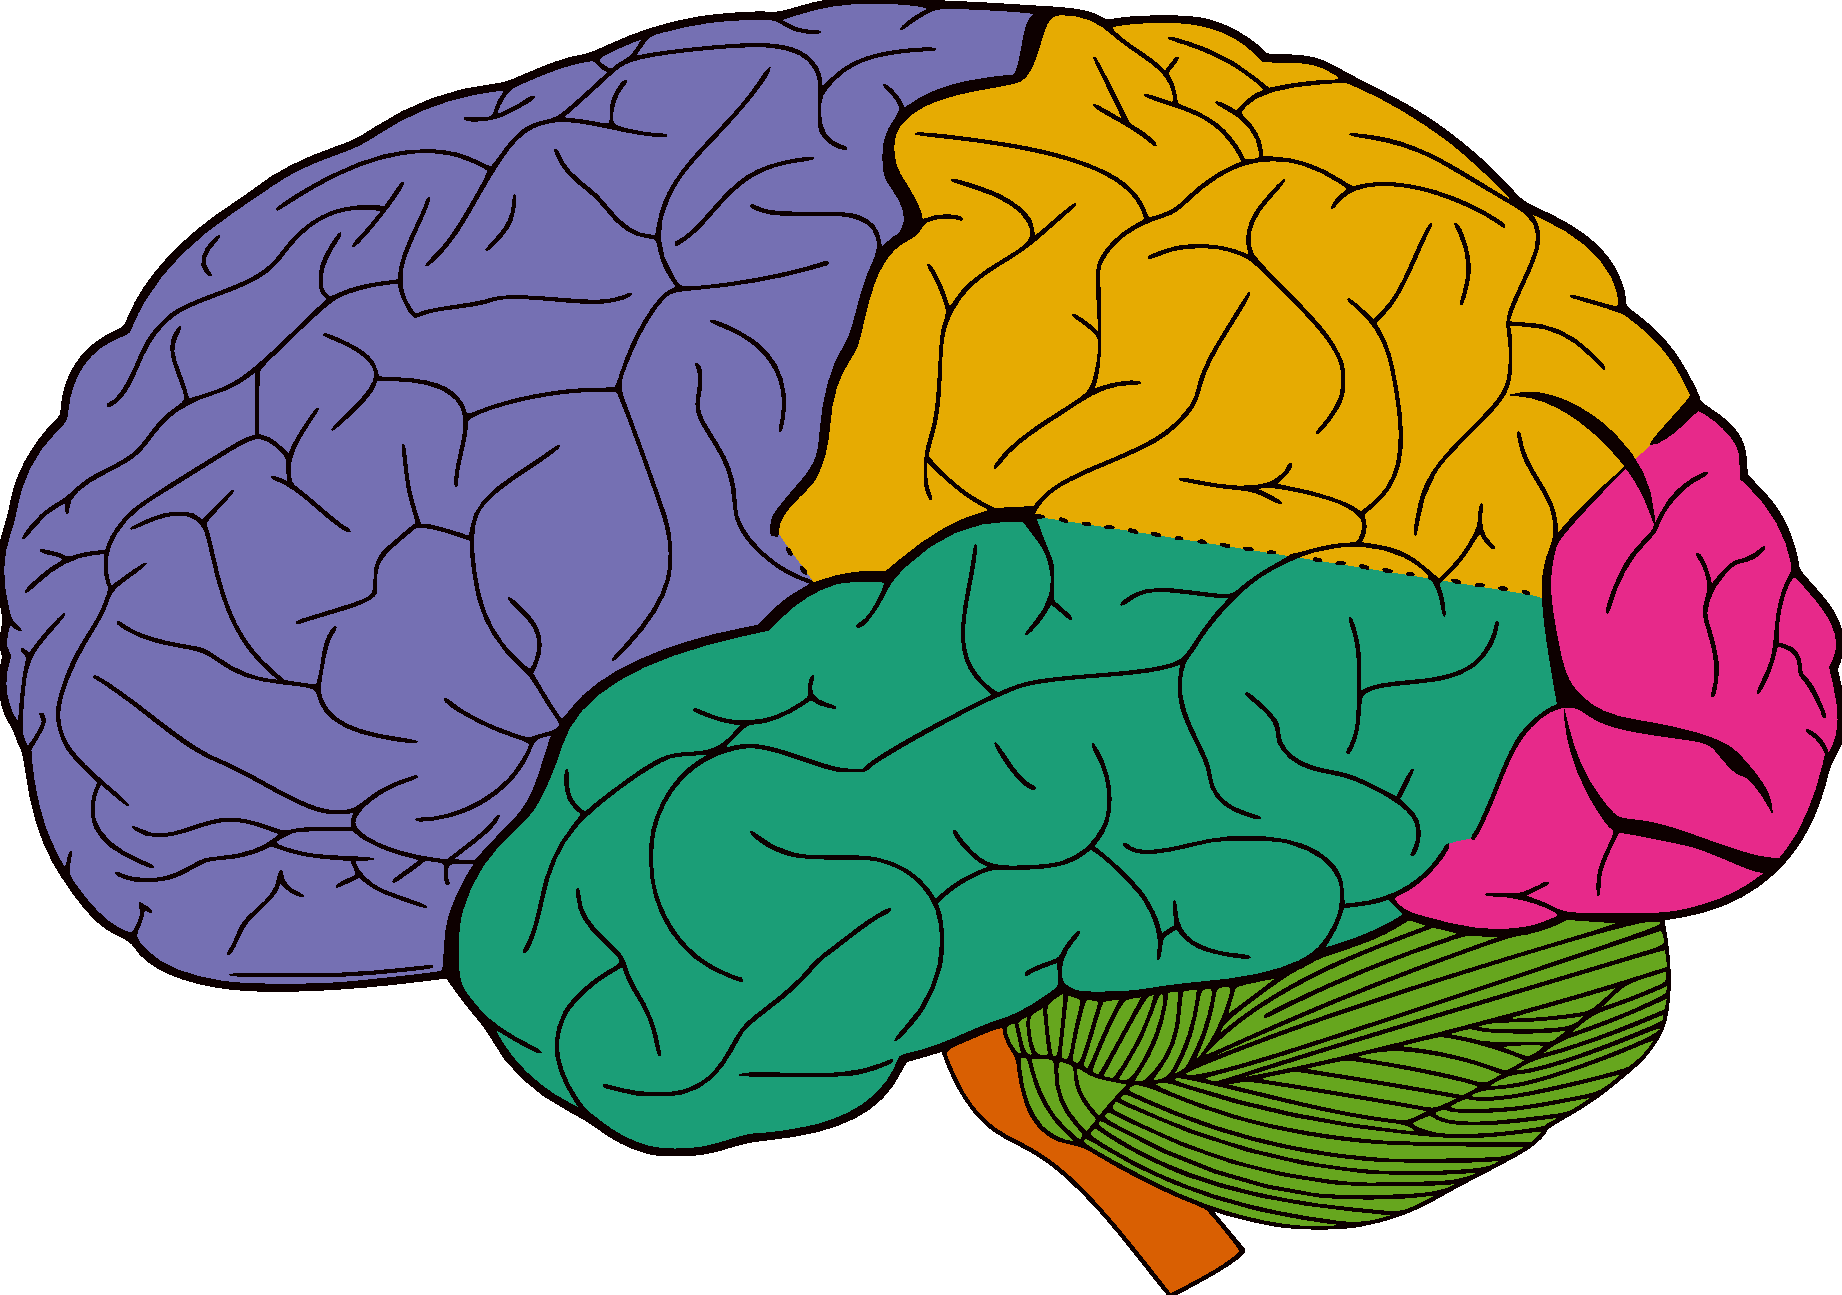
\includegraphics[height=0.3\textwidth]{gfx/neuroanatomy/brain_lobes.pdf}}
\hfill
\tikzset{external/export next=false}
\subcaptionbox{%
        \label{fig:coronalStained}%
        \todo{BB 4201} Coronal section stained for cell bodies. The \ac{GM} is dark while the \ac{WM} is bright. The left and right hemisphere is connected via the corpus calosum.}%
    [0.47\textwidth]{\includegraphics[height=0.3\textwidth]{dev/brain/BB_4201.png}}
    % \begin{tikzpicture}[]
    %     \node[inner sep=0pt, anchor = south west] (fig) at (0,0)
    %     {\includegraphics[height=0.3\textwidth]{dev/brain/BB_4201.png}};
    %     \coordinate (WM1) at ($(fig.north west)!0.6!(fig.north east)$);
    %     \coordinate (WM2) at ($(fig.north east)!0.35!(fig.south east)$);
    %     \draw[RED, ultra thick, <-] (WM1 |- WM2) -- ++ (-42:0.75) node[pos=1, anchor=north] {\textbf{WM}};
    %     \coordinate (GM1) at ($(fig.north west)!0.275!(fig.north east)$);
    %     \coordinate (GM2) at ($(fig.north east)!0.125!(fig.south east)$);
    %     \draw[GREEN, ultra thick, <-] (GM1 |- GM2) -- ++ (-65:0.75) node[pos=1, anchor=north] {\textbf{GM}};
    % \end{tikzpicture}
% }
\caption{Illustration of the human brain and a cell body stained coronal section.}
\label{fig:humanBrain}
\end{figure}
%
The cerebellum and cerebrum contain a \ac{GM} stucture at the brain surface.
This structure is filled with neurons.
These cells have the task of processing the information of all signals coming from inside and outside of the brain.
These cells are arranged in cortical layers that have different thicknesses, cell types, and densities specific to a brain area.
These cells have a relatively high density and are not only locally interconnected with each other, but connect also with different brain areas.
%  (see \cref{fig:nerveFiber,fig:cortLayers}).
Therefore, the folding of the brain is particularly important to increase the surface and therefore the number of cells.
In the human brain there are several billions of nerve cells.
There are many types of cells, \eg{} granule or pyramidal cells.
The highly interconnected structure and arrangement of the various cells is the source of its high number of different functionalities.
It is imporatant to investiagte the human brain to gain a better understanding of the brain's function and an improved understanding of pathophysiological processes that may lead to improved medical treatment of brain deseases.
%
%
%
\section{Fiber architecture} \label{sec:fiberArchitecture}
%
\begin{figure}[!t]
\centering
% \subcaptionbox{
%     \label{fig:cortLayers}
%     Cortical layers \todo{wichtig?}
%     }[0.225\textwidth]{\includegraphics[height=4.5cm]{dev/wiki/layers.png}}
% \hfill
\tikzset{external/export next=false}
% \subcaptionbox{
%     \label{fig:nerveCell}
%     Nerve cell structure.
% }[0.75\textwidth]{
\begin{tikzpicture}[every node/.style={font=\small,},]
    \node[inner sep=0pt, anchor = south west] (fig) at (0,0) {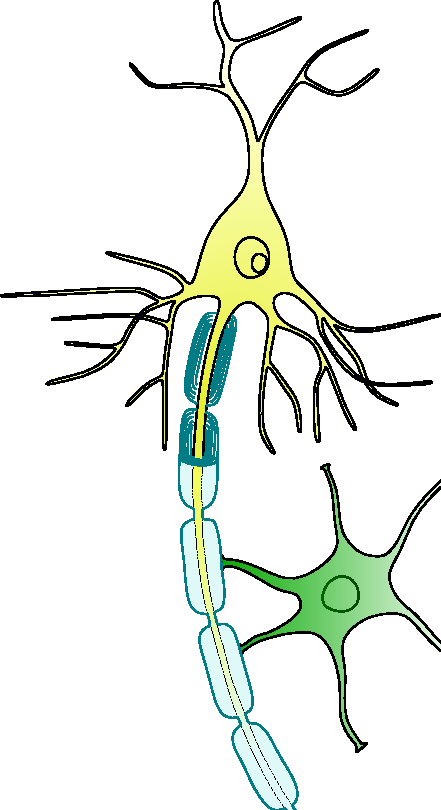
\includegraphics[ angle=90,width=0.75\textwidth]{gfx/neuroanatomy/neuron-axon.pdf}}; %height=4.2cm
    \begin{scope}[overlay]
        % \foreach \p in {0,0.1,0.2,0.3,0.4}{
        %     \draw[blue] (rel cs:name=fig,x=\p,y=\p) rectangle (rel cs:name=fig,x=1-\p,y=1-\p);
        % }
        % 
        \node[anchor=south] at (rel cs:name=fig,x=0.72,y=1.025) {Oligodendrocyte};
        \node[anchor=north] at (rel cs:name=fig,x=0.235,y=0.22) {Cell Body};
        \node[anchor=west] at (rel cs:name=fig,x=1,y=0.675) {Axon};
        \node[anchor=north] at (rel cs:name=fig,x=0.7,y=0.4) {Myelin};
        \draw[<-] (rel cs:name=fig,x=0.9,y=0.5) -- ++(-69:0.5) node[pos=1,anchor=north] {Node of Ranvier};
        \draw[<-] (rel cs:name=fig,x=0.295,y=0.53) -- ++(-140:0.75) node[pos=1,anchor=north] {Nucleus};
        \node[anchor=south] at (rel cs:name=fig,x=0.24,y=0.8) (D) {Dendrites};
        \draw[->] (rel cs:name={D},x=0.3,y=0) -- ++(-155:0.6){};
        \draw[->] (rel cs:name={D},x=0.7,y=0) -- ++(-25:0.6){};
    \end{scope}
    \path[] ($(fig.south west)-(0,0)$) rectangle ($(fig.north east)+(1,0.75)$);
\end{tikzpicture}
% }
\caption{Illustration of a neuron with axon and oligodendrocytes. The olegodendrocyte build up a layered lipid structure up, surrounding the axon. The myelin layers are separated along the axon by nodes of Ranvier.}
\label{fig:CortexAndNerveCell}
\end{figure}
%
Nerve cells are connected by nerve fibers.
A typical nerve cell (see \cref{fig:nerveCell}) comprises a cell body, called a soma, that processes incoming information.
The information arrives via dendrites, which are star-shaped branches.
The axon is the cell's only information output.
It travels through the brain often associated with nerve fiber bundles to its destination, where it connects with the axon terminal to other neurons.
\par
%
The axon is surrounded by a myelin sheath, a lipid layered structure deriving from nearby olegodendrides (see \cref{fig:human-brain}).
The myeling electrically insulates the axon and improves the speed of propagation of the electrical action potential along the axon and also its signal strength.
The diamater of the myelin ranges from about $\SI{0.5}{\micro\meter}$ to several $\si{\micro\meter}$ (see \cref{tag:axonDiameter}).
There are many different types of axons.
Some contain a very thick myelin layer, while others have none.
The high density of axons and myelin makes the brainappear white and is therefore called \ac{WM}, whereas the outer cell bodys appear darker and ist called \ac{GM}.
This color difference is clearly visible in a Nissle stained histological sections (see \cref{fig:coronalStained}).
\par
%
To enhance the contrast of the nerve fibers to the background, staining like Nissle is used to darken the myelin (see \cref{fig:brainMyelinStain}).
This allows to follow small nerve fibers down to individual nerves depending on their myelination degree.
Larger nerve fiber bundles are such dark, that mostly no orientation can be exracted.
\par
% 
\Cref{fig:brainMyelinStain} shows a nissle stained brain section.
% Both single nerve fibers and nerve fiber bundles are visible.
Between neurons, individual nerve fibers form complex reticular structures.
Several nerve fiber bundles trace their paths through the thalamus and are visible as dark structures.
% 
A closer look with an electron microscope into a nerve fiber bundle of the corpus callosum of a rodent is shown in \cref{fig:elecMic}.
The nerve fibers of the $\SI{100}{\nano\meter}$ thin section are densely packed together.
Axon diameter and myelin thickness vary from nerve fiber to nerve fiber.
% 
\begin{figure}[!t]
	\centering
    \tikzset{external/export=false}
    \subcaptionbox{%
        \label{fig:brainMyelinStain}
        Myelin staining of the human thalamus, sagital section. \textcolor{Orange}{Nerve fiber bundle} structures are visiable as as cut structures visible as elliptical dark shape. In between \textcolor{ProcessBlue}{net-like structures} are fromed from individual nerve fibers. \url{http://brainmaps.org/HBP3/h.sapiens/sag/h5thal-myelin/17a}}
    [.49\textwidth]{
        \begin{tikzpicture}[]  
            \node[inner sep=0pt, anchor = south west] (fig) at (0,0)
            {\includegraphics[width=0.49\textwidth, trim=281 152 0 0, clip]{gfx/neuroanatomy/NeuralNet-BrainAtlasDotOrg.png}};
            %  
            \draw[Orange, ultra thick] (rel cs:name=fig,x=0.42,y=0.49) ellipse (0.75 and 0.375);
            \draw[ProcessBlue, ultra thick] (rel cs:name=fig,x=0.7,y=0.3) ellipse (1.1 and 0.7);
            % 
            \draw[white, ultra thick] let
                \p1=(rel cs:name=fig,x=0,y=0), 
                \p2=(rel cs:name=fig,x=0.1041,y=0), 
                \n1={veclen(\x1-\x2,\y1-\y2)}
            in
                ($(fig.south east)+(-0.2,0.2)$) -- ++ (180:\n1) node[above, midway, anchor=south]{$\SI{50}{\micro\meter}$};
        \end{tikzpicture}        
    }
    \hfill
    \subcaptionbox{%
        \label{fig:elecMic} Electron microscope image of a $\SI{100}{\nano\meter}$ thin section of rodent corpus callosum \cite{WALHOVD20142}. The myelin is visible as dark soroundings around the inner axon.}
    [.49\textwidth]{
        \begin{tikzpicture}[]  
            \node[inner sep=0pt, anchor = south west] (fig) at (0,0)
            {\includegraphics[width=0.49\textwidth]{dev/brain/elec_micrograph_rodent_cc.jpg}};
            \draw[white, ultra thick] let
                \p1=(rel cs:name=fig,x=0,y=0), 
                \p2=(rel cs:name=fig,x=0.1347,y=0), 
                \n1={veclen(\x1-\x2,\y1-\y2)}
            in
                ($(fig.south east)+(-0.2,0.2)$) -- ++ (180:\n1) node[above, midway, anchor=south]{$\SI{1}{\micro\meter}$};
        \end{tikzpicture}
    }
\end{figure}
% 
%
%
\section{Axon Literature}
\label{sec:axonMicroscopy}
%
\Cref{tab:axonDiameter} lists the results of the nerve fiber diameter.
The diameter and their standard deviation are region-specific.
The $g_{\mathit{ratio}}$ describes the fraction of the axon to the entire nerve fiber diameter.
From studies with \ac{dMRI} and electron microscopy
\cite{Stikov2015,Dean2016,Mohammadi2015,Cercignani2017,Berman2018,Jung2018} the $g_{\mathit{ratio}}$ is in the range of $\SI{0.6}{}$ to $\SI{0.9}{}$, depending on the region (see \cref{tab:gratio}).
%
\begin{table}[!b]
\centering
\pgfplotstabletypeset[
    thesisTableStyle,
    font=\footnotesize,
    % col sep=comma,
    columns/area/.style={string type},
    columns/mean/.style={string type},
    columns/std/.style={string type},
]{
    area mean std
    {sup. longitudinal fascide} $\SI{0.8}{\micro\meter}$ $\SI{0.2}{\micro\meter}$
    {Unicate/inferior occipital fasc.} $\SI{0.51}{\micro\meter}$ $\SI{0.05}{\micro\meter}$
    {corpus calosum} $\SI{0.69}{\micro\meter}$ $\SI{0.04}{\micro\meter}$
}
\caption{Nerve fiber diameter distribution of the human brain. Mean values over three human brains \cite{Liewald2014}.}
\label{tab:axonDiameter}
\end{table}
%
\begin{table}[!b]
\centering
\pgfplotstabletypeset[
thesisTableStyle,
font=\footnotesize,
col sep=semicolon,
columns={article,cite,gratio},
columns/article/.style={string type, column name=study, column type = {l}},
columns/cite/.style={string type, column name=cite, column type = {l}},
columns/gratio/.style={string type, column name=$g_{\mathit{ratio}}$},
]{data/gratio.csv}
\caption{human $g_{\mathit{ratio}}$ from invivo mri studies.}
\label{tab:gratio}
\end{table}
%
\cleardoublepage
\setcounter{chapter}{2}
\chapter{Theory}
\label{sec:theory}
% 
\cleanchapterquote{The first principle is that you must not fool yourself and you are the easiest person to fool.}{Richard P. Feynman}{}%\newline
%
\section{Introduction}
The following section lists the physical theories needed to describe the mathematics behind \ac{3D-PLI}. This includes the basic properties of light with the description of their polarization state, the optical models of the tissue, i.e. the nerve fibers and the mathematical description of the experimental setup of \ac{3D-PLI} and the analysis of its signal. The first part of this chapter was written with the help of \cite{demtroeder2, Fliebach2012}.
% 
% 
% 
\section{Electromagnetic Wave}
% 
Light is an electromagnetic wave. Electromagnetism is first fully described by James Clerk Maxwell. He formulated the Maxwell-Equations \cref{eq::maxwell_general}, generalized from the previous work of Johann Carl Friedrich Gau{\ss}, Michael Faraday and Andr\'{e}-Marie Amp\`{e}re and others:
% 
% \begin{align} 
% \begin{split} \label{eq::maxwell_macro}
%     \nabla \cdot \vec{D} &= 4\pi\rho_\text{f}\\
%     \nabla \cdot \vec{B} &= 0\\
%     \nabla \times \vec{E} &= -\frac{1}{c} \frac{\partial \vec{B}} {\partial t}\\
%     \nabla \times \vec{H} &= \frac{1}{c} \left(4\pi\vec{J}_\text{f} + \frac{\partial \vec{D}} {\partial t} \right)
% \end{split}
% \end{align}
% 
\begin{align} 
\begin{split} \label{eq::maxwell_general}
    \nabla \cdot \vec{E} &= \frac {\rho} {\varepsilon_0}\\
    \nabla \cdot \vec{B} &= 0\\
    \nabla \times \vec{E} &= -\frac{\partial \vec{B}} {\partial t}\\
    \nabla \times \vec{B} &= \mu_0\left(\vec{j} + \varepsilon_0 \frac{\partial \vec{E}} {\partial t} \right)
\end{split}
\end{align}
% 
with $\nabla \coloneqq \left({\frac{\partial}{\partial x}}, {\frac{\partial}{\partial y}}, {\frac{\partial}{\partial z}} \right)$ as vector differential operator, $\vec{E}$ as eletric field, $\rho$ as electric charge density, $\varepsilon_0$ as permittivity of free space, $\vec{B}$ as magnetic field, $\mu_0$ as permeability of free space and $\vec{j}$ as electric current density.
% 
The first equation states no electric field can be generated without an electric charge (charge conservation).
The second equation states, magnetic monopoles does not exists. The basic entity of an magnetic field is a dipole.
The third and forth equation show the interconnection of the electric and magnetic fields in space and time.
A change in the electric field yields to a magnetic field and vice versa.
Equation forth additional indicates the creation of a magnetic field from a electric current $\vec{j}$.
The maxwell equation fullfill the continoiut ... $\divergence j + \frac{\partial \rho}{\partial t} = 0$.
This means that neither an electric of magnetc field can be created without either an electric current or a change of electric potential.
%
% \par
% 
\subsection{EM in a vacuum}
% 
In a vacuum this simplifies with $\rho = 0$ and $\vec{j} = \vec{0}$ to:
% 
\begin{align}
\begin{split} \label{eq::maxwell_vacuum}
  \nabla \cdot \vec{E} &= 0 \quad\\
  \nabla \cdot \vec{B} &= 0 \quad\\
  \nabla \times \vec{E} &= -\frac{\partial\vec B}{\partial t}\\
  \nabla \times \vec{B} &= \mu_0\varepsilon_0 \frac{\partial\vec E}{\partial t}
  \end{split}
\end{align}
% 
With 
\begin{align}
\begin{split} 
    \nabla \times \nabla \times \vec{E} = -\nabla \times \frac{\partial \vec{B}} {\partial t} &= -\frac{\partial} {\partial t} \left( \nabla \times  \vec{B} \right)\\
    &= -\varepsilon_0 \cdot \mu_0 \frac{\partial^2 \vec{E}}{\partial t^2} \, ,
\end{split}
\end{align}
% 
the identity $\nabla \times \left( \nabla \times \vec{A} \right) = \nabla(\nabla \cdot \vec{A}) - \nabla^{2}\vec{A}$ and $\mu_0\varepsilon_0 = \frac{1}{c^2}$, with $c$ as the speed of light\footnote{can be derived from Maxwells equation and Lorentz force in a vacuum}, this further simplifies to:
% 
\begin{align}
\begin{split} \label[pluralequation]{eq::maxwell_wave_equations}
  \frac{1}{c^2} \frac{\partial^2 \vec{E}}{\partial t^2} - \nabla^2 \vec{E} &= 0 \\
  \frac{1}{c^2} \frac{\partial^2 \vec{B}}{\partial t^2} - \nabla^2 \vec{B} &= 0
\end{split}
\end{align}
% 
% Another common representation is
% % 
% \begin{align}
% \begin{split} \label{eq::maxwell_wave_equations_box}
%   \Box \ \vec{E} &= 0 \\
%   \Box \ \vec{B} &= 0
% \end{split}
% \end{align}
% 
% with the help of the d'Alembert operator $\Box \coloneqq \partial^a\partial_a = \nabla^2 - \frac{1}{c^2} \frac{\partial^2}{\partial t^2}$.
% 
This also shows that $c^2  \frac{\partial B} {\partial z} = \frac{\partial E}{\partial t} \Rightarrow \vec{E} \cdot \vec{B} = 0$ and therefore the electric and magnetic field components are perpendicular to each other.
Additionally it also means, that space and time are interconnected and that light travels in vacuum with the speed of light $c$.
% 
\subsection{Solving MW Equ in vacuum}
% 
\Cref{eq::maxwell_wave_equations} have the shape of a wave equation and can therefore as known be solved by
% 
% Using the Maxwell equation in vacuum \ref{eq::maxwell_vacuum}, one can find the most simple solution to the differential equation is a wave:
% 
\begin{align}
\begin{split} \label{eq::dgl_solution}
  \vec{E}( \vec{r}, t ) &= g(\phi( \vec{r}, t )) = g( \omega t - \vec{k} \cdot \vec{r} + \varphi)\\
  \vec{B}( \vec{r}, t ) &= g(\phi( \vec{r}, t )) = g( \omega t - \vec{k} \cdot \vec{r} + \varphi )
\end{split}
\end{align}
% 
where $g$ is any well behaved function (continuous and differentiable) and therefore also their superposition.
% 
With the help of
% 
\begin{align}
k = \mathopen| \vec{k} \mathclose| = \frac{\omega}{c} =  \frac{2 \pi}{\lambda}
\end{align}
% 
a planar wave can be descriped by
% 
\begin{align}
\begin{split} \label{eq::plane_wave}
\vec{E}(\vec{r}) &= \vec{E}_0 \cdot e^{ -i \, \vec{k} \cdot \vec{r} }\\
 \vec{B}(\vec{r}) &= \vec{B}_0 \cdot e^{ -i \, \vec{k} \cdot \vec{r} }
\end{split}
\end{align}
% 
with $\vec{k}$ as Wave vector pointing into the travel direction of the light wave.
% 
% 
\subsection{Polarization}
% 
\begin{figure}[!t]
\centering
\setlength{\tikzwidth}{\textwidth}
\inputtikz{gfx/pli/polarization_state}
\label{fig:polarization_state}
\caption{Illustration of light polarization state. Unpolarized light goes throug a linear polarizer which polarizes the light in one direction (w.l.o.g. $E_x$ and $E_y$ in phase). Afterwords it travels though a quarter wave retarder, which turn linear polarized light (of a specific wave length) into circular polarized light, where w.l.o.g. $E_x$ and $E_y$ are $\pi/2$ phase}
\end{figure}
% 
Since the light wave travels into one direction, and the electric field and magnetic field are perpendicular to $\vec{k}$ as well to each other, there orientation is a fundamental property of light called polarization.
Without any additional info, the polarization orientation is conventional in the direction of the electric field component.
% 
A superposition of x and y wave with z equal to direction of propagation yield w.l.o.g. to the general form
\begin{align}
\vec{E}(z,t) &= \begin{pmatrix} E_{0x} \cdot e^{ -i \phi_x } \\ E_{0y} \cdot e^{ -i \phi_y } \\ 0 \end{pmatrix}
e^{ -i (kz - \omega t)}
\end{align}
%
\begin{figure}[!t]
\centering
\tikzset{external/export=false}
%
% \captionsetup[sub]{textfont=normalsize}
% \captionsetup[sub]{position=top, skip=-14pt}
\tikzset{cross/.pic={
\draw[arrows={-Latex[scale=1]}] (-{sqrt(2)},0) -- ({sqrt(2)},0) node[anchor=north]{\small $E_x$};
\draw[arrows={-Latex[scale=1]}] (0,-{sqrt(2)}) -- (0,{sqrt(2)}) node[anchor=east]{\small $E_y$};
}}
%
% \subcaptionbox{}[.3\textwidth]{
\begin{tikzpicture}
\begin{scope}[shift={(0,0)}, local bounding box=A]
\pic at (0,0) {cross};
% \draw[] (0, 2) node[font=\small] () {linear, horizontal};
\draw[very thick, arrows={Latex[scale=1]-Latex[scale=1]}] (-1, 0) -- (1, 0);
\draw[] (0, -2) node () {$\begin{pmatrix} 1&0 \end{pmatrix}$};
\draw[] (0, -2.75) node () {$\begin{pmatrix} 1&1&0&0 \end{pmatrix}$};
\end{scope}
\node[anchor=south west, xshift=-1em] at (A.north west) {\small \textcolor{magenta}{\textbf{(a)}} linear, horizontal};
% }\hfill
% \subcaptionbox{}[.3\textwidth]{
\begin{scope}[shift={(4,0)}, local bounding box=B]
\pic at (0,0) {cross};
% \draw[] (0, 2) node[font=\small] () {linear, vertical};
\draw[very thick, arrows={Latex[scale=1]-Latex[scale=1]}] (0, -1) -- (0, 1);
\draw[] (0, -2) node () {$\begin{pmatrix} 0&1 \end{pmatrix}$};
\draw[] (0, -2.75) node () {$\begin{pmatrix} 1&-1&0&0 \end{pmatrix}$};
\end{scope}
\node[anchor=south west, xshift=-1em] at (B.north west) {\small \textcolor{magenta}{\textbf{(b)}} linear, vertical};
% }\hfill
% \subcaptionbox{}[.3\textwidth]{
\begin{scope}[shift={(8,0)}, local bounding box=C]
\pic at (0,0) {cross};
% \draw[] (0, 2) node[font=\small] () {linear, $\pi/4$};
\draw[very thick, arrows={Latex[scale=1]-Latex[scale=1]}] (-1, -1) -- (1, 1);
\draw[] (0, -2) node () {$\begin{pmatrix} 1&1 \end{pmatrix}$};
\draw[] (0, -2.75) node () {$\begin{pmatrix} 1&0&1&0 \end{pmatrix}$};
\begin{scope}[overlay]
\draw[] (2, -2) node () {Jones};
\draw[] (2, -2.75) node () {Stokes};
\end{scope}
\end{scope}
\node[anchor=south west, xshift=-1em] at (C.north west) {\small \textcolor{magenta}{\textbf{(c)}} linear, $\pi/4$};
% }
% \\[2em]
% \subcaptionbox{}[.32\textwidth]{
\begin{scope}[shift={(0,-5.75)}, local bounding box=D]
\pic at (0,0) {cross};
% \draw[] (0, 2) node[font=\small] () {left circular};
\draw[very thick] plot[domain=0:360,samples=90,smooth] ({cos(\x)},{sin(\x)});
\draw[very thick, arrows={-Latex[scale=1]}] plot[domain=44:45,samples=1] ({cos(\x)},{sin(\x)});
\draw[very thick, arrows={-Latex[scale=1]}] plot[domain=224:225,samples=1] ({cos(\x)},{sin(\x)});
\draw[] (0, -2) node () {$\begin{pmatrix} 1&i \end{pmatrix}$};
\draw[] (0, -2.75) node () {$\begin{pmatrix} 1&0&0&-1 \end{pmatrix}$};
\end{scope}
\node[anchor=south west, xshift=-1em] at (D.north west) {\small \textcolor{magenta}{\textbf{(d)}} left circular};
% }\hfill
% \subcaptionbox{}[.32\textwidth]{
\begin{scope}[shift={(4,-5.75)}, local bounding box=E]
\pic at (0,0) {cross};
% \draw[] (0, 2) node[font=\small] () {right circular};
\draw[very thick] plot[domain=0:360,samples=90,smooth] ({cos(\x)},{sin(\x)});
\draw[very thick, arrows={-Latex[scale=1]}] plot[domain=46:45,samples=1] ({cos(\x)},{sin(\x)});
\draw[very thick, arrows={-Latex[scale=1]}] plot[domain=226:225,samples=1] ({cos(\x)},{sin(\x)});
\draw[] (0, -2) node () {$\begin{pmatrix} 1&-i \end{pmatrix}$};
\draw[] (0, -2.75) node () {$\begin{pmatrix} 1&0&0&1 \end{pmatrix}$};
\end{scope}
\node[anchor=south west, xshift=-1em] at (E.north west) {\small \textcolor{magenta}{\textbf{(e)}} right circular};
% }\hfill
% \subcaptionbox{}[.32\textwidth]{
\begin{scope}[shift={(8,-5.75)}, local bounding box=F]
\pic at (0,0) {cross};
% \draw[] (0, 2) node[font=\small] () {unpolarized};
\draw[] (0, -2.75) node () {$\begin{pmatrix} 1&0&0&0 \end{pmatrix}$};
\begin{scope}[overlay]
\draw[] (2, -2) node () {Jones};
\draw[] (2, -2.75) node () {Stokes};
\end{scope}
\end{scope}
\node[anchor=south west, xshift=-1em] at (F.north west) {\small \textcolor{magenta}{\textbf{(f)}} unpolarized};
%
\path[] ($(A.west)!-0.075!(C.east)$) -- ($(A.west)!1.075!(C.east)$);
\end{tikzpicture}
% }
%
\caption{polarization states, check vector length,\itodo{test speed}} 
\label{fig:polarization_state_vectors}
\end{figure}
%
\Cref{fig:polarization_state_vectors} shows another representation of the polarization sate of a light wave.
It show the component perpendicular to the travelling direction.
Therefore the time variation can be shown on the xy-plane.
Additionally the states can be describe by the Jones or Stokes calculus, later described in \cref{sec:jones,sec:mueller_stokes}.
% 
% 
% 
\subsection{Light in medium}
% 
The Maxwell equations in \dummy{} are described above. They can be solved analog to \dummy{}. This yields to some special behavior, \eg{} the magnetic and electric field component get out of phase.
However here only the two properties of absorption and diffraction are described.
They derivation can be found \eg{} \cite{demtroeder2, Fliebach2012}.
% 
\subsection{Absorption}
% 
\begin{align}
    I = I_0 \exp(-\mu x)
\end{align}
\todo{herleiten}
% 
Beersche law of absorption with $\mu = \frac{4\pi \kappa}{\lambda_0}$ where $\kappa$ is the imaginary part of the complex refractive index.
% 
\subsection{Refraction}
% 
\begin{figure}[!t]
\centering
\setlength{\tikzwidth}{\textwidth}
\inputtikz{gfx/pli/refraction}
\label{fig:optic_refraction}
\caption{Illustration of refraction.}
\end{figure}
% 
Refraction is the property of light to change direction as it passes from one medium to another. This can be shown by using the full Maxwell equations  for non-conductive material, \ie{} $\vec{j} = 0, \rho = 0$, that the differential equating consist out of a primary wave with from atomic medium induced secondary waves, which leads to a reduction of the velocity of the resulting wave. Mathematically this can be described by a complex number $n = c' / c$.
Using this relationship at a boundary surface between two media, one can show that the incident light beam splits into a reflecting and transmitting light wave. The reflecting light wave has the same angle as the incident light beam relative the the surface normal. The transmitting light beam however due to the reduction of the velocity, changes its direction described by the Snellius law
\begin{align}
    n_0 \sin \alpha = n_1 \sin \beta
\end{align}

% 
\begin{align}
\underline{n} = n + i\kappa
\end{align}
% 
\begin{align}
\begin{split}
\vec{E}(z, t) &= \operatorname{Re}\! \left[\vec{E}_0 \cdot e^{i\, (kz - \omega t)}\right] \\
&= \operatorname{Re}\! \left[\vec{E}_0 \cdot e^{i\, (2\pi(n + i\kappa)z/\lambda_0 - \omega t)}\right] \\
&= e^{-2\pi \kappa z/\lambda_0} \operatorname{Re}\! \left[\vec{E}_0 \cdot e^{i\, (kz - \omega t)}\right]
\end{split}
\end{align}\todo{?}
% 
% 
% 
\subsection{Birefingence}
%
\begin{figure}[!t]
\centering
\setlength{\tikzwidth}{\textwidth}
\inputtikz{gfx/pli/retardation}
\caption{Illustration of retardation.}
\label{fig:optic_retardation}
\end{figure}
% 
\begin{figure}[!t]
\centering
\subcaptionbox{}[.49\textwidth]{
\setlength{\tikzwidth}{0.49\textwidth}
\inputtikz{gfx/pli/ellipsoid_a}}
\subcaptionbox{}[.49\textwidth]{
\setlength{\tikzwidth}{0.49\textwidth}
\inputtikz{gfx/pli/ellipsoid_b}}
\caption{birefringence elipsoid}
\label{fig:index_elipsoid}
\end{figure}
% 
Material can have a different refractive index depending on the relative orientation and polarization of the light beam.
This property is known as birefringence.
The refractive index can be described as the refractive index $n_o$ and extraordinary  $n_e$.
Since these two are perpendicular to each other, one can split the light beam into the same perpendicular parts and describe each by its own.
These two light beams, except for the trivial case of a light beam is perpendicular to the surfave, have a different direction.
However for small relative length (hängt von n ab, bzw der phasenänderung) the two light beams leave the material at the same point and recombined at the end.
The change of phase is called birefringence and is described by the difference between the .. and ...
% 
\begin{align}
    \Delta n = n_e - n_o \> .
\end{align}
% 
This .. can be visualized by the index ellipsoid \cref{fig:index_elipsoid}.
The change of the amplitude and phase can be described by the following two vector matrices descriptions.
% 
% 
% 
\subsection{Jones calculus}
\label{sec:jones}
% 
The Jones calculus, introduced by Robert Clark Jones in 1941, describes the polarization state of a light beam by a complex vector $J$:
% 
\begin{align}
    \vec{J} = \begin{pmatrix} E_x \exp(i \phi_x) \\ E_y \exp(i \phi_y) \end{pmatrix}
\end{align}
% 
The amplitude of the perpendicular components are $E_x$ and $E_y$ with their phase $\phi_x$ and $\phi_y$.
Optical elements, which changes the polarization state, such as a polarization filter and retarder, can be desribed by a matrix:
% 
\begin{align}
\begin{split}
\mat{P}_x = 
\begin{pmatrix}
1 & 0 \\ 0 & 0
\end{pmatrix}
, \,
\mat{P}_y = 
\begin{pmatrix}
0 & 0 \\ 0 & 1
\end{pmatrix}
, \,
\mat{M} =
\begin{pmatrix}
e^{i \varphi_x} & 0 \\ 0 & e^{i \varphi_y}
\end{pmatrix}
, \,
\Lambda_{1/4}=
e^{\frac{i \pi}{4}}
\begin{pmatrix}
1 & 0 \\ 0 & -i
\end{pmatrix}
\end{split}
\end{align}
% 
A rotation of an optical element can be achieved by a 2d rotation matrix $\mat{R}$:
% 
\begin{align}
\begin{split}
\mat{M}(\theta )=\mat{R}(\theta )\cdot\mat{M}\cdot\mat{R}(-\theta )
, \>
\mat{R}(\theta ) = 
\begin{pmatrix}
\cos \theta & -\sin \theta \\
\sin \theta & \cos \theta
\end{pmatrix}
\end{split}
\end{align}
% 
% 
% 
\subsection{M\"uller-Stokes}\label{sec:Mueller-Stokes}
\label{sec:mueller_stokes}
% 
Analog to \cref{sec:jones} the M\"uller-Stokes formalism, described by George Gabriel Stokes in 1852, also describes the polarization state (how good is it \dummy{}) of a light beam.
However it does not use the absolute .. but the relative polarization between both components:
% 
\paragraph{Stokes vector}
\begin{align}
\begin{split}
S_0 &= I \\
S_1 &= I p \cos 2\psi \cos 2\chi \\
S_2 &= I p \sin 2\psi \cos 2\chi \\
S_3 &= I p \sin 2\chi
\end{split} \hspace{-6em}
\begin{split}
& \equiv \langle E_x^{2} \rangle + \langle E_y^{2} \rangle \\
%  & = \langle E_a^{2} \rangle + \langle E_b^{2} \rangle \\
%  & =  \langle E_l^{2} \rangle + \langle E_r^{2} \rangle \\
& \equiv \langle E_x^{2} \rangle - \langle E_y^{2} \rangle \\
& \equiv \langle E_a^{2} \rangle - \langle E_b^{2} \rangle \\
& \equiv  \langle E_l^{2} \rangle - \langle E_r^{2} \rangle
\end{split}
, \,
\vec{S} =
\begin{pmatrix} S_0 \\ S_1 \\ S_2 \\ S_3\end{pmatrix}
\end{align}
% 
% \begin{align}
% \begin{split}
% S_0 & \equiv \langle E_x^{2} \rangle + \langle E_y^{2} \rangle \\
%  & = \langle E_a^{2} \rangle + \langle E_b^{2} \rangle \\
%  & =  \langle E_l^{2} \rangle + \langle E_r^{2} \rangle \\
% S_1 & \equiv \langle E_x^{2} \rangle - \langle E_y^{2} \rangle \\
% S_2 & \equiv \langle E_a^{2} \rangle - \langle E_b^{2} \rangle \\
% S_3 & \equiv  \langle E_l^{2} \rangle - \langle E_r^{2} \rangle
% \end{split}
% \end{align}
% 
Therefore the phase can not be described anymore.
However the relative phase information is stored and can be used to describe also polarization states of polarization filters, which can not be described by Jones.
Aanlog to Jones one can formulate the matrices for the optical components:
% 
\paragraph{Linear Polarizer}
\begin{align}
\mat{P}_x=\frac{1}{2}
\begin{pmatrix}
    1 & 1 & 0 & 0 \\
    1 & 1 & 0 & 0 \\
    0 & 0 & 0 & 0 \\
    0 & 0 & 0 & 0
  \end{pmatrix}
, \,
\mat{P}_y=\frac{1}{2}
\begin{pmatrix}
     1 & -1 & 0 & 0 \\
    -1 &  1 & 0 & 0 \\
     0 &  0 & 0 & 0 \\
     0 &  0 & 0 & 0
\end{pmatrix}
\end{align}
% 
\paragraph{retarder}
\begin{align}
\mat{M}=\
\begin{pmatrix}
    1 & 0 & 0 &  0 \\
    0 & 1 & 0 &  0 \\
    0 & 0 & \cos \delta & \sin \delta \\
    0 & 0 & -\sin \delta &  \cos \delta
\end{pmatrix}
\end{align}
% 
\paragraph{Quarter-wave plate (fast-axis vertical)}
\begin{align}
\Lambda_{1/4}=\
\begin{pmatrix}
    1 & 0 & 0 &  0 \\
    0 & 1 & 0 &  0 \\
    0 & 0 & 0 & -1 \\
    0 & 0 & 1 &  0
\end{pmatrix}
\end{align}
% 
\paragraph{Rotation Matrix}
\begin{align}
\mat{R}(\theta)=
\begin{split}
\begin{pmatrix}
    1 &                0 &               0 & 0 \\
    0 & \cos{(2\theta)} & -\sin{(2\theta)} & 0 \\
    0 & \sin{(2\theta)} & \cos{(2\theta)} & 0 \\
    0 &                0 &               0 & 1
  \end{pmatrix}
\end{split}
\end{align}
% 
Analog to \dummy{} rotations are applied by
\begin{align}
\mat{M}(\theta )=\mat{R}(\theta )\cdot\mat{M}\cdot\mat{R}(-\theta )
\end{align}
% 
% \section{Tissue Discretization}
% % 
% By deviding the volume into small diskreticed subvolumes, one can multiply the .. all together and ... (analog Riemann sum)
% \begin{align}
%     \int F \, dt \approx \sum_n F \, \Delta t
% \end{align}
% see simulation?
% 
%  see simulation
% \paragraph{Micro vs Macro:}
% % 
% % \begin{align}
% %   \int_{y_\textit{min}}^{y_\textit{max}} \vec{v}(y) \,dy\\
% %   x = const
% %   y = y(\alpha,x) = tan(\alpha) \cdot x\\
% %   \vec{v}_r = \begin{pmatrix} \cos(\alpha)\\ \sin(\alpha)\\0\end{pmatrix}, \, \vec{v}_p = \begin{pmatrix} 0\\ 0\\1\end{pmatrix}\\
% %   \vec{v}_r = \begin{pmatrix} \cos(\arctan(y/x))\\ \sin(\arctan(y/x))\\0\end{pmatrix}\\
% %   \int_{y_\textit{min}}^{y_\textit{max}} \vec{v}_p(y) \,dy = (y_\textit{max} - y_\textit{min}) \cdot e_z\\
% %   \int_{y_\textit{min}}^{y_\textit{max}} \vec{v}_r(y) \,dy = \int_{y_\textit{min}}^{y_\textit{max}} \cos(\arctan(y/x)) dy \cdot e_x \\
% %   = x\left(\sinh^{-1}(y_\textit{max}/x) - \sinh^{-1}(y_\textit{min}/x)\right) \\
% %   = 2x \left(\sinh^{-1}\left(\frac{2\sqrt{R-x^2}}{x}\right)\right)
% % \end{align}
% % 
% % \begin{align}
% %     % \frac{\oint \vec{v}_z \mathrm{d}A}{\oint \vec{v}_x \mathrm{d}A} = 
% %     % \frac{\int_{-1}^{1}\abs{\vec{v}} \mathrm{d}x}{\int_{-\frac{\pi}{2}}^{\frac{\pi}{2}} \abs{\vec{v}} \cos(\varphi) \mathrm{d}\varphi} =
% %     % \frac{2}{1}
% %     \frac{A_{\Box}}{A_{\circ}} = \frac{4}{\pi}
% % \end{align}
% % 
% \todo{why 2*dn?}
% 
\section{Experimental Setup}\label{sec:expSetup}
%
\begin{figure}[!t]
    \captionsetup[sub]{position=top}
    \setlength{\tikzwidth}{\textwidth}
	\centering
% 	\subcaptionbox{\label{setup-lap} \ac{LAP}}[\textwidth]{
% % 		\resizebox{0.95\textwidth}{!}{
% 		\inputtikz{gfx/pli/pli_setup}
% % 	}
% 	}\\
% 	\subcaptionbox{\label{setup-pm} \ac{PM}}[\textwidth]{
% % 		\resizebox{0.95\textwidth}{!}{
		\inputtikz{gfx/pli/pli_setup_pm}
% % 	}
% 	}
	\caption{Illustration of PLI setup.}
	\label{fig:pli_setup}
\end{figure}
%
% \begin{figure}[!t]
%     % \captionsetup[sub]{position=top}
%     \setlength{\tikzwidth}{0.3\textwidth}
% 	\centering
% 	\subcaptionbox{\ac{LAP}}[.45\textwidth]{\hfill
% 			\inputtikz{gfx/pli/pli_detail}\hfill}\hfill
% 	\subcaptionbox{\ac{PM}}[.45\textwidth]{\hfill
% 			\inputtikz{gfx/pli/pli_detail_pm}\hfill}
% 	\caption{Illustration of \acs{3D-PLI} setup.}
% 	\label{fig:pli_detail}
% \end{figure}
%
The \ac{3D-PLI} setup is described in \cite{Axer2011} with the tiltable light beam microscope (LMP) in \cite{Wiese:887678}.
For the routine measurements two (three) microscope systems are currently in use.
The first use of a high throughput microscope is the \ac{LAP} with a pixel size of about \SI{60}{\micro\meter}.\footnote{can be change by the optic also to $\SI{40}{\micro\meter}$ and $\SI{20}{\micro\meter}$, but remains for the routine measurements with $\SI{60}{\micro\meter}$.}
It consist out of a led light source (\SI{525}{\nano\meter}), a rotatable polarization filter, a rotatable quarter wave retarder, the specimen stage, which can be tilted for oblique views, a rotatable polarizer.
Both polarizer and quarter wave retarder are rotated at the same time.
The both polarizers have a phase offset of $\SI{90}{\degree}$, the first polarizer and the quarter wave retarder of $\SI{45}{\degree}$ (see (see \cref{setup-lap}).
The second system \ac{LMP3D} microscope fullfills the same measurments, however the retarder is placed after the tissue specimen and fixed with the polarizer without any rotations (see \cref{setup-pm}).
Mathematically it measures the same signal.
\footnote{The rotatable filters of the \ac{LAP} has the advantage, that noise like dust particles can be easy identified and removed. Since the microscop is in a more confined "box" this is not necesarry.}
A difference is that the optical path is in reverse to the \ac{LAP} system.
Since there is a mirror in the path, the image is flipped again so that the coordinate systems stays the same (see \cref{fig:pli_detail}).
% 
\subsection{Signal}
% 
From the M\"{u}ller Matrices (\cref{sec:Mueller-Stokes}) as shown in \cite{MenzelMaster,MenzelDissertation}, that the intensity signal, measured by the \ac{CCD}-sensor, follows a sinusiodal curve:
% 
% \begin{align}
% I = \underbrace{\frac{I_0}{2}}_{\mathclap{\mathit{transmittance}}}
%     \bigl[ \sin\bigl(2\rho - 2{\underbrace{\vphantom{\frac{I_0}{2}} \varphi}_{\mathclap{\mathit{direction}}}} \bigr)
%     \cdot \sin \bigl( {\underbrace{\vphantom{\frac{I_0}{2}} 2\pi\frac{d \dn}{\lambda} \cos^2\left( \alpha \right)}_{\mathclap{\delta \, \coloneqq \, \mathit{retardation}}}} \bigr) \bigr]
% \end{align}
\begin{align}
\label{eq:pli_signal}
\begin{split}
I(\rho, \varphi, \alpha, d) =\frac{I_0}{2}\bigl[ \sin\bigl(2\rho - 2\varphi \bigr)\cdot \sin \bigl( 2\pi\frac{d \dn}{\lambda} \cos^2\left( \alpha \right) \bigr) \bigr] \\
\text{with} \enspace \delta \coloneqq 2\pi\frac{d \dn}{\lambda} \cos^2\left( \alpha \right) \enspace 
\text{and} \enspace \trel \coloneqq \frac{d \dn}{\lambda}
\end{split}
\end{align}
% 
Since \cref{eq:pli_signal} describes a sinosoidal signal, the fourier analysis is a obvious choise.
For a discrete, aquidistant measurement of the rotation angles $\rho$, one can use the fourier series with the three coefficients to describe the signal:
% 
% \begin{align}
% \begin{split}
% A \sin(\omega t + \alpha) + B \sin(\omega t + \beta) &= \sqrt{C^2 + D^2} \cdot \sin \, \left( \omega t + \tan^{-1} \left( \frac{D}{C} \right) \right)
% \end{split}
% \\
% \begin{split}
% C &= A \cos(\alpha)+ B \cos(\beta)\\
% D &= A \sin(\alpha)+ B \sin(\beta)
% \end{split} \nonumber 
% \end{align}

\begin{align}
\begin{split}
\rho &= [\SI{0}{\degree}, \frac{1\cdot180}{N+1}\si{\degree}, \frac{2\cdot180}{N+1}\si{\degree}, ..., \frac{N\cdot180}{N+1}\si{\degree}]\\
a_0 &= \frac{1}{N} \sum(\mathit{data})\\
a_1 &= \frac{2}{N} \sum(\mathit{data} \cdot \sin(2 \cdot \rho)\\
b_1 &= \frac{2}{N} \sum(\mathit{data} \cdot \cos(2 \cdot \rho)
\end{split}
\end{align}

With these the final \ac{3D-PLI} modalities are calculated:

\begin{align}
\begin{split}
\mathit{transmittance} &= 2 \cdot a_0\\
\mathit{direction} &= 0.5 \cdot \atantwo(-b_1 / a_1)\\
\mathit{retardation} &= \frac{\sqrt{a_1^2 + b_1^2}}{a_0}
\end{split}
\end{align}
% 
\itodo{Section Images}
% 
% 
% 
\subsection{Inclination analysis}
% 
To be able to analyse the inclination $\alpha$ one has to distinguish the relative strength of the birefringence from the $\cos^2(\alpha)$.
For this purpose a tiltable specimen was developed, which allows measuring the light signal through the tissue with a different angle of incidence.
This mean, that tissue and therefore the nerve fibers also change their orientation by the tilting angles $\theta, \varphi$.
Additionally the distance the light travels through the tissue, elongates by $1/\cos(\theta)$ \cref{fig:tilted_side_view}.
% 
Depending on the \pixelsize{}, this light travels though the same volume, but with another orientation.
Therefore a measurement of multiple light paths can be ... and the resulting signals can be used to analyse the inclination and relative birefrigente tissue thickness \trel{}.
The angle of incidence on the glass ... and the tissue also changes the angle of the light by Snellius law.
All angles mention here are if not specified always the change of angle of the light inside the tissue (see \cref{fig:tilting_camera_view}). 
This also leads to a perspective shift, which has to be corrected by a registration process.
In this case an affine transformation.
This effect is however neglected in the simulation, since it only adds a parallel offset.
% 
In \cite{Schmitz2018} this analysis published under the name of \ac{ROFL}, which builds up on the work of \cite{Wiese:887678}.
The idea is to fit the measured signals of all light paths simultaniously.
Because the change of signal is proportional to the $\cos(\alpha)$ this however means, that for steep fibers, the changes are not only small, but also the amplitude of the signal is very small.
This leads to the problem of increasing uncertanty with increasing inclination angle.
\\
A further problem is that for a smaller \pixelsize{} the light path cannot be neglected anymore.
For the \ac{LMP3D} system this means, that with a maximal tilting angle of about $\SI{3.9}{\degree}$ and a usually tissue thickness of $\SI{60}{\micro\meter}$ the light path is measured in n \dummy{} pixels away from the non tilting case, if the rotation point is in the center of the tissue.
\\
For homogeneous tissue regions like parts in the dense \ac{WM}, this can be ignored.
For single fiber paths in the \ac{GM} however this is currently an unsolved problem.
% 
% 
% 
\section{Orientation visualization}
% 
\begin{figure}[!t]
\centering
\setlength{\tikzwidth}{0.4\textwidth}
\begin{center}
\begin{tabular}{m{6cm}m{6cm}}
\includegraphics[width=\tikzwidth]{gfx/pli/color_sphere.png}
&
\inputtikz{gfx/pli/hsv_sphere}
\\
\begin{minipage}[t]{0.42\textwidth}
\leavevmode\subcaption{2d hsv sphere}
\end{minipage}
&
\begin{minipage}[t]{0.42\textwidth}
\leavevmode\subcaption{\label{fig:sphere}3d hsv sphere}
\end{minipage}
\end{tabular}
\end{center}
% 
\vspace{-1em} % because of tabular?
\caption{collor spheres}
\label{fig:spheres}
\end{figure}
% 
% 
The orientation of the birefringence axis is descibed by the direction angle $\varphi$ and inclination angle $\alpha$ (see \cref{fig:sphere}).
To be able to show a 3d information, the \textit{hsv-black} is usually shown in \ac{3D-PLI}.
It color code the orientation by:
\begin{align}
\begin{split}
    H &= \varphi/\pi\\
    S &= 1\\
    V &= 1-\alpha / \pi/2
\end{split}
\end{align}
This way the color corresponds to the direction, and the color value to the inclination.
Since the orientation, unlike a vector, covers only a half sphere, the colors are point symmetric.
% 
\itodo{Section Images}
% fig:spheres
% 
% 
\section{optical resolution}
\label{sec:opticalResolution}
% 
The optical resolution of an imaging system describes the minimal size of on object which can still be resolved.
This property is limited by aberration and diffraction which both cause a blurring of the resulting image.
Ernst Abbe described as on of the first that the resulition corrlates with the lightwave $\lambda$: 
\begin{align}
d=\frac{ \lambda}{2 n \sin \theta} = \frac{\lambda}{2\mathrm{NA}} \> .
\end{align}
$d$ is the minimal resolvable distance, $n$ the refractive index, $\theta$ the angle of a spot light, which can be combined to the better known numerical aperture $\mathrm{NA}$.
This results in an absolute threshold for a light microscope above which the resolution can no longer be improved.
For the wavelength used in \ac{3D-PLI} with $\lambda = \SI{525}{\nano\meter}$ and a numerical apperatur of $\mathrm{NA} = \SI{}{}$ this yields to a limit of \dummy{}.
% 
\begin{figure}[!t]
\setlength{\tikzwidth}{0.45\textwidth}
\centering
% \subcaptionbox{}{
\inputtikz{gfx/pli/rayleigh}
\caption[Raylay criterium]{rayleigh criteria. The minima of the one function is in the maxima of the other.}
\label{fig:rayleigh}
\end{figure}
% 
% 
% 
% 
\section{Computational speedup techniques}
% 
Among other already mentioned techniques, \eg{} the use of an octree, two main optimisation techniques are used to speed up the process., be placed before a dash. Whe
% 
\paragraph{Memory alignment}\todo{more general, myby fastpli package}
The \code{std::vector} has the advantage that the data is linear in memory.
Modern \acp{CPU} have a built-in method called \say{ache prefetching}.
Data must be prepared and sent from the \ac{RAM} to the cache of the \acp{CPU}.
This takes time.
The main advantage of the cache is that it is very fast.
However, since it must be very close to the \ac{CPU}, the cache is very fast. (in modern systems the speed is already limited by the speed of light) its size is very limited (usually around $\si{\mega\byte}$).
The prefetcher is an ingenious directive, which not only obtains the item at address $i$ in memory, but also the item next to it ($i+1$ or $i-1$ depending on the algorithm).
Since many algorithms pass through arrays, the next item to be calculated is usually the next (or previous) item.
Therefore the time needed to copy the data into the cache and prepare it is reduced.
It can be shown that for linear operations on the memory the cache prefetcher reduces the time so much that it behaves as if the \ac{CPU} has an infinite cache.
% 
%
\cleardoublepage
\part{Software}
% \acbarrier
\parttoc
\setcounter{chapter}{3}
\chapter{Nerve fiber modelling}
\label{chap:sof:modelling}
%
\par
In \cref{chap:neuro}, both the structure of nerve fibers and the macroscopic structure of \ac{WM} were described.
The question is how to represent such a structure in a computer algorithm.
For simple fiber configurations, \eg{} parallel straight nerve fiber, this may be quite straightforward.
However, it has been shown that irregular, non-symmetric nerve fiber configurations are necessary to obtain a realistic result without diffraction patterns \cite{MenzelDissertation}.
This means that any type of pattern that may exist should ideally be representable.
\par
%
Many solutions are already available.
A common one originates from visualization.
A robe or fiber, \ie{} pipe object, is defined by a trajectory with a radius.
From this, a surrounding mesh is generated.
In visualization, the mesh is used to apply textures and thus represent a surface.
The same meshes are used in Monte Carlo simulations \ac{dMRI} \cite{Ginsburger2019,ginsburgerDis2019}, among others.
In this king of simulation, the meshes help to calculate whether a water molecule travels through the surface of a nerve fiber, i.e., the surface of the mesh.
However, this representation is very computationally expensive because the number of triangles that must be present in the mesh are quite high for usable accuracy.
\par
%
An even more important task is that the nerve fibers do not overlap each other.
%
In simulations where the wave nature of light is modeled, this leads to unreliable results \cite{MenzelDissertation}.
To achieve this, either the user must define such a structure in advance, or a computer algorithm must build such structures from input parameters.
Considering the immense amount of configuration possibilities that nerve fibers can have even in a small volume, the task is almost impossible for a user to solve except for trivial configurations.
The same is true for a computer algorithm.
An algorithm could be written that defines a single fiber in a volume and then places the next one, but makes sure that none overlaps and so forth.
This works well up to a point.
Even if an algorithm always finds a solution to find a path through an already filled volume (which is probably not analytically possible), at some point the volume appears to be full, but still has a lot of free space between fibers.
Of course, one can minimize this behavior by trying to place nearly parallel fibers, but again, if one look at real tissue data, \eg{} \cref{fig:brainTPFM}, this does not reflect reality.
Even in a fiber bundle, the fibers are so densely packed that one cannot simply add another fiber in a way that wastes volume over time (\ie{} adding more fibers).
\par
%
The solution found in this thesis is to allow the placing of nerve fibers in an arbitrary manner, without any restriction.
However, the overlap must then be removed.
The idea is straightforward.
Check all the fibers for collisions with each other.
If a collision occurs, try to remove it by moving the colliding pieces slightly away from each other.
Repeat this step until all collisions are resolved.
\par
%
This idea \cite{Matuschke2019} with all its necessary requirements is described in detail in the following chapter.
First, the representation of a nerve fiber is defined in a way that it already takes into account to be as performant as possible for the collision process.
Then, additional \textit{building} functions are desinged that help the user to quickly define a volume with nerve fibers.
Lastly, the solution algorithm for resolving the collisions with its parallel components is explained in detail.
In addition, another approach based on this idea and developed in this work with colleagues from \ac{dMRI} is explained in detail.
This one focuses on placing neurons such as astrocytes or olegodendrocytes with their (arms) in the volume.
The collaboration is obvious since both simulation techniques study the same type of tissue models.
Since these types of models are focused on non-overlapping tubular structures, they can be applied to other fibrous structures such as muscle tissue.
\par
%
All described algorithms here are part of the toolbox \ac{fastPLI} \cite{Matuschke2021}, which is described in detail in \cref{chap:Software}.
%
%
%
\section{Nerve fiber representation}
\label{sec:nerve_fiber_representation}
%
Nerve fibers themself are cabel like structures surrounded by an electric isolating lipid layer of meylin (see \cref{sec:fiberArchitecture}).
The diameter of the axon as well as the myelin thickness can varry from fiber to fiber quite a bit (see \cref{sec:axonMicroscopy}).
This means that the representation of nerve fiber models should be capable of representing such variations as well.\\
%
As described in \cref{sec:fiberArchitecture} \ac{WM} consist out of nerve fibers, which are packed densly together in nerve fiber bundles.
These bundles can merge/split with other bundles and traverse through the brain to connect one region with another region.
The bundles are capable to cross each other, either by crossing of the individual nerve fibers, or fiber bundles bypassing each other in a interwoven kind of structure.
This structures are a key element to investigate in \ac{3D-PLI}.
Therefore it is especially important that the models are capable of forming such structures without overlap of individual fibers.
\par
%
An representation is a parametric function that describes a path in 3d space, \ie{} trajectory.
Additionally a forth element could describe the radius of the fiber at the same point:
\begin{align}
f(t) \rightarrow (x(t),y(t), z(t), r(t))
\end{align}
However, this representation does not allow any simple changes afterwards, such as the resolving of collisions.
For this purpose, there must be individual elements on which allow movement or deformation.
Therefore the function, or fiber, is divided into smaller discrete segments.
%
\begin{figure}[!t]
    \setlength{\tikzwidth}{0.85\textwidth}
    \centering
    % \tikzset{external/export next=false}
    \inputtikz{gfx/model/fiber_model}
	\caption[]{Representation of a nerve fiber from a list of spheres.}
	\label{fig:fiberReb}
\end{figure}
%
Therefore the fiber can be described by a list of 4d points $(x,y,z,r)$, which can be interpret as a chain of cylindrical fiber segments (see \cref{fig:fiberReb}):
\begin{align}
\begin{split}
% \vec{p} &= (x_i,y_i,z_i) \mid x,y,z \in \mathbb{R}\\
% r &\mid r \in \mathbb{R}\\
\mathit{fiber} = \left\{ \vec{p}_i=(x_i,y_i,z_i), r_i \mid x,y,z \in \mathbb{R}, \, r \in \mathbb{R^+}, \, i \in \{0,1,...,N_{\mathit{points}}-1\}\right\} \\
\mathit{fiber\_segment}_i = (\vec{p}_i, \vec{p}_{i+1}, r_i, r_{i+1}), \, i \in \{0,1,...,N_{\mathit{points}}-2\}
\end{split}
\end{align}
%
\begin{figure}[!t]
    \centering
    \setlength{\tikzwidth}{0.5\textwidth}
    \inputtikz{gfx/model/capsule}
	\caption{schematic \acreset{CC} \ac{CC}}
	\label{fig:conical}
\end{figure}
%
Since the fiber radius can change from one point to an adjacent point, the segment can be conical (see \cref{fig:conical}).
Therefore the fiber segments describes a \ac{CC}.
\par
%
This representation has the advantage over a mesh representation of a hull, that it takes much less data to represent it.
This will hopefully increase the computational speed, which will be crucial for a collision solving algorithm.
%
\section{Sandbox}\label{sec:sandbox}
%
In computer game terminology, a \textit{sandbox mode} is a gamemode that allows the player to build and design anything at no cost.
Analogous to this feature the \pymodule{fastpli.model.sandbox} exists to allow the user to easily and quickly design standard geometric configurations of nerve fibers and bundles.
Since nerve fibers are usually clustered in bundles, construction methods focus on generating nerve fiber bundles from a 2d pattern (seed points) and a nerve fiber bundle trajectory.
\par
%
This module is split into two consecutive submodules.
The first module handles the seeding process, whereas the second part build from seed points a nerve fiber bundle or volume, filled with individual fibers.
%
\subsection{Seeding fiber bundles}\label{sec:seeds}
%
\begin{figure}[!t]
    \def\tikzheight{0.25\textwidth}
    \centering
    \subcaptionbox{\label{fig:triGrid}equilateral triangle grid}[.32\textwidth]{
    \inputtikz{gfx/model/triangular_grid}}
    \hfill
    \subcaptionbox{\label{fig:rndGrid}random grid}[.32\textwidth]{
    \inputtikz{gfx/model/rnd_circle_points}}
    \hfill
    \subcaptionbox{\label{fig:crossBundle}populated fiber bundles}[.32\textwidth]{
    \inputtikz{gfx/model/crossing_bundle}}
	\caption{Populating fiber bundles with seed points.}
% 	\label{fig:}
\end{figure}
%
Seed points are stored as a list of 2d points:
\begin{align}
\mathit{seeds} = \left\{ \vec{p}_i=(x_i,y_i) \mid x,y \in \mathbb{R} , \, i \in \{0,1,...,N_{\mathit{seed\_points}}-1\}\right\}
\end{align}
%
In order to form particularly dense fiber bundles, a method for generating an equilateral triangular grid was implemented (see \ref{fig:triGrid}).
Mathematically this provides the most densely packed pattern for a 2d circle of same radii packed area.
However, this highly regular symmetrical grid can lead to non realistic results (\eg{} diffraction patterns in maxwell simulation).
It should therefore only be used as an initial configuration.
Since the initial configurations are often unknown, it is probably best to choose a random distribution (see \cref{fig:rndGrid}).
For a circular boundary, this is done using:
\begin{equation}
\begin{split}
\varphi &= \mathrm{uniform}(0,2 \pi) \\
r &= R \sqrt{\mathrm{uniform}(0,1)}
\end{split}
\quad\Rightarrow\quad
\begin{split}
x = r \cos(\varphi)\\
y = r \sin(\varphi)
\end{split}
\end{equation}
%
%
%
\subsection{Populating fiber bundles}\label{sec:fillBundle}
%
\begin{figure}[!t]
    \centering
    \resizebox{.75\textwidth}{!}{
    \includegraphics{dev/gfx/circle_bundle.png}}
    % }
	\caption[Bending filled fiber bundle]{Bending fiber along trajectory $\vec{f}(t) = \left(\cos(t), \sin(t), 0 \right)$ \todo{more interesting example}}
	\label{fig:bendingFiberBundle}
\end{figure}
%
\begin{figure}[!t]
    \centering
    \setlength{\tikzwidth}{0.75\textwidth}
    \inputtikz{gfx/model/min_torsion}
	\caption[]{Left initial seed point plane. Right plane rotating and placed along the path. At the end, the plane has the same normal vector as the initial plane, however due to the minimal rotation principle, the plane paradoxically is rotated along the normal vector.}
	\label{fig:torsion}
\end{figure}
%
To populate a fiber bundle, the plane with seed points will be placed at each fiber bundle point $\vec{fb}_i$ along the trajectory.
Essentially this means for each resulting $\mathit{fiber}_j$:
\begin{align}
    \mathit{fiber}_j = \left\{ \mat{R} \cdot (x_j, y_j, 0) + \vec{fb}_i \, | \, i \in \{0,1,...,N_{\mathit{seed\_points}}-1\}\right\}
\end{align}
The question however is, which rotation matrix $\mat{R}$ has to be applied.
Since a trajectory is only a 2d object, \ie{} a line, thus no unique normal vector can be defined in space.
In mathematics the torsion of a curve can defined with a principal normal vector and a binormal vector.
This however has the problem, that the line has a torsion for a helical function, \ie{} the line \say{rotates} along its path.
This would mean, that if the seed point plane would be places according to the principal and binormal vector, that the individual fibers would rotate around the fiber bundle trajectory.
This is in principle possible, however practical not existent in real tissue.
\par
% 
A more sensible solution would be to apply a rotation in such a way, that the rotation along the fiber bundle trajectory is minimal.
This can be achieved by calculating the rotation matrix, which would rotate the current tangential vector \textcolor{BLUE}{$\vec{t}(i)$} to the one of the next point $\vec{t}(i+1)$.
The rotation matrix $\mat{R}(\vec{a}, \vec{b})$ can be calculated with the exception of $\vec{a} || \vec{b}$ via
\begin{align}
\begin{split}
    \vec{a} =& \; \vec{a} / |\vec{a}|\\
    \vec{b} =& \; \vec{b} / |\vec{b}|\\
    \vec{v} =& \; \vec{a} \times \vec{b}\\
    c =& \; \vec{a} \cdot \vec{b}
\end{split}
\quad
\begin{split}
    \mat{U} =& \begin{pmatrix} 0 & \vec{v}_z & -\vec{v}_y\\ -\vec{v}_z & 0 & \vec{v}_x\\ \vec{v}_y & -\vec{v}_x & 0\end{pmatrix}\\
    \mat{R} =& \; \mathbb{1} + \mat{U} + (\mat{U} \cdot \mat{U}) \cdot (1 - c) / |\vec{v}|^2
\end{split}
\end{align}
% 
This tool allows the following procedure:
First place the seed point plane at the first fiber bundle point $\vec{fb}_0$ and rotate it with $\mat{R}(\hat{\vec{e}}_z, \vec{t}_0)$.
Then for each step, rotate the plane at it original origin according to $\mat{R}(\vec{t}_i, \vec{t}_{i+1})$ and place it at $\vec{fb}_{i+1}$.
To smooth the transition, the tangential vector at step $i$ is calculated by
\begin{align}
    \vec{t} = \frac{1}{2} \frac{\vec{fb}_{i-1} + \vec{fb}_{i+1}}{|\vec{fb}_{i-1} + \vec{fb}_{i+1}|}
\end{align}
%
Finally all points according to one fiber can be stored inside the fiber bundle object.
An example is shown in \cref{fig:bendingFiberBundle}
%
%
%
\subsection{Cube models} \label{sec:cubeModelBuilding}
%
\begin{figure}[!t]
    \centering
    \setlength{\tikzwidth}{0.5\textwidth}
    \inputtikz{gfx/model/cube_build}
	\caption{Populating a cuboid with straight fibers initialized by seed points along the direction $\vec{v}$.}
    \label{fig:cubeBuild}%
\end{figure}
%
As later will be shown, cubical models are quite interesting to investigate due to the fact, that a pixel in the \ac{3D-PLI} setup is a cube with the height of the tissue thickness.
Therefore a method exists, which fills such a volume with a fiber population of orientation $\vec{v}$ (see \cref{fig:cubeBuild}).
The individual fibers are as usually initialized with a seed point plain.
This plane is virtually placed before the cubic volumen end behind it in the direction of the orientation such that the origins of the seed point planes line up with the origin of the cube.
Next the seed points are virtually connected.
If a line hits the volume, the entry and exit point is calculated and saved as a fiber of the fiber bundle.
%
%
%
\subsection{Cylindric models}
%
\begin{figure}[!t]
    \centering
    \setlength{\tikzwidth}{0.31\textwidth}
    \subcaptionbox{\label{fig:cylCircular}%
        Circular population.
    }[.33\textwidth-1ex]{
    \inputtikz{gfx/model/cylinder_circular}}\hfill
    %
    \subcaptionbox{\label{fig:cylRadial}%
        Radial population.
    }[.33\textwidth-1ex]{
    \inputtikz{gfx/model/cylinder_radial}}\hfill
    %
    \subcaptionbox{\label{fig:cylParallel}%
        Parallel population.
    }[.33\textwidth-1ex]{
    \inputtikz{gfx/model/cylinder_parallel}}
	\caption{Populating of cylindrical objects. The green area shows the area corresponding to the seed points xy-plane. The coordinate system \textcolor{RED}{red} indicates the coordinate origin for the seed points.}
% 	\label{fig:}
\end{figure}
%
The last method allows, among other things, to create arcs of circles of fibers.
It uses a cylindrical volume as template.
%
Since a cylinder has three symmetries, a radial, a angular and the length, all three were implemented to provide an option to populate the volume.
\par
%
First the coordinate system has to be defined.
The cylinder of an outer radius $r_{\mathit{out}}$ and an inner radius $r_{\mathit{in}}$ is oriented along the z-axis with a height $h$, starting at $(0,0,0)$.
Additionally, the cylinder can be cut radially from a directional angle $\alpha$ to $\beta$, to only fill a part of it.
\par
%
For all methods applied, if the seed point plane leaves the cross section plane to be filled, the seed points lying outside are ignored.
%
\paragraph{a) circular} mimics a radial path of the cylinder (see \cref{fig:cylCircular}).
The seed points are placed along the surface of the cross section of the first $\alpha$ direction angle.
The origin of the seed point plane is placed on the origin of the cylinder.
From there, the fiber runs in a circular pattern to the second directional angle $\beta$.
The step size of the circular path can be changed.
%
\paragraph{b) radial} The fibers will be placed from the inner wall to the outer wall of the cylinder.
The seed point plane is therefore placed at the inner wall, with the origin at the lower corner of the first angle $\alpha$ (see \cref{fig:cylRadial}).
The fibers are then generated radial until they hit the outer wall of the cylinder.
Thus, the fiber density decreases along its path.
%
\paragraph{c) parallel} fibers are oriented along the cylinder (see \cref{fig:cylParallel}).
Here the seed points are located in bottom plane, with the both origins at the same point (see \cref{fig:cylParallel}). The orientation of the plane is with the x-axis at $\SI{0}{\degree}$
%
%
%
\section{Solving fiber collisions}
\label{sec:Solver}
%
The focus of the following algorithm is to allow the user to define any given fiber path.
This allows the most freedom on initialization.
Of course in most cases, fiber since they are 3d volumetric objects, will overlapp with each other.
It is the goal of the following algorithm, to find such collisions and solve them by moving the involved fiber segment in such a way, that a collision free volume will be generated by minimal movement.
%
This allows the user to specify complex interwoven structures like nerve fiber crossing in a quite simplistic way.
%
The algorithm allows the user to specify certain boundry condition, \eg{} the mean value of the fiber segments, since during the solving process the shape can depending on the intial condition change quite a bit.
\par
An important feature is the visualization of the solving process.
This allows the user to see what happens and therefore intervene if necesarry as as early as possible.
This is very important since the solving process, depending on the volume slice and number of objects, can take a lot of time.
\par
%
The following parts of this chapter describe the main algorithm, \ie{} the collision detection process and the movement phase, as well as the visualization.
%
%
% 
\subsection{Solver main}
%
\begin{lstfloat}[!tb]
\lstset{style=python}
\begin{lstlisting}[]
def step():
    # Reset Parameter
    SetSpeed(objects, 0)
   
    # Building Octree
    octree = Octree(objects)
   
    # Collision Detection
    for leaf in octree:
        colliding_objs = CheckLeaf(leaf.fiber_list)
        colliding_list.insert(colliding_objs)

    # Seperation Process
    MoveObject(colliding_list)

    # Shape Control
    SegmentLength(colliding_list, target_length)
    BendingRadius(colliding_list, target_curvature)

    return colliding_list.is_empty()
\end{lstlisting}
\caption{Pseudocode of the \code{main} algorithm: The function \code{FiberCollisionSolver} will loop the followings four steps, which are run in parallel, until no collision are detected anymore: 1. build an \code{octree} from all objects, 2. \code{Collision Detection}, 3. \code{Seperation Process} and 4. \code{Shape Control}. \todo{check algorithm, spetially movement phase}}
\label{alg:pseudocode_solver}
\end{lstfloat}
%
Apart from the initialization of parameters the main function of the solver algorithm is one \code{step} of the solving process.
The algorithm is with reasons not a loop for its self. This allows the user to interact at each step with the data or parameters if necessary.
This \code{step} function (see \cref{alg:pseudocode_solver}) can be split into the following consecutive parts:
ordering the objects into an octree, checking each branch of the octree for colliding objects, seperating the colliding objects and controlling the shape of the fibers.
The return value of the function a boolian, if no colliding objects were founds.
A stand alone algorithm is publish in \cite{Matuschke2019}.
At this point it is integrated inside the \ac{fastPLI} package under \pymodule{fastpli.model.solver.Solver}.
%
%
%
\subsection{Collision Detection}
\label{sec:collisionDetection}
%
\begin{figure}[!t]
    \centering
    \setlength{\tikzwidth}{0.75\textwidth}
    \inputtikz{gfx/model/conical_capsule_bb}
    \tikzset{external/export=false}
	\caption[cc and co]{Fiber segment representations with there \acp{AABB}: \raisebox{.25em}{\tikz \draw[black](0,0)--(0.275,0);} \ac{CC}, \raisebox{.25em}{\tikz \draw[blue, dash pattern=on 2.5pt off 2.5pt](0,0)--(0.275,0);} capsule, \raisebox{.25em}{\tikz \draw[red, dash pattern={on 2.5pt off 0.9pt on 0.42pt off 0.9pt}](0,0)--(0.275,0);} bounding box.}
	\label{fig:conical_capsule}
\end{figure}
% 
As described in \cref{sec:nerve_fiber_representation}, nerve fibers are represented as a chain of spheres, where two adjacent spheres are combined to form a fiber segment that represents a \ac{CC} (see \cref{fig:conical_capsule}).
%
To simplify the calculation first only there \acp{AABB} will be checked for a collision.
%
\begin{lstfloat}[!tb]
\lstset{style=python}
\begin{lstlisting}[]
def aabb_collide(aabb_0, aabb_1):
  for i in dim(aabb):
      if aabb_0[i].min > aabb_1[i].max:
         return false
      if aabb_0[i].max < aabb_1[i].min:
         return false
  return true
\end{lstlisting}
\caption{Pseudocode collision between \acp{AABB}.}
\label{alg:collisionAABB}
\end{lstfloat}
%
This test is rather simple and only has a few steps (see \cref{alg:collisionAABB}).
If a collision between both \acp{AABB} occurs, the next more accurate collision check will be performed.
%
However this is a non-trivial task and very computationally intensive.
Therefore it was decided to change the object representation for the collision detection part from a \ac{CC} to a capsule (see \cref{fig:conical_capsule}).
This means that the radii of the \ac{CC} for both spheres grow to the maximum of the two spheres $r_{\mathit{capsule}} = \mathrm{max}(r_0, r_1)$.
This has the obvious disadvantage, that space is lost. However, for small changes of radii this is a big advantage regarding the computational cost.
\par
% 
\begin{lstfloat}[!t]
\resizebox{\textwidth}{!}{
% \begin{sideways}
\begin{tabular}{|cc|cc|}
\hline
\hspace{1em} &
\begin{minipage}{0.4625\textwidth}
\lstinputlisting[style=cpp,basicstyle=\scriptsize\ttfamily,firstline=1,lastline=32]{code/collision_detection.py}
\end{minipage} & \hspace{1em} &
\begin{minipage}{0.4625\textwidth}
\lstinputlisting[style=cpp,basicstyle=\scriptsize\ttfamily,firstline=33,lastline=64,firstnumber=35]{code/collision_detection.py}
\end{minipage} \\
\hline
\end{tabular}
% \end{sideways}
}
\caption{Collision detection between two capsule objects. The distance as well as the points on the line segments is returned. A collision takes place if the distance is smaller than $\mathit{cone_a.r}+\mathit{cone_b.r} > d$.}
\label{alg:pseudocodeCollisionDetection}
\end{lstfloat}
% 
The algorithm for detecting collisions between two capsules is shown in \cref{alg:pseudocodeCollisionDetection}.\footnote{\href{https://www.john.geek.nz/2009/03/code-shortest-distance-between-any-two-line-segments/}{https://www.john.geek.nz/2009/03/code-shortest-distance-between-any-two-line-segments/}}
%
\begin{figure}[!t]
    \centering
    \def\tikzheight{0.5\textwidth}
    \inputtikz{gfx/model/shortest_dist}
	\caption[Shortest distance of capsule objects]{Shortest distance between two capsule objects. The line has to be either perpendicular to the line segments, or at least at one of the points of each object.}
	\label{fig:shortDist}
\end{figure}
%
It works on the principle that it calculates the shortest distance between two line segments.
Three cases can occur.
First, the shortest distance is a line perpendicular to to both line segments (see \cref{fig:shortDist}).
Second, only one line segment is perpendicular to the line of the shortest distance.
The other has an anchor point at either the beginning or end of the second line segment.
Third, the shortest distance is a connection between one of the points of the line segments.
In the case of cones, a collision occurs, if the distance is smaller than the sum of the two radii.
\par
% 
It is expected that the calculation of the collision check will be the most costly function at this point.
Therefore the next step is to reduce the scope of the calculations as much as possible.
An initial naive collision check would compare each object to all other objects.
The next object must then be checked with $n-1$ etc.
This results in a calculation effort of $\mathcal{O}(n^{2})$, which is not acceptable for large n.
Therefore another strategy has to be choosen to reduce the number of calculations.
%
% 
% 
\subsection{Octree}
%
\begin{figure}[!t]
    \centering
    \subcaptionbox{\label{fig:octreeCube}Exemplary octree subdivision of a cube.}[.3\textwidth]{
    \def\tikzheight{0.6\textwidth}
    \inputtikz{gfx/model/oct_tree}}
    \hfill
    \subcaptionbox{\label{fig:collision2D}Exemplary collision in 2d. The \textcolor{RED}{boxes} corresponds to the \acp{AABB} }[.65\textwidth]{
    \def\tikzheight{0.6\textwidth}
    \inputtikz{gfx/model/collision_tree}}
	\caption{Exemplary tree subdivision.}
	\label{fig:octree}
\end{figure}
%
A \name{tree} is a data structure that consists of a collection of \name{nodes} that are connected to each other.
A \name{node} is connected in the direction of the \name{root} with a single parent \name{node} and in the direction of the \name{branches} with several \name{children} or \name{branches}.
The \name{nodes} at the end of a \name{branch} are called \name{leafs}, which contain the data.
Traversing an evenly distributed \name{tree} has the advantage that the cost of the traversing it is $\mathcal{O}(\log(n))$.
\par
%
An \name{octree} is a special kind of \name{tree} where each node contains eight children.
This allows a cubic volume to be divided into eight partial volumes, which in this case are of equal size.
An example is shown in \cref{fig:octreeCube}.
This means that the length of the volumes shrinks exponentially with $(1/2)^\mathit{level}$.
An \name{octree} can be implemented in different ways.
Here a recursion function was chosen (see \cref{alg:pseudocode_octree}), which is a function that can call itself.
%
\begin{lstfloat}[!tb]
\lstset{style=python}
\begin{lstlisting}[]
def octree(volume, objects):
    if num(objects) > threshold:
        sub_volumes, sub_objects = split(volume, objects)
        leafs = [octree(v,o) for v,o in zip(sub_volumes, sub_objets)]
    else:
        leafs = [objects]
    return leafs
\end{lstlisting}
\caption{Pseudocode of octree}
\label{alg:pseudocode_octree}
\end{lstfloat}
%
The idea of the \name{tree} generation is the following:
At the beginning all objects must be sorted into the eight \name{leafs} of the current node (if the number of objects is not to small).
This means that for each object it must be checked whether there is a collision with one or more of the eight \name{leafs}, \ie{} the cubic sub volumes.
However, since this already means a high test effort, the test function should be as fast as possible.
For this purpose only the \ac{AABB} of the object is checked if it collides with the sheet volume (which is its own \ac{AABB}) analog to the object collision check (see \cref{fig:collision2D}).
This means, that there are possible cases, where an object is put into a sub-volume, with it does not collide.
However the increasing speed of the testing procedure is more beneficial in this case.
When all objects are sorted into their respective sub-volumes, the recursion can begin.
Since a \name{branch} can be considered a node, the same algorithm can be executed again until a desired limit or property is reached, \ie{} recursive execution.
This means that the current (sub-)volume will be split into eight sub-volumes again, if necessary, and the objects of the current (sub-)volume will be sorted into the new sub-volumes.
The recursion also means that the next function call must contain a list of the current objects.
This means either that the objects must be copied, which is time-consuming, or referenced by \eg{} and index, which is time-consuming since the data will be accessed random in memory.
The first option was chosen because it proved to be the fastest in a speed test during the implementation process.
The next question is, which is the desired goal to stop the branching process and characterize the \name{node} as a \name{leaf}.
\par
%
The goal is the reduction of computing time.
Unfortunately there is no simple answer to a structure like an octree which can provide an definite answer.
It depends on the volume and the contained objects themself.
For example, if all objects would overlap each other, all objects would sorted into all leafs and therefore tested unesecarry 8 times as much.
This is of course an extreme case, however depending on the users input like in crossing regions, many objects could be positioned at the same point in space.
The user should therefore seperate the fibers as much and as reasonable as posible in the initialization process.
The usual approach is to have the following two restrictions:
%
\paragraph{Maximum number of levels:}
The current level number corresponds to the since of the current volume.
In the case of nerve fibers, the size of the objects is expected to be around the same order of magnitude.
This means, that the biggest object of a volume can be used to decide, if it is feasible to dived the volume again.
In the case of object sizes differ in higher order of magnitudes, this consequently will increase the computational cost up to the point, where each object has to be checked again with each object.\footnote{In this case other more appropriate algorithms exists. However since this case is not to be expected, they are not implemented.}
%
\paragraph{Minimal number of objects:}
Once a \name{leaf} could be generated, all objects inside have to be checked against each other if they are colliding.
As above mentioned, this is of $O(n^2)$.
But there will be a number of objects, where it is faster to actually calculate if they are colliding, instead of further divide the volume again.
This number has to be checked at runtime, since it depends on many factors like the CPUs architecture.
In the development phase of this algorithm a value of $\approx \SI{20}{}$ could be identified for the involved computer architectures.
\par
%
At this point the colliding objects can be performed (see \cref{sec:collisionDetection}) and identified.
The next step is to change their positions in such a way, that their collision is reduced or completely separated.
%
\subsection{Separation Phase}
To solve a collision between two \ac{CC} objects, each point $\vec{p}_i$ and $\vec{p}_{i+1}$ of both objects have to be moved.
To effectively move the objects apart, and move them as little as possible, the movement direction for each point is the same, as the two \ac{CC} would have a elastic collision with each other.
This means, that in the case that the two objects collide exactly in there middle, the object would just \say{bounce} of each other.
However, in the case that the endings collide, only the endings should move.
This will result in a rotation inside the objects inertial system.
\par
Again to speed up the calculation process this is simplified.
First the direction will be calculated parallel to the smallest distance line between the two objects.
To take the 3D placement into account, the direction of the movement is weighted by the distance of each point from the intersection with the smallest distance line (see \cref{fig:shortDist}):
\begin{align}
v_i = \dummy{}
\end{align}
\par
%
The velocity is stored for reach point in an array.
In the case that the object collides with multiple objects, the velocity will be summed up.
The maximum speed will finally be limited by a value of $v_{\max} = 0.1 \times \min(\mathit{object radius})$.\footnote{This was found appropriate during the test phase of this algorithm. A speedup still can be possible by changing this value without changing the results significantly.}
This is limited due to the following two required properties:
First, it prevents movement through another object.
Second, it smooths the movement and thus the maximum achievable density of the resulting models.
However, this means that the solution process takes more time.
A special case are the first and last point of the fiber.
These are only allowed to move perpendicular to the first / last segment line.
This prevents the fibers from growing into infinity.
%
\section{Shape control}\label{chap5:ShapeControl}
The movement of individual points can lead to a distorted fiber model, \eg{} two points move very far apart.
Therefore boundary conditions must be specified.
It was decided to use the following two conditions.
%
% 
% 
\subsection{Mean segment length}
%
\begin{figure}[!t]
    \centering
    % \tikzset{external/force remake}
    \tikzset{external/export=false}
    \def\forcetikzscale{true}
    \setlength{\tabcolsep}{0pt}
    \setlength{\tikzwidth}{.45\textwidth}
    \begin{tabular}{C{.5\textwidth}C{.5\textwidth}}
    \inputtikz{gfx/model/model_merge} &
    \inputtikz{gfx/model/model_split} \\
    \subcaptiontab{0.475\textwidth}{merge} &
    \subcaptiontab{0.475\textwidth}{split}
    \end{tabular}
	\caption{Length control for fibers $f$ and $f'$. Merging and Splitting of points if necesarry.}
	\label{fig:mergeSplit}
\end{figure}
%
%
\begin{figure}[!t]
    \centering
    \setlength{\tikzwidth}{0.75\textwidth}
    % disable tikz externalize for overlayed circle lines
    % \def\forcetikzscale{true}
    % \tikzset{external/export=false}
    \inputtikz{gfx/model/model_length}
	\caption{Different fiber segment length for same fiber trajectory.}
	\label{fig:modelLength}
\end{figure}
%
The mean segment length is the distance between the two points of a fiber segment.
If the segment length becomes too small/large, the points within a fiber corresponding to the object are merged/separated, adding one point less/one new point.
The minimum/maximum distance of the object is set to $d_{\min} = \frac{2}{3} \overline{d}$ and $d_{\max} = \frac{4}{3}\overline{d}$.
Therefore the mean value of the object is:
\begin{align}
\frac{d_{\min} + d_{\max}}{2} = \overline{d}
\end{align}
%
If a new point is created due to exceeding the maximum limitation, the new points $\vec{p}_{new}$ radius $r_{new}$ and velocity $\vec{v}_{new}$ are
\begin{align}
\vec{p}_{new} = \frac{\vec{p}_{i} + \vec{p}_{i+1}}{2},\enspace
r_{new} = \frac{r_{i} + r_{i+1}}{2},\enspace
\vec{v}_{new} = \frac{\vec{v}_{i} + \vec{v}_{i+1}}{2}
\end{align}
%
% 
% 
\subsection{Bending radius}
%
\begin{figure}[!t]
    \centering
    % \tikzset{external/force remake}
    \setlength{\tikzheight}{.42\textwidth}
    \setlength{\tabcolsep}{0pt}
    \begin{tabular}{C{0.5\textwidth}C{0.5\textwidth}}
    \inputtikz{gfx/model/model_circle} &
    \inputtikz{gfx/model/model_circular} \\
    \subcaptiontab{0.475\textwidth}{Boundary segment length: lower bound $\varphi=\SI{60}{\degree} \Rightarrow \segRadius \gtrsim \SI{0.58}{} \cdot \segLength$} &
    \subcaptiontab{0.475\textwidth}{\label{fig:boundaryLength}Boundary segment radii: lower bound $\segRadius \geq \fiberRadiusMean$}
    \end{tabular}
	\caption{Determination of boundary values from geometric aspects for fiber segment length \segLength{} and fiber bending radius \segRadius{}. The first condition (a) takes into consideration, that the fiber segments and the minimal bending radius depending on each other. The second condition (b) is a limitation, that a single fiber should not be able to bend around another fiber. This would create arbitrary models.}
	\label{fig:modelCircle}
\end{figure}
%
The bending radius is defined as the circle radius corresponding to the circle defined by three adjacent points $\vec{p}_{i-1}, \vec{p}_{i}, \vec{p}_{i+1}$ (see \cref{fig:boundaryLength}).
The limit is set as a minimum radius of $r_{\min}$.
If a $p_{i}$ point in a fiber falls below this value, the three points are moved.
$p_{i-1},p_{i+1}$ are moved parallel towords $p_{i}$ and vice versa to reduce the curvature.
%
% 
% 
\subsection{Movement phase}
% 
All movements are added to the velocity vector before performing the overall movement.
The algorithm performs each step sequentially (see \cref{alg:pseudocode_solver}).
Finally a volume is marked as collision free, if no collision are found and all boundary conditions are fulfilled.
The boundary conditions can be set to $0$ to ignore them.
Additionally a drag value can be set, to reduce the velocity by its factor after each step.
It can help to reach a collision free volume faster, however the density will be significantly reduced.
Therefore the value is to $0$ so that after each step the velocity is reset to $\vec{0}$.
% 
% 
% 
\subsection{Optimization and parallelisation}\label{sec:modelOpt}
% 
The biggest optimization in this algorithm is the use of the octree.
As later shown millions of objects have to be checked for collisions.
The difference between a $O(n\log(n))$ and $O(n^2)$ is not to be underestimated here.
%
\paragraph{Memory alignment}
As described in \cref{sec:theorySpeedup}, memory alignment is the main optimization in this software package.
For this purpose, all functions use \code{std::vector} as much as possible.
During the development process of \name{octree}, it was found that creating a memory-aligned subset of the objects is faster than splitting the objects between branches.
Each optimization was tested for improvements for different types of volumes and number of objects, with the largest volumes and number of objects optimized at the expense of small volumes, which also require relatively little computation time.
%
%
\paragraph{OpenMP}
%
To be able to use several \acp{CPU}, \ac{OpenMP} is used.
A structure like an octree suggests to use a parallelization of 8 cores.
However this would only be true, if the data is already available on each core and that the data does not have to be shared.
This is not the case.
One and the same object can be involed in multiple \name{tree nodes}.
And after a branch is processd, the data of all branches has to be collected.
During the development phase of this algorithm it was recogniced, that up to the second level the branches should be allowed to use multiple cores. At the 3rd level the speedup is already significant lower, since the data managment between the cores is a overhead.
Additionally oher functions, wich are thead safe are parallized as well with \ac{OpenMP} like \eg{} the addition of the velocity to each object.
%
%
%
\section{Visualization}\label{sec:visualization}
%
A visualization tool is available to visualize the nerve fiber configuration.
This enables the user to get a direct feedback (\eg{} after each step) to adjust the initial fiber configuration or boundary condition.
It is written in \cpp{} and \ac{OpenGL} 2 \cite{isocpp, khronos}.
This implementation uses \code{gluCylinder} to represent a nerve fiber segment.
This is at current standarts by no means the fastes approuch, but in contrast to the calculation time of a single step in the collision algorithm still fast enough.
\par
% 
A more advanced interactive tool is available as well as open source, the FAConstructor, developed by Jan Reuter during his Bachelor thesis \cite{Reuter2019}.
It additionally provides interactive methods to build nerve fiber models and was written in \ac{OpenGL} 3.
\par
%
%
\begin{figure}[!t]
    \centering
    \setlength{\tikzwidth}{0.75\textwidth}
    \inputtikz{gfx/model/vis_a}
	\caption[Nerve fiber visualization example]{Generating mesh for visualization. A mesh perpendicular to the fiber trajectory is calculated by n points. Triangles defined by these points are uses as an surface to render the object. With the help of normal vectors the visualization can be smoothen and lightning effects help with a more natural rendering.}
	\label{fig:vis_mesh}
\end{figure}
%
As described in the next chapter (see \cref{sec:medusa}) a more suffisticated visualization was needed.
During an cooperation with Neurospin at \ac{CEA} the goal was not only to provide nerve fiber models, but also to generate cells like astrocytes.
This cells needed to be visualized as well as the inner axon.
For this purpose an the first mentioned algorithm was rewritten.
The mesh of the objects now was calculated by an own algorithm.
To visualize the axon as well as the myelin at the same time, the myelin had to be transparent.
This means, that in the visualization the computer has to remember, which object in the scene is infront of another object in the correct order, \ie{} the objects have to be sorted in z direction (parallel to the view direction).
This is a huge amount of computational resources and the reason why it is not included in the \ac{fastPLI} package.
\par
The fiber segments are not anymore visualized like an cylinder, but as a \ac{CC} (see \cref{fig:vis_mesh}).
The calculated meshes and resulting images look like (see \cref{fig:medusa_8b})
\par
Further information how to generate meshes and visualization of such objects can be found in \cite{9780134495491}.
This visualization algorithm can still be far improved by processing the hole calculations an the \ac{GPU}.
%
% 
% 
\section{Medusa - sphered nerve and cell modelling}
\label{sec:medusa}
%
The above described algorithm for generating dense \ac{WM} fiber models can be applied in \ac{dMRI} as well.
However, due to other imaging techniques and study priorities, other types of models are required.
\par
% 
There the movement and interaction of water molecules with the fiber models can be simulated.
When the water moelcules are hitting the surface of a fiber segment, the diffusion model has to be taken into account.
This, however, is not only true for nerve fibers but also for other types of cells.
Since the \ac{WM} consist not only out of axons, but also out of other cells like gliacells \eg{} astrocytes and olegodendrites, these are also infering with the movement of the water moelcules.
\par
% 
Therefore an additional algorithm was developed in cooperation with Kevin Ginsburger and Cyril Poupon (Neurospin, \ac{CEA}).
This algorithm called \ac{MEDUSA} \cite{Ginsburger2019} is working similar to the above describe algorithm, however it is not modelling the 3d objects as tube segments, but as spheres.
This has the advantage, that the objects are simpler, which leads to an increase in collision checking calculations, but spheres are capable of approximating a 3d object like a cell body.
Latter is achieved by representing the surface of a cell body as the sum of multiple spheres. 
The resulting overall surface of all spheres is representing the cell (see \cref{ig:medusaCell}).
By these means very complicated shapes are possible.
The disadvantage however is for representing tube like objects a lot more spheres, and therefore objects to check for a collisions, are necesarry.
\par
% 
Since the number ob objects, \ie{} spheres, is so much higher, the algorithm was implemented on the \ac{GPU} with a x-axes aligned bounding box search algorithm \cite{Karras2012}.
\par
% 

A key feature of this algorithm is hoe to build other cell types and escpeccially how to design olegodendrites which arms connect to the myelin sheet of a near axon.
Another focus was on the iniatial configurations of the cells.
Nerve fibers are initialized as fiber populations with parameters like density and angular dispersion \cite[Ginsburger2019, ginsburgerDis2019].
Analog to \cref{sec:Solver} algorithm the collisions of the objects are then checked and slighlty pushed appart until no more collisions can be detected.
This algorithm is then capable of generating suffisticated libraries of fiber models with different number of individual fiber populations (see \cref{fig:medusa_8a}).
% 
% 
%
\subsection{Algorithm}
%
\begin{figure}[!t]
    \centering
    \setlength{\tikzwidth}{0.75\textwidth}
    \subcaptionbox{modified from \cite{Ginsburger2019}. Outer blue spheres myelin, inner red spheres axon}[0.75\textwidth]{
    \inputtikz{gfx/model/medusa/medusa_spheres}}
    \\[2em]
    % 
    \subcaptionbox{Cell aproximation by overlapping spheres.}[0.75\textwidth]{
    \inputtikz{gfx/model/medusa/medusa_cells}}
    \caption{\ac{MEDUSA} sphere approximation.}
    \label{fig:medusaCell}
\end{figure}
%
Since all objects are represented as a collection of spheres (see \cref{fig:model:medusa_4})
\begin{align}
    \mathcal{S} = \{ (x_i,y_i,z_i,r_i) : i \in \{0, 1, ..., n_\text{objects}-1\}  \}
\end{align}
%
, a collision occurs if
%
\begin{align}
\begin{split}
d<r_i+r_j\\
d = \abs{\vec{p}_i - \vec{p}_j}
\end{split}
\end{align}
%
However since neighboring spheres in one fiber are colliding for a densly populated fiber, they have to be excluded if
\begin{align}
\begin{split}
d(i,j) &\leq  r_i + r_j\\
d(i,j) &=
\begin{cases}
\sum_{n=i}^{j-1} \abs{\vec{p}_n - \vec{p}_{n+1}},& \text{if } j-i \geq 1\\
0 & \text{otherwise}
\end{cases}
\end{split}
\end{align}
%
Spheres inside cell bodys are not checked for collision, since their volume aproximate? the volume of the cell.
\par
%
The calculation of collisions is done via the GPU architecture. For this a first implementation was written with the \name{AxisAligedSortedSearch} \cite{Karras2012}. It sorteds the spheres along one axis, \obda{} x-axis, and search for each sphere $i$ the fist and last possible collision on this axis.
This yield in a list of spheres $\mathcal{C}_i$ to be checked:
\begin{align}
\begin{split}
\mathcal{C}_i = \{ s \in \mathcal{S} \mid \abs{s_i.x - s_j.x} < r_i+r_j \}
\end{split}
\end{align}
%
\begin{lstfloat}[!t]
	\lstinputlisting[style=cpp]{code/medusa.cu}
	\caption{Pseudocode of \acs{MEDUSA} collision checking.}
	\label{alg:medusa_collision}
\end{lstfloat}
%
The above described algorithm is currently used for volumes $\approx \SI{200}{\micro\meter}$.
For this volume size the algorithm is for the current useage fast enough.
However, more advaned algorithm exist wich can be applied here.
A prommising technique is the usage of \name{BoundindBoxHierarchy} \cite{Karras2012}.
%
\begin{figure}[!t]
    \centering
    \subcaptionbox{\dummy{}}[0.75\textwidth]{\label{fig:medusa_8a}
    \resizebox{0.75\textwidth}{!}{
    \includegraphics{gfx/model/medusa/8.jpg}}}
    \\[2em]
    \subcaptionbox{\dummy{}}[0.75\textwidth]{\label{fig:medusa_8b}
    \resizebox{0.75\textwidth}{!}{
    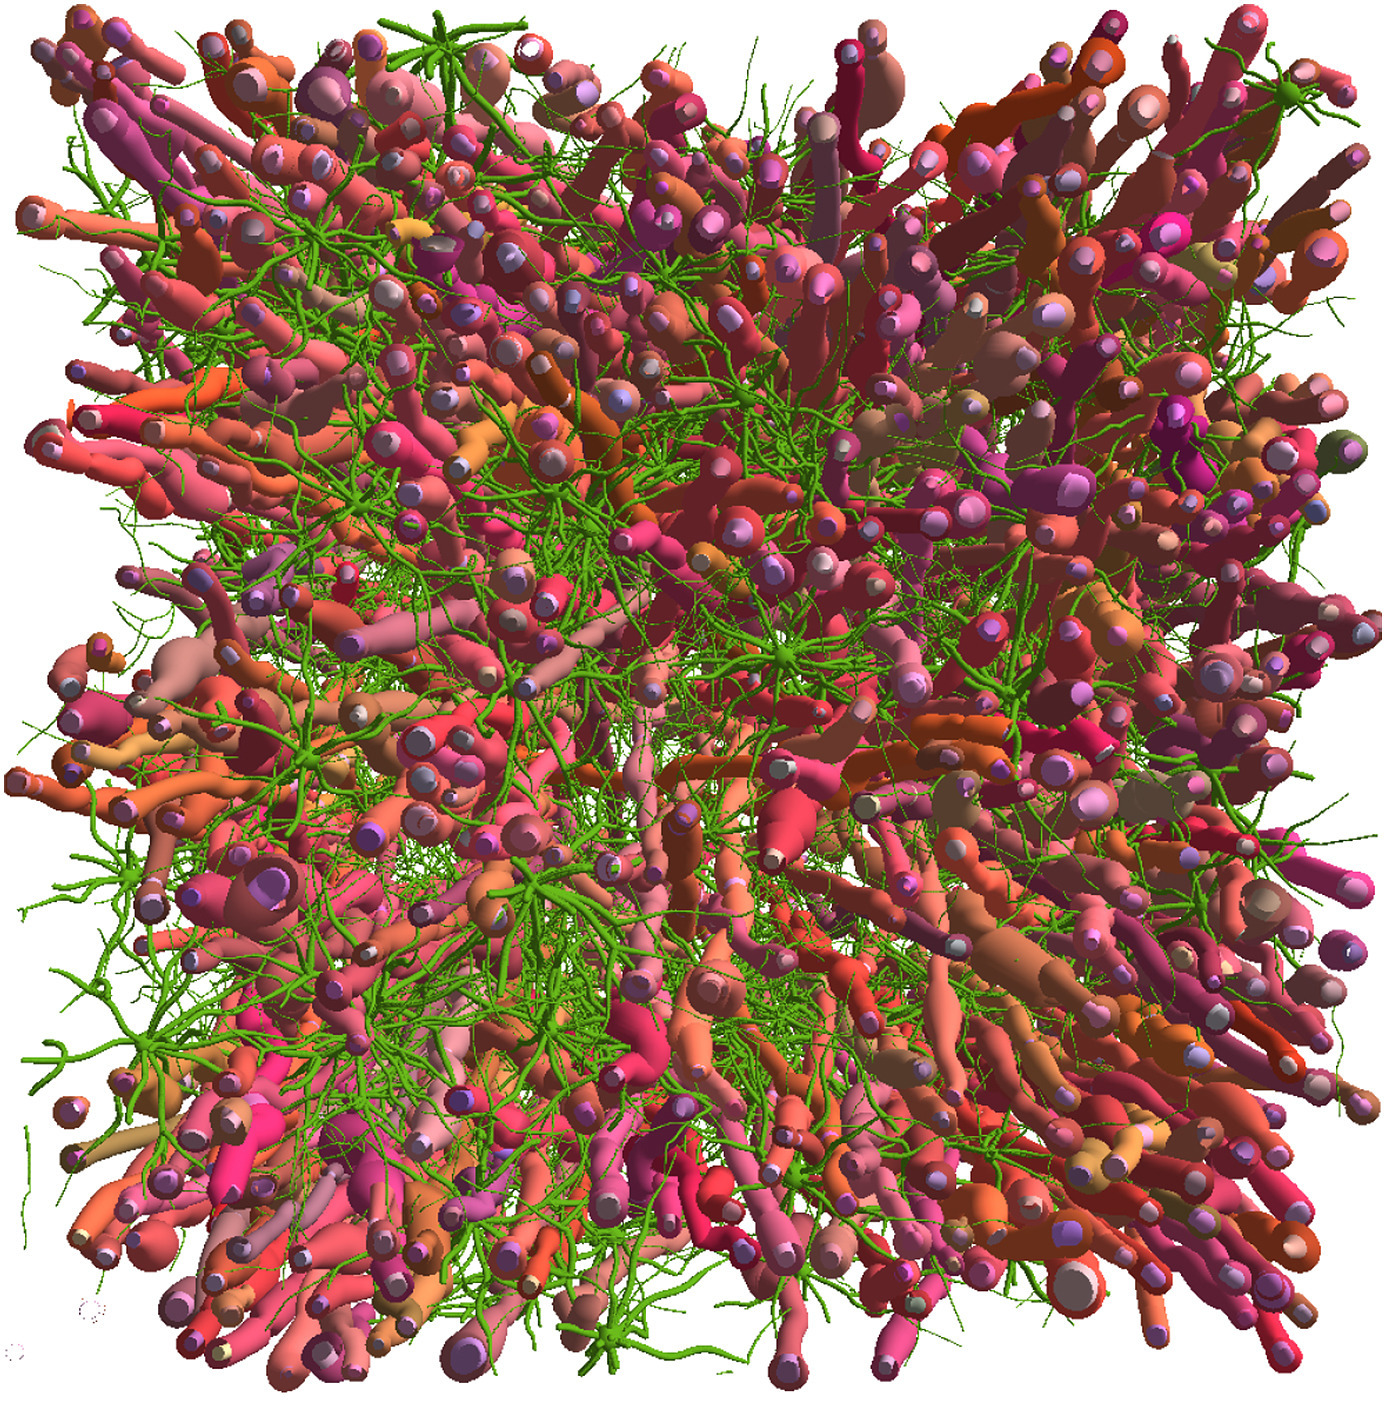
\includegraphics{gfx/model/medusa/11_.jpg}}}
	\caption{\cite{Ginsburger2019}}
	\label{fig:medusa_8}
\end{figure}
% 
%
\cleardoublepage
\setcounter{chapter}{4}
\chapter{\acs{3D-PLI} simulation}
\label{cha:sof:simulation}
%
In the past simulation of \ac{3D-PLI} already shown their capabilities \cite{Dohmen2015,Menzel2015,Menzel2016,Menzel2020,Menzel2021,MenzelMaster,MenzelDissertation}.
In the case of scattering finite-difference time-domain simulations the here presented algorithm to design new collision free fiber models allowed for the first time to simulate the effect of scattering light without any superposed interference signals.
This allowed the understanding of scattering effects due to the configurations of fiber bundles and crossings as well as the transmittance change for inclined fiber configurations.\cite{MenzelDissertation,Menzel2020,Menzel2021}.
\par
% 
In the case of the simulation of linear optics the optical system could repoduse the experimental results with \eg{} the optical resampling process \cite{Dohmen2015,Menzel2016}.
However this algorithm is very computational heavy and due to the precalculations of a discretised tissue volume, very memory intense.
The foundations of a more efficient parallel algorithm for the use of supercomputer was already elaborated \cite{Lucksch2016}.
However, the new tilting design resulted in a simplification of the former simulation that could not be easily integrated.
Therefore the algorithm was completely redesigned and rewritten.
Additionally the here presented fiber models had to be Incorporated as well.
Finally the descision was made, to switch to the M\"{u}ller Stokes calculus to allow also account for polarization effects of filters.
\par
%
The Simulation is split into two consecutive parts: the volume discretizer and the simulation.
The volume discretizer discretises the virtual nerve fiber models onto a cartesian grid, which is then in the second step used to calculate the light matter interaction.
One parallelization technique allows to split the volume onto different \acp{CPU} or nodes.
Due to the tilting approach, the light vector needed to be able to leave the current volume of a single \ac{CPU} and traverse to the next volume/\ac{CPU}.
This simulation as well as the optical characterization of the system and the inclination analysis will be discussed here.
\\
%
The code is as the former written in \cpp{} with a user friendly wrapper function in \python{}.
%
% 
% 
\section{Discrete volume generator}
\label{sec:dv_generator}
%
\begin{figure}[!t]
\centering
\setlength{\tikzwidth}{0.5\textwidth}
\inputtikz{gfx/simpli/disc_volume}
\caption[discreticed tissue volume]{Discretized tissue volume: Its boundry is defined by a \ac{AABB}, which itself is defined by the lower and upper corner values $v_\mathit{min}$ and $v_\mathit{max}$. \todo{show x,y,z resulting volume?}\todo{show fiber model inside?}}
\label{fig:discVol}
\end{figure}
%
The idea of the simulation is to split the necesarry calculation in to conesqutive parts. The first one is to calculate a discretised tissue volume.
It represents a discrete constant voxel model of the tissue.
This helps to drastically speed up the light matter interaction of the next step (see \cref{sec:simulation}).
\par
%
The discreticed tissue volume represents a cuboid sliced into equal sized smaller cubes called voxels, \ie 3d pixels (see \cref{fig:discVol}).
Each voxel contains the physical properties of the tissue inside its current position.
The overall volume is limited by an \ac{AABB} or \ac{VOI}, which is defined by a minimal and maximal value $\voi = [(x_{\mathit{min}}, y_{\mathit{min}}, z_{\mathit{min}}),(x_{\mathit{max}}, y_{\mathit{max}}, z_{\mathit{max}})]$.
Additionally the \voxelsize{} parameter \voxels{} is set to a floating point number and defines the edge length of the voxels.
If the division of the \voi{} by the \voxelsize{} is not an integer, the \voi{} is automatically increased to the next possible integer value to avoid boundary effects.
%
%
%
\subsection{Nerve fiber layers}
%
As described in \cref{sec:fiberArchitecture} nerve fibers are axons, which can be wrapped around by several windings of myelin (see \cref{fig:fiberLayer}).
Especially for light wave simulations the myelin windings are a significant property \cite{MenzelDissertation}.
This makes it necessary to be able to build such a structure.
\par
%
An easy implementation is to represent the windings as layers (see \cref{fig:myelinLayer}).
This simplifies the creation process significantly.
A layer can then simply defined by a factor between $0$ and $1$, which scales with the nerve fiber radius.
For example, $0.75$ means that from $0 \leq r < 0.75$ of the radii are interpreted as the first layer.
\par
%
Each layer needs to its radius also a set of physical properties:
%
\begin{itemize}[nosep]
    \item birefringence value $\dn$
    \item absorption coefficient $\mu$
    \item optical axsis model $p=\mathit{parallel}$, $r=\mathit{radial}$, $b=\mathit{background}$
\end{itemize}
%
These properties are set as a list of tuples inside the algorithm (see \cref{alg:fiberbundleprops}).
%
\begin{lstfloat}[!ht]
\lstset{style=python}
\begin{lstlisting}[]
fbs_properties = [[(r, dn, mu, 'p'), (second layer), ...],
                  [(first layer of second bundle), ...],
                  [...]]
\end{lstlisting}
\caption[Fiber bundle properties]{Defining fiber bundle properties.}
\label{alg:fiberbundleprops}
\end{lstfloat}
%
At the end the DV-Generator returns the arrays \tissue{}, \opticalaxis{} and the \propertylist{} for the use of the simulation.
%
\subsection{Discretizing a nerve fiber model}
%
\begin{figure}[!t]
\centering
\setlength{\tikzwidth}{0.32\textwidth}
\subcaptionbox{\label{fig:myelinLayer}Schematic of nerve fiber with axon and wrapped around myelin}[.32\textwidth]{
\includegraphics[height=0.3\textwidth]{dev/brain/myelin_layers.pdf}\vspace{0mm}}\hfill
\subcaptionbox{\label{fig:fiberLayer}Cross section nerve fiber with layered structure definde by $n$ radii}[.32\textwidth]{
\inputtikz{gfx/simpli/fiber_layer}\vspace{-5mm}}\hfill
\subcaptionbox{\label{fig:vectormodel}Cross section of discreticed nerve fiber with resulting vectors of optical axis}[.32\textwidth]{
\inputtikz{gfx/simpli/vector_model}\vspace{-5mm}}
\caption{Discretisation of nerve fiber with layered structure.}
\label{fig:fiber_discretisation}
\end{figure}
%
To discretize nerve fiber models (see \cref{chap:sof:modelling}) one can start with the discretization of a single nerve fiber segment, since a fiber is a chain of consecutive segment.
The idea is, that if a voxel is inside a fiber segment, it will be marked as a tissue with the physical properties (absorption, optical axis and birefringece) from the voxels center position $\vec{q}$ (see \cref{fig:fiber_discretisation}).
In this context \say{a voxel inside a fiber segment} means, that its center point is inside the volume of the fiber segment.
The discretized tissue is designed in such a way that, that the arrays position $[i,j,k]$ takes up the space of $(i,j,k)$ to $(i+1,j+1,k+1)$ in the unit of \voxelsize{}.
\par
%
Therefore the filling process can be integrated by looping over all voxels in the current volume.
However since a single nerve fiber segment is usually much smaller than the volume, it makes sense to reduce the size of the iterating voxels.
This is easily be done by only iterating over the voxels of the \ac{AABB} of the nerve fiber segment.
\par
%
Now each voxel will be checked, if it is inside the nerve fiber segment.
This is analog calculated to the collision between two nerve fiber segment (see \cref{alg:pseudocodeCollisionDetection}) except that only one point of the closest distance has to be found.
The other one is the voxels center position $\vec{q}$.
From this calculation not only the closest points $\vec{p}_a$ and $\vec{p}_b$ will be returned, but also the distance vector $\vec{d}$.
This helps to calculate the the distance, which will be used to check if the voxel is inside the fiber segment, and if it is, in wich layer of the fiber segment it is.
Additionally the distance vector calculation $\vec{d}$ is used, if the optical axis inside the current layer is set to a microscopic model. Then the optical axis is orientated radial to the fiber segment. This orientation is identical to calculate the minimal distance from that current point to the line segment.
\par
%
Two values have to be stored in the case of a valid entry.
The first one is an index inside a \code{tissue} array, which is later used to retreve the properties from a list with the same index order.
The second one is the orientation of the optical axis inside the current layer.
The orientation is either parallel to the fiber segment in case of the macroscopic model, or radial in the case of the microscopic model.
A layer can also be marked as \say{background}, which will allow the user to specify a region with absorption, but without a birefringence.
\par
%
Before looping over all fiber segments, an additional problem has to be solved.
Since two consecutive fiber segments will take up the same space because they share a point, they also will fill the voxel of the tissue volume.
This is a problem, since now the second fiber segment will overwrite the values of the first one.
This can easily be solved by adding an additional array, which will store the smallest distance inside, which was calculated when filling the voxels space.
The values will now be overwritten, if a new smallest distance was calculated, which is smaller then the already stored one.
This also solves the problem, that at the end end points of a fiber segment in the case of a radial optical axis model, the optical axis would be \say{star like}.
This of course will still be the same at the beginning and end of an fiber.
\par
%
This \say{filling} loop is represented in the pseudocode \cref{alg:fillVolume}.
%
\begin{lstfloat}[!tb]
\lstset{style=python}
\begin{lstlisting}[]
for fiber_segment in fiber_bundle:
    for i,j,k in fiber_segment.aabb().voxels():
        min_dist, min_point = calculate_min_distance((i,j,k), cc)
        if min_dist < cc.radius:
            if min_dist < current_distance[i,j,k]:
                optical_axis[i,j,k,:] = get_axis_orientation(
                                            (i,j,k), min_dist,
                                            min_point)
                tissue[i,j,k] = get_layer_id(min_dist)
                current_distance[i,j,k] = min_dist
\end{lstlisting}
\caption{Discretized volume filling algorithm}
\label{alg:fillVolume}
\end{lstfloat}
%
The length of the optical axis vector is interpreted as strength. In this model the length is usualy always 1. If the user wishes to add variability, one can do this by changing the length of the vectors inside the arrays.
%
%
%
\subsection{\voxelsize}
%
\begin{figure}[!t]
\centering
% \tikzset{external/export=false}
\setlength{\tikzwidth}{.24\textwidth}
\definecolor{c1}{rgb}{0.25,0.4,0.1}
\definecolor{c2}{rgb}{1.0,0.73,0}
\definecolor{c3}{rgb}{0.98,0.4,0.25}
\definecolor{c4}{rgb}{0.22,0.36,0.59}
%
% \definecolor{c1}{HTML}{440154FF}
% \definecolor{c2}{HTML}{38598CFF}
% \definecolor{c3}{HTML}{1E9B8AFF}
% \definecolor{c4}{HTML}{FDE725FF}
%
\def\xc{0.7}
\def\yc{0.2}
\def\rin{1.5}
\def\rout{3}
%
% 
\newcommand{\fiber}[3]{
	\def\dd{#1}
	\pgfmathsetmacro{\xmin}{int(floor(\xc-\rout))}
	\pgfmathsetmacro{\xmax}{int(ceil(\xc+\rout))}
	\pgfmathsetmacro{\xd}{\xmin+\dd}
	\pgfmathsetmacro{\ymin}{int(floor(\yc-\rout))}
	\pgfmathsetmacro{\ymax}{int(ceil(\yc+\rout))}
	\pgfmathsetmacro{\yd}{\ymin+\dd}
	%
	\pgfmathsetmacro{\rmin}{\rin*\rin*100}
	\pgfmathsetmacro{\rmax}{\rout*\rout*100}
	\foreach \x in {\xmin,\xd,...,\xmax} {
		\foreach \y in {\ymin,\yd,...,\ymax} {
			\pgfmathsetmacro{\d}{int(((\x-\xc+\dd/2)*(\x-\xc+\dd/2)+(\y-\yc+\dd/2)*(\y-\yc+\dd/2))*100)}
			\ifnum\d>\rmin
			\ifnum\d<\rmax
			\path [#3] (\x,\y) rectangle ($ (\x, \y) + (\dd, \dd) $);
			\draw[#2] ($ (\x, \y) + (0, 0) $) -- ($ (\x, \y) + (\dd, 0) $);
			\draw[#2] ($ (\x, \y) + (\dd, 0) $) -- ($ (\x, \y) + (\dd, \dd) $);
			\draw[#2] ($ (\x, \y) + (\dd, \dd) $) -- ($ (\x, \y) + (0, \dd) $);
			\draw[#2] ($ (\x, \y) + (0, \dd) $) -- ($ (\x, \y) + (0, 0) $);
			\fi\fi
		}
	}
%	\foreach \x in {\xmin,\xd,...,\xmax} {
%		\draw[#2] (\x,\ymin) -- (\x,\ymax);
%	}
%	\foreach \y in {\ymin,\yd,...,\ymax} {
%		\draw[#2] (\xmin,\y) -- (\xmax,\y);
%	}
}
%
\subcaptionbox{}[\tikzwidth]{
\resizebox{\tikzwidth}{!}{
\begin{tikzpicture}[]
\path[] (-3.75, -3.5) rectangle (3.75, 3.25);
\begin{scope}[shift={(-\xc,-\yc)}]
\fiber{2}{line width = 0.2mm}{pattern color=c1,pattern=horizontal lines}
\draw[line width = 0.4mm] (\xc,\yc) circle (\rin);
\draw[line width = 0.4mm] (\xc,\yc) circle (\rout);
\end{scope}
\end{tikzpicture}
}}
\hfill
%
\subcaptionbox{}[\tikzwidth]{
\resizebox{\tikzwidth}{!}{
\begin{tikzpicture}[]
\path[] (-3.75, -3.5) rectangle (3.75, 3.25);
\begin{scope}[shift={(-\xc,-\yc)}]
\fiber{1}{line width = 0.1mm}{pattern color=c2,pattern=vertical lines}
\draw[line width = 0.4mm] (\xc,\yc) circle (\rin);
\draw[line width = 0.4mm] (\xc,\yc) circle (\rout);
\end{scope}
\end{tikzpicture}
}}
\hfill
%
\subcaptionbox{}[\tikzwidth]{
\resizebox{\tikzwidth}{!}{
\begin{tikzpicture}[]
\path[] (-3.75, -3.5) rectangle (3.75, 3.25);
\begin{scope}[shift={(-\xc,-\yc)}]
\fiber{0.5}{line width = 0.05mm}{pattern color=c3,pattern=north east lines}
\draw[line width = 0.4mm] (\xc,\yc) circle (\rin);
\draw[line width = 0.4mm] (\xc,\yc) circle (\rout);
\end{scope}
\end{tikzpicture}
}}
\hfill
%
\subcaptionbox{}[\tikzwidth]{
\resizebox{\tikzwidth}{!}{
\begin{tikzpicture}[]
\path[] (-3.75, -3.5) rectangle (3.75, 3.25);
\begin{scope}[shift={(-\xc,-\yc)}]
\fiber{0.25}{line width = 0.025mm}{pattern color=c4,pattern=crosshatch dots}
\draw[line width = 0.4mm] (\xc,\yc) circle (\rin);
\draw[line width = 0.4mm] (\xc,\yc) circle (\rout);
\end{scope}
% \fiber{2}{}{fill, c1, opacity=0.25}
% \fiber{1}{very thin}{fill, c2, opacity=0.25}
% \fiber{0.5}{ultra thin}{fill, c3, opacity=0.25}
% \fiber{0.25}{ultra thin}{fill, c4, opacity=0.25}
%
\end{tikzpicture}
}}
\caption[Discretization error]{Discretization error. Cross section of single fiber with one myelin layer inside discretized tissue volume. The couloured pattern show the resulting voxels which corresponds to the fiber. The smaller the \voxelsize{}, the smaller the representation error.}
\label{fig:vectorfield_disc_error}
\end{figure}
%
The \voxelsize{} parameter is the most important property of the simulation.
It will determine, how accurate the simulation is.
This is first of all because it will change the number of voxels with which the nerve fiber model is discretized (see \cref{fig:vectorfield_disc_error}).
Especially for the case of multiple layers this will have an major impact.
Additionally it will also change the \stepsize{} of the light through the tissue.
Usually the \stepsize{} is the same as the \voxelsize{}, but the user can change it if necessary.
Also the number of light particels will increase with decreasing \voxelsize{} since for about each voxel at the bottom of the tissue a single light particle will be casted (see \cref{sec:pathOfLight}).
Therefore the resulting intensity signal will also be more accurate.
%
%
% 
\subsection{optimization}\label{sec:dvOpti}
%
All arrays are implemented as contiguous c-arrays, which are accessible as \name{Numpy}-arrays from outside without the need to copy the data.
Since these arrays grow with $\mathcal{O}(n^3)$, the aim was to make them movable through the \cpp{} libraries as well as in \python{}.
The memory order of the arrays is in $x\text{-}y\text{-}z$ direction, so the largest memory shift is in $x$ and the smallest in $z$.
This was chosen so that later in the simulation part, where the light travels mainly in $z$-direction, the memory is aligned to the required information and thus the \acp{CPU} cache prefetcher can be used.
\par
%
Two methods are used to parallelize the algorithm on the \ac{CPU}.
The first uses \ac{OpenMP} to parallelize the filling of the \ac{AABB} volume of each object.
The second uses \ac{MPI} to allow distribution to multiple \ac{CPU} cores without sharing memory (detailed description in \cref{sec:mpiSim}).
\par
%
The parallelization of filling the voxels of the discretized volume leads to a race condition if several threads want to write or read to the same memory address (or coordinate) (\eg{} two objects occupy the same space).
A solution with a lock would be very slow since, depending on the fiber segment length and orientation, most voxels of the \ac{AABB} have to be written to.
Also since many of the voxels don't need to be overwritten, most locks would be unnecessary.
\\
Since the loop runs over all $(i,j,k)$ indices of the three space dimensions, the parallelization can be done using the iteration over the voxels themself per fiber segment.
However, this leads to a slow implementation because new threads have to be spawn for each fiber segment, which takes quite some time.
If was therefore decided, that the parallel call creates all threads before the first loop over all objects.
This means all threads process all objects.
If the threads then execute a loop over all indices (or coordinates), thread $n$ only processes the memory for the first volume dimension $i$ if (see \cref{fig:discVolThread}):
%
\begin{figure}[!t]
\centering
\setlength{\tikzwidth}{0.5\textwidth}
\inputtikz{gfx/simpli/disc_volume_thread}
\caption[discretized volume parallelization]{discretisation volume parallelization with \ac{OpenMP}. Each thread handles every n-th yz-section. This ensures both thread safety and that the workload is more balanced, even with an inhomogeneous.}
\label{fig:discVolThread}
\end{figure}
%
\begin{align}
\begin{split}
    i \bmod N_{\mathit{Threads}} == \mathit{thread}_{\mathit{id}}
\end{split}
\end{align}
%
This process results in a thread-safe writable operation.
The only drawback is that all threads must check if the \ac{AABB} is inside the \ac{VOI}.
However since with this configuration only once threads are spawned, and the \ac{AABB} collison check is very efficient in terms of computation time, it is quite fast.
Additionally the shared cache of the \acp{CPU} can speed up the memory retrieving process as well, if the \acp{CPU} workload do not differ that much.
\par
\paragraph{Note}
Depending on the size of the volume and the acessable memory, the user is adviced to distribute the \ac{OpenMP} parallelization on one node and the \ac{MPI} distribution on multiple nodes. Depending onthe Architecture the distribution is not straightforword to optimize. Individual tests should be performed.
The \ac{OpenMP} speedup is usually as fastest if the spawend threads are located on the same physical \ac{CPU} or even inside the same \acp{CPU} which uses the same cache.
It can therefore be that the speedup is increased by reducing the \ac{OpenMP} threads and by increasing the \ac{MPI} threads instead.
%
%
%
\section{Simulation}
\label{sec:simulation}
%
The simulation algorithm executes the M\"uller-Stokes calculus (see \cref{sec:Mueller-Stokes}) on the previously calculated discrete volume (see \cref{sec:dv_generator}) for a light beam along its path.
Since no scattering or refraction effects are included in this simulation, each light path follows a straight line.
The interaction of light matter is calculated according to $\left( \prod_i R_i M_i R_i \cdot \vec{S} \right)$ (see \cref{sec:mueller_stokes}).
Befor the light vector is multiplied by the polarizer of the optical system.
After the light beam has reached the end of the tissue, the last optical elements are taken into account.
Finally, the light intensity is stored in the \acs{CCD} image array, which has at this point the same size as the 2d $xy$-grid of the discretized tissue.
At the end it will be resampled to the final \ac{CCD} array size and a noise model will be applied.
%
%
\subsection{Path of light}
\label{sec:pathOfLight}
%
\begin{figure}[!t]
\setlength{\tikzheight}{0.42\textwidth}
\subcaptionbox{camera view}[.49\textwidth]{
\inputtikz{gfx/simpli/tilting_3d_a}}\hfill
\subcaptionbox{perspective view}[.49\textwidth]{
\inputtikz{gfx/simpli/tilting_3d_b}}
\tikzset{external/export=false}
\caption[3d tilting]{3d tilting: around $xy$-axis, \raisebox{.25em}{\tikz \draw[red,thick](0,0)--(0.25,0);} top, \raisebox{.25em}{\tikz \draw[green,thick](0,0)--(0.25,0);} middle, \raisebox{.25em}{\tikz \draw[blue,thick](0,0)--(0.25,0);} bottom, \raisebox{.25em}{\tikz \draw[dash pattern=on 1.25pt off 1.25pt,thick](0,0)--(0.25,0);} original, \raisebox{.25em}{\tikz \draw[gray](0,0)--(0.25,0);} axis of rotation.}
\label{fig:tilting_camera_view}
\end{figure}
%
The simulation allows a tiltable light beam.
For this purpose, the \ac{LAP} uses a tilting stage to which the tissue sections are attached (see \cref{fig:tilted_side_view}).
The newly designed microscope on the other hand has a already tilted light beams.
There are generated by an conical light path, from which then with an aperture the desired light orientation is sampled (see \cite{Wiese:887678}).
Both methods yield within a good approximation to the same light paths.
\\
%
The tilting can lead to a distortion of the image (see \cref{fig:tilting_camera_view}).
This distortion can be described by an affine transformation (see \cref{fig::affine_transformation}):
%
\begin{figure}[!t]
\centering
\pgfmathsetmacro{\size}{10}
% 
\subcaptionbox{}[.225\textwidth]{
\resizebox{.225\textwidth}{!}{
\begin{tikzpicture}[]
\pgfmathsetmacro{\dx}{2.25}
\pgfmathsetmacro{\dy}{1.5}
\draw[help lines] (0,0) grid (\size,\size);
\foreach \i in {0,...,\size}{
	\draw [very thick] (\i+\dx, 0+\dy) -- (\i+\dx, \size+\dy);
	\draw [very thick] (0+\dx, \i+\dy) -- (\size+\dx, \i+\dy);
}
\end{tikzpicture}
}}
% 
\subcaptionbox{}[.225\textwidth]{
\resizebox{.225\textwidth}{!}{
\begin{tikzpicture}[]
\pgfmathsetmacro{\sx}{1.5}
\pgfmathsetmacro{\sy}{0.75}
\draw[help lines] (0,0) grid (\size,\size);
\foreach \i in {0,...,\size}{
	\draw [very thick] ({\i*\sx}, 0) -- ({\i*\sx}, {\size*\sy});
	\draw [very thick] (0, {\i*\sy}) -- ({\size*\sx}, {\i*\sy});
}
\end{tikzpicture}
}}
%
\subcaptionbox{}[.225\textwidth]{
\resizebox{.225\textwidth}{!}{
\begin{tikzpicture}[]
\draw[help lines] (0,0) grid (\size,\size);
\begin{scope}[rotate around={30:(0.5*\size,0.5*\size)}]
\foreach \i in {0,...,\size}{
	\draw [very thick] (\i, 0) -- (\i, \size);
	\draw [very thick] (0, \i) -- (\size, \i);
}
\end{scope}
\end{tikzpicture}
}}
% 
\subcaptionbox{}[.225\textwidth]{
\resizebox{.225\textwidth}{!}{
\begin{tikzpicture}[]
\pgfmathsetmacro{\cx}{0.5}
\pgfmathsetmacro{\cy}{0}
\draw[help lines] (0,0) grid (\size,\size);
\foreach \i in {0,...,\size}{
	\draw [very thick] (\i+0*\cx, 0+\i*\cy) -- (\i+\size*\cx, \size+\i*\cy);
	\draw [very thick] (0+\i*\cx, \i+0*\cy) -- (\size+\i*\cx, \i+\size*\cy);
}
\end{tikzpicture}
}}
\caption{affine transformation}
\label{fig::affine_transformation}
\end{figure}
%
\begin{align}
f(\vec{x}) = \mat{A} \cdot \vec{x} + \vec{t}
\end{align}
where $\vec{x}$ the coordinate input, $\mat{A}$ and $\vec{t}$ the transformation values and $f(\vec{x}$ the transformed coordinate.
\\
%
The simulation is able to take the distorted view into account and it can resample the starting positions of the light beams such, that the distortion is reversed.
It is the same as distorting the \ac{CCD} sensor, however without the need of interpolation of the \ac{CCD} image sensor.
In the case of simulating the distortion, the affine inverse transformation $f^{-1}(\vec{x}) = \mat{A}^{-1} \cdot \vec{x} - \vec{t}$ can be applied.
However, this leads to interpolation artifacts.
Therefore both techniques exists to be able to study this effect in more detail.
\par
%
An additional effect is the simulation of the refraction of the tissue-air border, which is described by Snell's law for isotropic media (see \cref{eq:Snellius})
Since this only adds a parallel shift, a simulation is only necessary if the resampling of an image registration is to be studied.
\par
%
\begin{figure}[!t]
\setlength{\tikzwidth}{0.42\textwidth}
\subcaptionbox{normal}[.495\textwidth]{
\def\tilt{0}
\def\nindex{2.25}
\inputtikz{gfx/simpli/tilting_a}}\hfill
\subcaptionbox{tilted}[.495\textwidth]{
\inputtikz{gfx/simpli/tilting_b}}
\caption[Light path]{Ligh path for a normal (a) and tilted (b) case. For the tilted case the light beam $\vec{l}_1$ gets tilted inside the tissue and therefore recieves a optical shift $\Delta$.}
\label{fig:tilted_side_view}
\end{figure}
%
The starting position of the light beam can be calculating by traversing the light path backwards (see \cref{fig:tilted_side_view}).
Each light beam $\vec{l}_0$ hitting the \ac{CCD}-array element, not resampled yet to the actual \ac{CCD} pixel size, can be traversed back to the tissue top plane $\mathfrak{S}_{top}$.
Next the light beam $\vec{l}_1$ is traversed back through the tissue to the bottom plane $\mathfrak{S}_{bottom}$.
The point on the bottom tissue plane corresponds to the starting position of the light beam.
In the case of a tilted light beam or lilted tissue, a offset of $\Delta$ is occurs.
The backtracking of the light from the ccd-array to the tissue is prevends a  resampling process and therefore no boarder effects can occurs.
\\
%
In the case of already simulating an undistored view, the light paths have to spaced out by the same distance, as the affine transformation would resample the resulting pixels.
%
\begin{lstfloat}[!p]
	\lstinputlisting[style=cpp,basicstyle=\scriptsize\ttfamily,]{code/simulation.cpp}
	\caption{Pseudocode simulation \todo{anhang}}
	\label{alg:simulation}
\end{lstfloat}
%
\subsection{Tissue voxel interpolation}
%
For a \stepsize{} unequal to the \voxelsize{} or a tilted light path the midpoint does not match the center point of the voxel anymore.
This means, that the physical properties stored in the arrays have to be interpolated.
%
\begin{figure}[!t]
\centering
\setlength{\tikzwidth}{0.45\textwidth}
% \tikzset{external/force remake=true}
\subcaptionbox{\label{fig:triInterp}Trilinear interpolation}[\tikzwidth]{
\hfill\inputtikz{gfx/simpli/trilinear_interpolation}\hfill}\hfill
\subcaptionbox{\label{fig:sphInterp}Spherical interpolation}[\tikzwidth]{
\inputtikz{gfx/simpli/vector_interpolation}}
\caption[]{Interpolation techniques: The trilinear interpolation can be visualized as a axial step interpolation. The difference between linear and spherical interpolation is that the linear interpolation has a constant distance $s$ between each point while the spherical interpolation has a constant angle $\varphi$ for the same step.}
\label{fig:vectorfield_disc}
\end{figure}
%
There are currently three interpolation methods for this purpose implemented: \textit{nearest neighbor}, \textit{linear interpolation} and \textit{spherical interpolation}.
The voxels taken into account for the interpolation are the nearest 8 adjacent voxels, so array indices $(\floor{x\pm0.5},\floor{y\pm0.5},\floor{y\pm0.5})$.
%
The \textit{nearest neighbor} is the most error-prone of the three methods and should be not to be used.
However it is also the fastest method.
The \textit{linear interpolation} was the first one implemented.
However since the data contain orientation data, the \textit{spherical interpolation} method should be used.
\\
%
To interpolate the data the trilinear interpolation will be performed (see \cref{fig:triInterp}).
%
%
%
\subsection{algorithm}
%
First the starting points of all light beams will be calculated.
hen each light beam can be traversed inside the tissue.
To calculate the light matter interaction, the change of the Stokes vector will be calculated after each light beam step.
As soon as the light hits the boarder of the tissue, the light beam will be the last optical elements and the intensity will be stored inside the \ac{CCD} array.
The pseudocode is shown in \cref{alg:simulationLoop}.
%
\begin{lstfloat}[!tb]
\lstset{style=python}
\begin{lstlisting}[]
light_beams = calculate_light_starting_positions()

for light in light_beams:
    light = optical_elemts_start * light
    while light.pos in volume:
        properties = get_properties(light.pos)
        light.intensity *= exp(-step_size * properties.absorbtion)
        light = matrix(properties) * light
        light.pos += step_size
   
    light = optical_elemts_end * light
    ccd_array[light.ccd_pos] = light.intensity
\end{lstlisting}
\caption{Discretized volume filling algorithm}
\label{alg:simulationLoop}
\end{lstfloat}
%
%
%
\subsection{Optimizations}
%
There are several optimizations used inside this pipeline.
First the order of the tissue stored inside the memory is along the z-axis (as described in \cref{sec:dvOpti}).
Secondly the main for loop for each light ray is parallized with \ac{OpenMP}.
This threads are completely separated and no race conditions exists.
%
%
%
\subsection{Optic}
\label{sec:ccdOptic}
%
The image sensor as described in \cref{sec:expSetup} is a \ac{CCD} sensor.
The calculations, \ie the resampling and noise modelling, are implemented according to \cref{sec:opticalResolution}.
These calculations are performed on the python side of the algorithm and can be parallized with the \code{multiprocessing} library of \python{}.
%
% A general \ac{CCD} sensor consits out of an array of capacitors.
% In each capacitor an electric charge will be stored, setted free by an incoming photons.
% After a read out process, which also contains a electric gain, the resulting values can be stored as an image.
% This process has two major noise parts. The first is the electic charge.
% Its value is, as long as it is not saturated, linear correlated with the number of photons.
% However internal noise like thermal, and a each photon statistically charges a number of electrons, the resulting capacity varies.
% The second major noise comes from the gain process.
% Here the electric voltage will be gained before a analog digital read out.
% This process is also strong linear correlated around a operational point.
% However due to the nature of the underlining circuit, i.e. usually transistors and their power source, the resulting value can vary.
% All noise sources combined yield to an poison distributed noise, to too the nature of digital values.
%
% \\
%
% To account for the optical setup, three things have to be done.
% \paragraph{Bluring}
% The optical resolution the light rays have to be blurred.
% This is classically done via a 2d gaussian convolution:
%
% \paragraph{Sampling}
% Since the number and final position of the light rays is according to the voxels, all intensities of an image pixel have to be combined.
% Here it is done via a mean value sampling.
% This in contrast to resizing, does not interpolates the image.
% %
% \paragraph{Noise}
% The last step is to replicate the noise of the image setup. To account for this a noise model has to be applied to each image pixel. \cite{Wiese:887678} showed that this can be done via a poisson/gaus model.
%
%
%
\section{Analysis}
%
The same algorithms are implemented as in the \ac{3D-PLI} routine pipeline (see \cref{sec::intSignal,sec::InclAnalysis}).
This include the modalities analysis transmittance, direction and retardatation as well as the tilting analysis performend by \ac{ROFL}.
%
%
%
\section{MPI parallelization}\label{sec:mpiSim}
%
Both algorithms, the DV generator and the simulation can use an additionally parallelization technique.
%
For huge volumes that are larger than the locally memory size, the calculation must be split onto several physical \acp{CPU} and \name{computation nodes}\footnote{A computing node is a processing unit in a computer network}.
For this purpose \acreset{MPI} \ac{MPI} is used.
A method is implemented that automatically divides the volume along the $x$-axis and $y$-axis into blocks with minimal surface area (see \cref{fig:com_halo}).
The minimization of the $x-y$-surface area is important for the simulation algorithm.
\\
Once the volume is split into euqal parts, with respect to the nature of integers, the above mentioned algorithms can be performend completly analog on the \ac{MPI} ranks, as if they only would know about there volume.
The only exception is the simulation for tilted light beams.
This means, that at the boarder of the volume, when a light beam travels through the tissue, the light can leave the local volume of the \ac{MPI} rank.
\ac{MPI} provides several methods to send information to another rank.
Since this volume splitting is cartesion, the cartesion implementations of \ac{MPI} are used (\eg{} \code{MPI\tu Cart\tu create}).
However since the light beam also needs in the case of interpolation the information of the surrounding $\SI{8}{\voxel}$, this would mean that the missing voxels had to be transferred to the neighboring ranks.
%
\begin{figure}[!t]
\centering
\setlength{\tikzwidth}{0.85\textwidth}
\inputtikz{gfx/simpli/com_halo}
\caption{comunication halos. The volume is split into six subvolumes, distributed to 6 mpi ranks. The coloured voxels have the same tissue information.  To calculate the value at a given point a eight-neighborhood is necessary.}
\label{fig:com_halo}
\end{figure}
%
This would mean a huge amount of communications, which are relatively slow.
The solution is a so called \name{halo}.
This is a commonly used concept, where the borders (in this case a volume) are enlarged by a a specific size (in this case $\SI{1}{\voxel}$) so that the same information of the shared regions is available everywhere (see \cref{fig:com_halo}).
%
% \begin{figure}[!t]
% \centering
% \def\tikzwidth{0.5\textwidth}
% \inputtikz[]{gfx/simpli/com_halo_send}
% \caption{Light ray send to another node. To calculate the \dummy{} a eight-neighborhood is necessary.}
% \label{fig:com_halo_light}
% \end{figure}
Now the light beam can be communicated when it leaves the local volume to the next one (see \cref{fig:com_halo}).
This is also the reason, why the surface area is minimized, so that the number of communications is also minimized.
\\
To even more speed up the communication process, all leaving light beams are first stored locally in a communication buffer, and only after all local light beams were processed, the buffer will be communicated to the neighbors.
This ensure a minimal communication cost.
The main light beam algorithm loop is then started again on all \ac{MPI} ranks for the communicated light beams.
This is repeated until no more communications were necessary.
\par
%
Each \ac{MPI} process can additionally use \ac{OpenMP} to create multiple threads for efficient use of shared memory if the architecture supports it.
% 
%
%
\cleardoublepage
\cleardoublepage
\setcounter{chapter}{5}
\chapter{\acs{fastPLI}}
\label{chap:Software}
% 
% 
% 
\section{Introduction}\label{sec:fastpliIntro}
%
The previous chapters described the algorithms for creating dense \ac{WM} fiber models (see \cref{chap:sof:modeling}) and for simulating such models in \ac{3D-PLI} (see \cref{cha:sof:simulation}).
Both algorithms are designed to operate autonomously without knowledge of the other.
This can simplify the use of the algorithms for other domains. For example, the fiber models can be used in other in the field of \ac{dMRI} as well (\cite{Ginsburger2019,ginsburgerDis2019}).
However, besides providing algorithms that should be very fast and therefore in this case at a very low level of the programming language (very few abstractions), it is also necessary to provide an API that provides an interface for the user.
This interface must be designed in such a way that the user has a good experience with the algorithms.
Among other things, this means a high level of abstraction with logical and easy-to-use naming systems.
A high level of abstraction in software design means eliminating unnecessary systems and generalizations of functionalities.
\par
%
In addition, the algorithms should be accessible to a wide audience.
Among other things, this means that the program must be installable and easy to understand, even if hardly any programming knowledge is available.
The latter is of course a problem, however, more and more high-level languages have been designed to be easy to understand in the last decades.
\par
%
In summary, this means that a software package must be developed that contains the algorithms and helper functions.
For the above reasons, the \python{} programming language was chosen.
It has become increasingly popular over the last decade, especially in data science.
The core algorithms remain in \cpp{} as described in their chapters to ensure efficiency, speed, and parallelization.
%
\section{fastPLI Toolbox}
%
\begin{figure}[!ht]
\centering
\inputtikz{gfx/fastpli/fastpli_pipeline}
\caption{\acs{fastPLI} package structure.}
\label{fig:fastpli}
\end{figure}
%
The \python{} package is called \acreset{fastPLI} \ac{fastPLI}.
Its source code is publicly available and reviewed in the \ac{JOSS} \cite{fastpli,Matuschke2021}.
The software package includes functionalities for the analysis and visualization of the nerve fiber models as well as for the analysis of the simulation analogous to the current routine experimental measurements, \eg{} tilting analysis.
%
%
%
\subsection{Documentation}
%
\begin{figure}[!t]
    \centering
    \resizebox{\textwidth}{!}{\fbox{
    \begin{tabular}{c|c}
    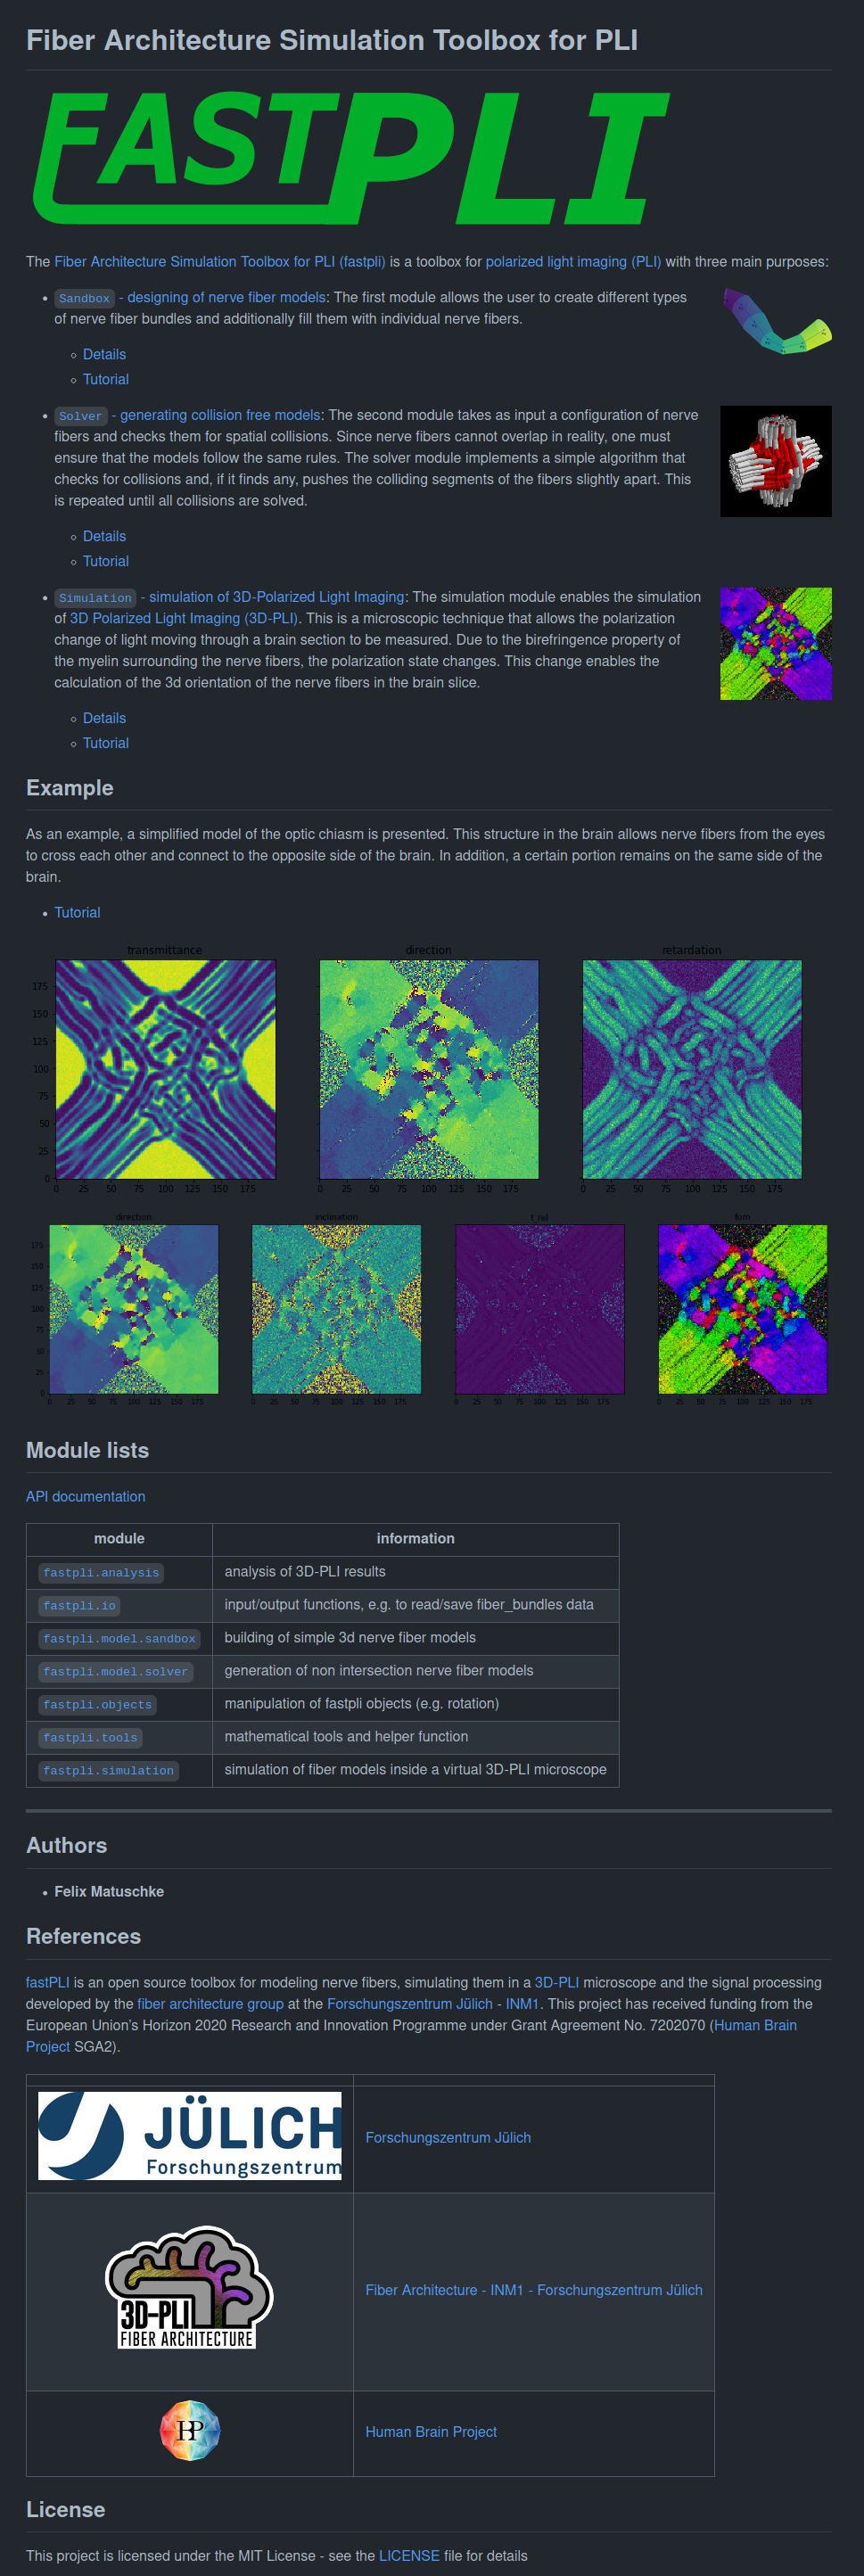
\includegraphics[valign=T,trim=0 1300 0 0, clip]{gfx/fastpli/fastpli_wiki.png} &
 	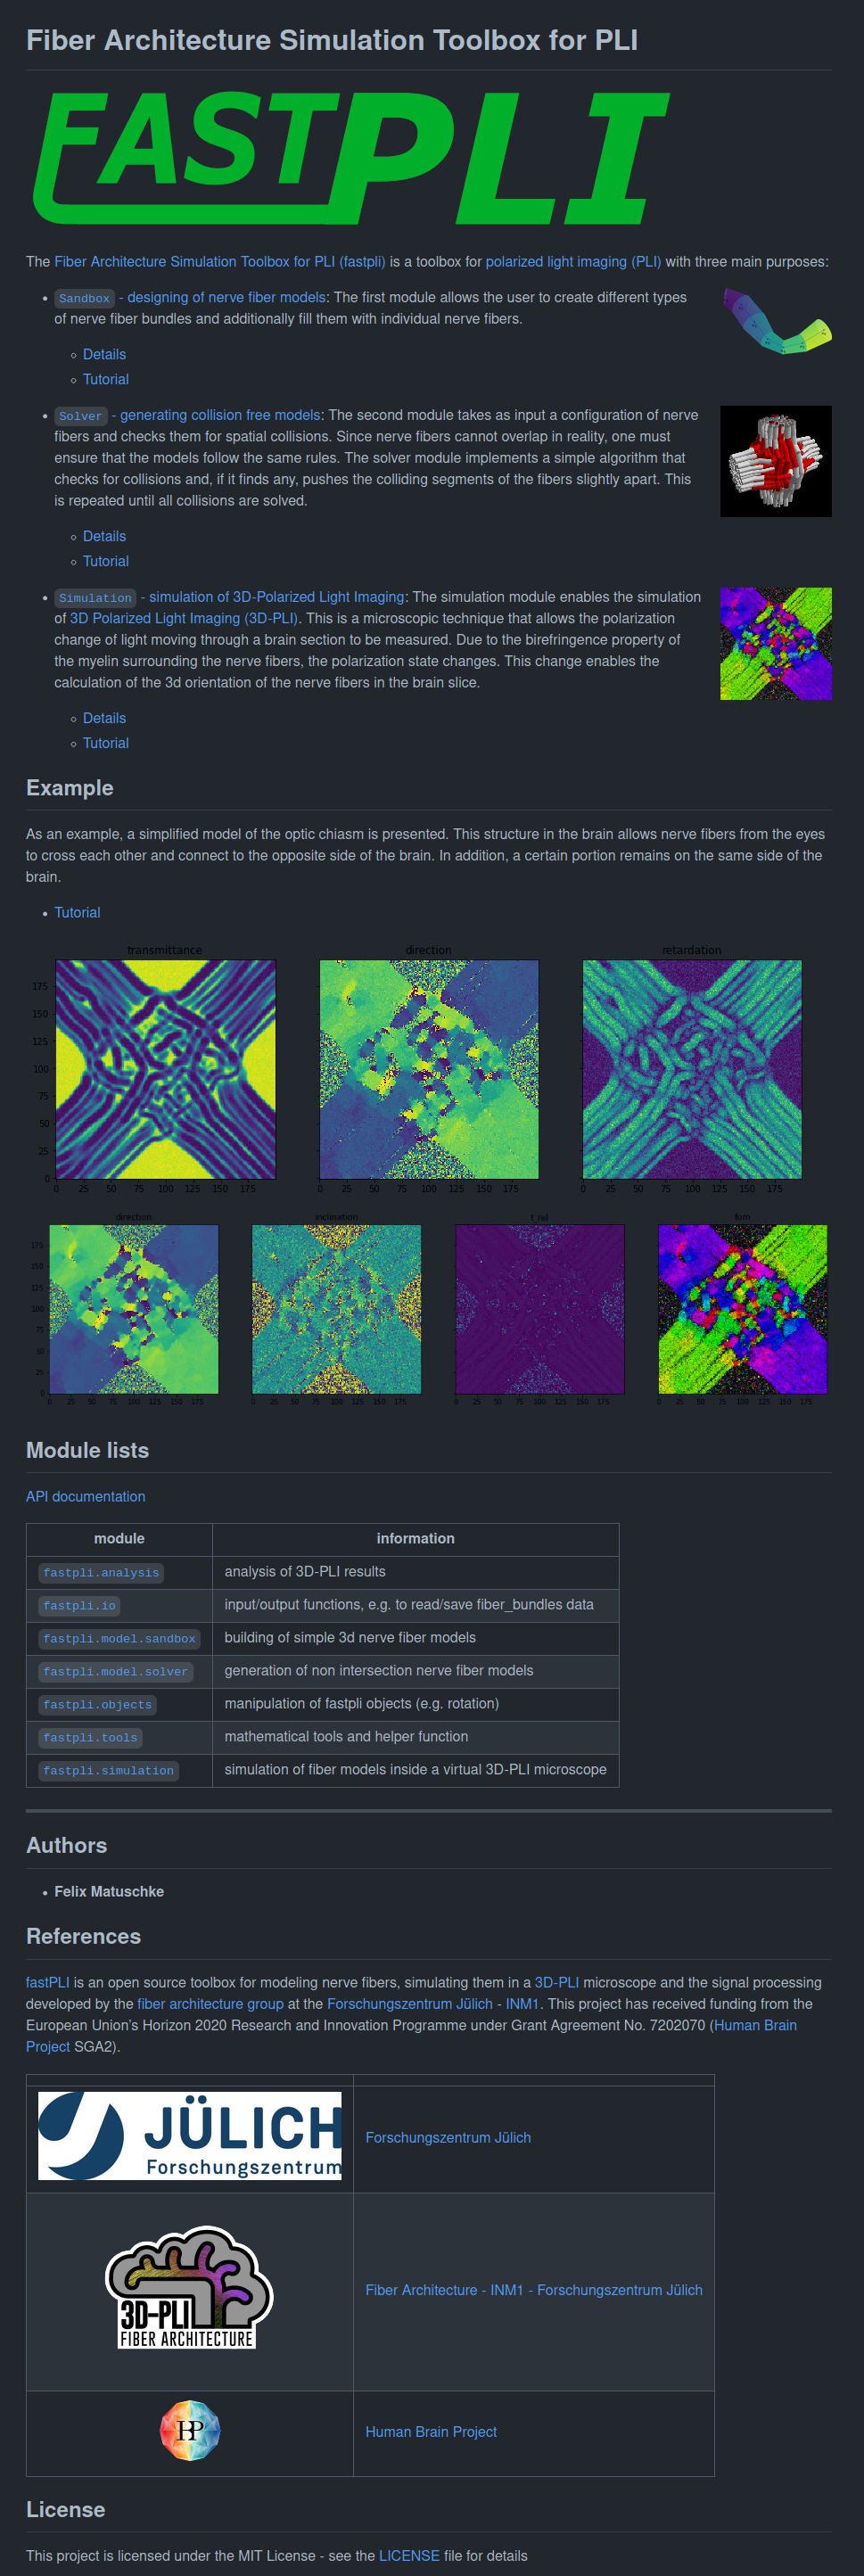
\includegraphics[valign=T,trim=0 0 0 1580, clip]{gfx/fastpli/fastpli_wiki.png} \\
    \end{tabular}
    }}
	\caption{Documentation wiki page of the Github repository \url{https://github.com/3d-pli/fastpli/wiki}.}
	\label{fig:fastpli_wiki}
\end{figure}
%
As is common in software development, all methods are provided with docstrings (documentation strings) so that the user understands their function.
These are, for example, automatically displayed by modern editors during programming to provide assistance.
These docstrings are also used for an automatic release of a \ac{API} documentation.
\footnote{\url{https://3d-pli.github.io/fastpli/}}
In addition to the API, there is a wiki page (see \cref{fig:fastpli_wiki}) that describes the main features, which is an essential part of the review process for release in \ac{JOSS} \cite{Matuschke2021}. 
\footnote{review openly accessible at \url{https://github.com/openjournals/joss-reviews/issues/3042}}
The wiki page is structured like a guide that walks through the aspects of designing nerve fiber models, applying the collision solution algorithm, visualizing nerve fibers, a simple tutorial on \ac{3D-PLI}, and finally applying the models in simulation.
Both executable \python{} scripts and Jupyter notebooks are provided as tutorials to get you started quickly.
For the linking of the individual processes, i.e. generation, simulation and analysis, an example is given of the optic chiasm, the nerve fiber transition of the light pathway from the eyes to the occipital lobe.
%
%
%
\subsection{Dependencies}
%
\paragraph{Python:}
\begin{description}
\item[numpy:] Base N-dimensional array package \cite{2019arXiv190710121V}\\
\url{https://numpy.org/}
\item[scipy:] Fundamental library for scientific computing \cite{2019arXiv190710121V}\\
\url{https://www.scipy.org/}
\item[numba:] Acceleration of Python Functions \cite{Lam2015}\\
\url{https://numba.pydata.org/}
\item[mpi4py:] MPI for Python \cite{Dalcn2005, Dalcn2008, Dalcin2011}\\
\url{https://bitbucket.org/mpi4py/mpi4py/src/master/}
\item[h5py:] HDF5 for Python \cite{collette_python_hdf5_2014, hdf5}\\
\url{https://www.h5py.org/}
\end{description}
%
\paragraph{C++:}
\begin{description}
\item[MPI:] Message Passing Interface \cite{message2015mpi}\\
\url{https://www.mpi-forum.org/}
\item[OpenMP:] Open Multi-Processing, API for multi-platform shared memory multiprocessing programming \cite{dagum1998openmp}\\
\url{https://www.openmp.org/}
\item[OpenGL:] Open Graphics Library \cite{khronos}\\
\url{www.opengl.org}
\item[Pybind11:] Seamless operability between C++11 and Python \cite{pybind11}\\ \url{https://github.com/pybind/pybind11}
\end{description}
%
%
At this point, only Linux builds are supported.
However, for current Windows versions, the \ac{WSL} provides a fully functional Linux kernel within Windows.
This makes it possible to run the same software as on native Linux distributions.
Current macOS versions are not supported, but due to the minimalistic style of the \ac{fastPLI} package, the required changes should be feasible with minimal modifications.
%
%
%
\subsection{Installation}
%
The installation instructions are scripted in a \code{Makefile}.
It first starts a \name{CMake} routine which searches for all the required libraries and programs.
Then the \cpp{} code is compiled and the resulting \name{shared object libraries} are stored in the \python{} routines.
Finally, the provided code \code{setup.py} allows the user to install the compiled package in his environment.
%
\begin{lstfloat}[!ht]
\lstset{style=common}
\begin{lstlisting}
make fastpli
pip3 install .
\end{lstlisting}
\end{lstfloat}
%
%
%
\subsection{Tests, Verification \& Issues}
%
To provide a fully tested software, each module with its main methods is automatically tested with a \name{Github action} after each \name{git push}.
\footnote{github actions are commonly used to automatically build, test, and deploy the software and documentation}.
\footnote{uploud of the current \textit{software stage}.}
This action runs the two latest Ubuntu Long Term Support versions (currently 18.04 LTS and 20.04 LTS) and the most commonly used Python3 versions (currently 3.6 and 3.8) to provide a wide range of supported common versions.
In addition, the \name{Github actions} run all test scripts, check tutorial files, check code format and linting for consistency, and publish the latest documentation after a sucessfull tested release.
\par
%
Github allows to track \name{Issues}.
This feature is originally used to document software bugs.
However, it is also used to discuss ideas, new features, and so on.
As part of the open source release, it was also used communicate with the reviewer.
\footnote{\url{https://github.com/openjournals/joss-reviews/issues/3042}}
This allows to always track back the development process and code changes in addition with the git \name{commits}.
%
% 
% 
\section{Modules}
%
A \python{} \name{package} consists of \name{modules} which contain the definitions of functions, classes and so on.
In the following the different modules are listed alphabetically.
%
%
%
\subsection{\Code{fastpli.analysis}}
%
This module contains all functionalities to analyze the \ac{3D-PLI} simulations analogous to the routine measurements.
This includes the analysis of the signal to the three image modalities transmission, direction and retardation.
Furthermore, it provides the tilting analysis \ac{ROFL} \cite{Schmitz2018}.
In addition, further helper functions exist that provide methods to convert the direction and tilt results into a \ac{FOM}.
\par
% 
For the analysis of fiber models, the module providing a few simple helper functions.
This for example allow the user to generate a histogramm of the orientations of the fiber segments like the ones shown in this thesis.
%
% 
% 
\subsection{\Code{fastpli.io}}
%
This method provides the read and write routines that allow the user to load and save fiber models (\ie{} \code{fiber\_bundles}) to or from disk.
There are two formats available.
The first is a simple text file with the extension \code{.dat} (see \cref{alg:dat-file}).
Here, each $(x,y,z,r)$ tuple of a fiber point is stored as a single line in the file.
Two fibers are separated by one blank line, while two fiber bundles are separated by two blank lines.
This data format is provided to allow a very simple format for manipulating, exchanging and \eg{} reading the files into other programs.
\par
%
\begin{lstfloat}[!ht]
\lstset{style=common,morecomment=[l][\color{syntax_green}]{##},}
\begin{lstlisting}
-6.55 -18.93 -64.98 3.75 # x y z r
-5.73 -14.89 -63.37 3.4
-4.42 -13.66 -58.95 3.05
                         # empty line indicates new fiber
-1.96 -10.07 -52.5 2.92
-1.03 -9.4 -48.62 2.93

                         # two empty lines indicates new fiber bundle
3.4 -4.02 -44.76 3.11
6.22 -1.04 -42.45 3.26
\end{lstlisting}
\caption{Exemplary \name{.dat} file format. Comments are not allowed.}\label{alg:dat-file}
\end{lstfloat}
%
The second format uses \ac{HDF5} \cite{hdf5} which uses a binary data format.
\ac{HDF5} allows the data to be stored as \name{datasets} in \name{groups}.
This is analogous to a file in an operating system being stored in folders.
The \ac{HDF5}-\name{groups} are used to store the \code{fiber} in \code{fiber\_bundle} and \code{fiber\_bundles}.
The $(x,y,z,r)$ information of each fiber is then stored as a 2d-array (see \cref{alg:hdf5}).
%
\begin{lstfloat}[!ht]
\lstset{style=common,morecomment=[l][\color{syntax_green}]{##},}
\begin{lstlisting}
GROUP "/" { # fiber_bundles path
  GROUP "0" { # id of fiber_bundle
      DATASET "0" { # id of fiber
         DATATYPE  H5T_IEEE_F64LE
         DATASPACE  SIMPLE { ( 3, 4 ) / ( 3, 4 ) }
         DATA {
         (0,0): -6.55, -18.93, -64.98, 3.75,
         (1,0): -5.73, -14.89, -63.37, 3.4,
         (2,0): -4.42, -13.66, -58.95, 3.05,
         }
      }
      DATASET "1" { # id of fiber
         DATATYPE  H5T_IEEE_F64LE
         DATASPACE  SIMPLE { ( 2, 4 ) / ( 2, 4 ) }
         DATA {
         (0,0): -1.96, -10.07, -52.5, 2.92,
         (1,0): -1.03, -9.4, -48.62, 2.93,
         }
      }
  }
  GROUP "1" { # id of fiber_bundle
      DATASET "0" { # id of fiber
         DATATYPE  H5T_IEEE_F64LE
         DATASPACE  SIMPLE { ( 2, 4 ) / ( 2, 4 ) }
         DATA {
         (0,0): 3.4, -4.02, -44.76, 3.11,
         (1,0): 6.22, -1.04, -42.45, 3.26,
         }
      }
  }
}
\end{lstlisting}
\caption{Example structure of the fiber format in \ac{HDF5}. This output is generated with the official \code{h5dump} tool.}
\label{alg:hdf5}
\end{lstfloat}
%
%
%
\subsection{\Code{fastpli.model.sandbox}}
%
This module provides all the functions described in \cref{sec:sandbox}.
The module is divided into two submodules: \code{fastpli.sandbox.build} and \code{fastpli.sandbox.seeds}.
\code{fastpli.sandbox.seeds} contains all the methods for populating a 2d-plane, as described in \cref{sec:seeds}.
To populate the fiber from the seeds, the \code{sandbox.build} module provides the methods.
This includes all the described functions from \cref{sec:fillBundle}.
%
%
%
\subsection{\Code{fastpli.model.solver}}
%
The module \code{fastpli.model.solver} contains the compiled solver algorithm, which is explained in detail in \crefrange{sec:Solver}{sec:modelOpt}.
Additionally, the solver algorithm is wrapped in the \code{fastpli.model.solver.Solver} class.
This wrapper class provides a higher level of abstraction (see \cref{sec:fastpliIntro}).
It contains all necessary variables as attributes and therefore provides read/write access via class properties, \eg{} \code{Solver.obj\_mean\_length}.
Each write method checks the input for user errors and returns an appropriate warning or error message.
This class also includes a \code{Solver.get\_dict()} method that returns a \python{} dictionary containing all variables and their values for reproducibility.
It is also possible to store the state of the class with the current state of the \code{fiber\_bundles} as an \ac{HDF5} object.
Finally, this class also provides the possibility to use a simple visualization (see \cref{sec:visualization}) of the solution process.
%
%
%
\subsection{\Code{fastpli.objects}}
%
This module provides a wrapper class for \code{fastpli.objects.fibers} and \code{fastpli.objects.layers}.
Essentially, \code{layers} are a \code{list} of \code{layers}, which in turn are a \code{tuple} of the four attributes \code{absorption}, \code{birefringence}, \code{model}, and \code{scale} (see \cref{sec:dv_generator}).
This wrapper class contains attributes that allow the user to access these values by name, rather than by index \code{tuple} \code{[i]}.
This is helpful to reduce user errors.
\par
% 
The same is true for \code{fastpli.objects.fibers} which contain \code{fastpli.objects.FiberBundles}, \code{fastpli.objects.FiberBundle} and \code{fastpli.objects.Fiber} classes with the same purpose.
\code{FiberBundles} are a \code{list} of \code{FiberBundle} which are a list of \code{Fiber}.
The data of a fiber is stored in a \code{numpy.ndarray} which stores the values contiguously in memory.
Manipulation methods are provided for each class, allowing the user to \code{translate}, \code{rotate}, \code{scale}, and \code{cut} the model.
The latter helps especially in the solution process to reduce the number of objects if only a certain volume is to be generated, since the solution process pushes the fiber objects apart and thus the volume would be increased.
%
%
%
\subsection{\Code{fastpli.simulation}}
% 
Like the \code{fastpli.model.solver.Solver} class, this method provides a wrapper for simulation called \code{fastpli.simulation.Simpli}, which is based on the original algorithm \cite{Dohmen2015,Lucksch2016}.
It contains the two algorithms \code{generator} and \code{simulation} described in \cref{sec:dv_generator,sec:simulation}.
These two algorithms operate separately, but since they share a number of parameters, they coexist within the class.
As in the \code{fastpli.model.solver.Solver} class, all necessary attributes are available and checked for input errors.
Since analysis is usually always performed on the resulting simulations, they are also available in this class and are performed with the same defined parameters as in the simulation.
Methods for saving the variables as \code{dict} or \ac{HDF5} files are also available.
\par
% 
As in the experiment, the simulations can run with the same routine.
This means that many parameters and the simulation pipeline usually do not change.
For this purpose there are \code{pipeline} methods (see \cref{alg:Pipeline}) which provide a high level of abstraction.
Here, all data is automatically analyzed and stored.
%
\begin{lstfloat}[!tb]
\centering
\scalebox{0.75}{
\begin{minipage}{\the\textwidth}
\lstinputlisting[style=python]{code/pipeline.py.tex}
\end{minipage}}
\caption{Simulation pipeline \code{simpli.run\_pipeline()}.}
\label{alg:Pipeline}
\end{lstfloat}
%
%
\subsection{\Code{fastpli.tools}}
% 
The last module contains a set of helper functions.
They provide access to the current version as well as to the git hash so that all calculations can be reproduced.
For fiber modeling, rotation matrices are provided to allow the use of linear algebra.
%
\cleardoublepage
\part{Results}
% \acbarrier
\parttoc
\setcounter{chapter}{6}
\chapter{Dense \acs{WM} modelling analysis}
\label{cha:model_analysis}
% 
\todo{veroffentlichung in intro}
% 
\itodo{reproduzieren von modellen}
% 
\section{Introduction}
% 
After describing the functionality of the \pymodule{fastpli.model}, the next task is to use these methods not only to create realistic dense \ac{WM} models, but to keep them as simple as possible due to the complexity of the tissue.
This is due to the fact that \ac{WM} contains individual nerve fibers that typically have a size in the order of about $\SI{1}{\micro\meter}$.
Therefore, in a \SI{60}{\micro\meter} voxel of a \ac{LAP} measured \ac{3D-PLI} can be image within the \ac{WM} several thousand individual nerve fibers are already present.
Considering that each nerve fiber has a unique trajectory through this volume, this means that theoretically an absurd variety of possible configurations exists.
However, due to the nature of the \ac{3D-PLI} structure, previous studies have shown that the result of the signal depends on much less degrees of freedom than each individual nerve fiber has.
\\[\baselineskip]
% 
Therefore, this work, being the first study of its kind, focuses mainly on two randomly interwoven fiber populations for \ac{3D-PLI} simulations.
Another focus is the generation of such models, whereby the computational time effort shall be kept as low as possible.
The analysis refers to the setting of the parameters for the model generation and their influence on the resulting collision-free configurations.
% 
% 
\section{Brain tissue model}
% 
To create universal reusable \ac{WM} tissue models, a practical approach is to reduce the number of parameters to a minimum.
The approach chosen here is to build cubic volumes of up to two fiber populations with individual characterization.
The most important parameter for \ac{3D-PLI} is orientation.
% 
\subsection{single fiber bundle population}
% 
A single fiber bundle population can have any orientation $O(\varphi,\alpha)$ in 3d space.
However, since $O(\varphi,\alpha) = O(\varphi+\pi,-\alpha)$ only the orientations of a hemisphere are required.
Furthermore, the experimental setup does not allow a difference between a fiber bundle population with $\varphi = \varphi_0$ and $\varphi = \varphi_1$ when the initial optical elements are rotated by $\varphi_1-\varphi_0$, unless one considers the effect of the physical expansion of the camera pixels, which is neglected here.
Therefore it is not necessary to create a single fiber population with a direction other than $\varphi = \SI{0}{\degree}$.
However, the inclination must be sampled in the range of $[0,90]\si{\degree}$.
Since the fiber bundle populations can easily be rotate from $\varphi=\SI{0}{\degree}, \alpha=\SI{0}{\degree}$ to $\varphi=\varphi_{\text{target}}, \alpha=\alpha_{\text{target}}$, it is not necessary to create individual fiber bundle configurations.
\\
%
\paragraph{fiber distribution}
To initialize the trajectories the previous introduced method for building a cubic volume is be used (see \cref{sec:cubeModelBuilding}) along the fiber bundle population orientation $F = O(\varphi, \alpha)$.
The seeding along the fiber bundle population will be randomly set with:
\begin{align}
p = \mathrm{sample}\left(\mathrm{Uniform}(\sqrt{3}*\mathit{cube\_size})\right)
\end{align}
Each fiber will have an individual radii, sampled from a \name{log normal} distribution $\mathrm{LogNorm(
\mu,\sigma)}$ (see \cref{fig:logNormal}).
Its probability desity function looks like this:
\begin{align}
\mathrm{LogNorm}(x,\mu,\sigma)=\frac{1}{\sigma x \sqrt{2\pi}}\exp\left(-\frac{(\ln(x)-\mu)^2}{2 \sigma^2}\right)
\end{align}
% 
Its property allows to multiply by a logarithmic mean value $\fiberRadiusMu=0$ to sample values which are not allowed to have negative values like a length and keeping the desired mean value $\fiberRadiusMean$:
\begin{align}
\fiberRadius = \fiberRadiusMean \cdot \mathrm{sample}\left(\mathrm{LogNorm}(\mu=0,\sigma=0.1)\right)
\end{align}
% 
\begin{figure}[!t]
\centering
\tikzset{external/export=false}
\begin{tikzpicture}[scale=1, trim axis left, trim axis right]
\begin{axis}[height=0.46\textwidth, width=0.75\textwidth,enlargelimits=false, xlabel={$x$}, ylabel={$f(x,\mu,\sigma)$}, title=${f(x,\mu,\sigma)=\frac{1}{\sigma x \sqrt{2\pi}}\exp\left(-\frac{(\ln(x)-\mu)^2}{2 \sigma^2}\right)}$,
legend style={at={(1,1)},anchor=north east},
legend cell align={left},
]
\pgfmathsetmacro{\muValue}{0}
\pgfmathsetmacro{\sigmaValue}{0.05}
\addplot[BLUE,thick,domain=0.6:1.4, samples=2*42, smooth]{1/(\sigmaValue*x*sqrt(2*pi))*exp(-(ln(x)-\muValue)^2/(2*\sigmaValue^2))}; \addlegendentry{$\mu=0.0,\sigma=0.05$}
\pgfmathsetmacro{\muValue}{0}
\pgfmathsetmacro{\sigmaValue}{0.1}
\addplot[GREEN,thick,domain=0.6:1.4, samples=2*42, smooth]{1/(\sigmaValue*x*sqrt(2*pi))*exp(-(ln(x)-\muValue)^2/(2*\sigmaValue^2))}; \addlegendentry{$\mu=0.0,\sigma=0.1$}
\end{axis}
\end{tikzpicture}
\caption[]{\itodo{check values in literatur} Probability density function of a multiplicative \name{log normal} distribution.}
\label{fig:logNormal}
\end{figure}
% 
\paragraph{fiber segmentation}
%
To split the current straight fibers into segments for the next step, the \pymodule{fastpli.model.solver} process is used.
Each fiber is split into a mean length of $\segLength$.
%
\paragraph{fiber deformation}
After the initial seeding process, and after applying the model segment length, each \name{sphere} of a fiber will be randomly changed.
The point will be randomly displaced by a normal distribution and the radii with the log normal distribution $(\mu=0,\sigma=0.05)$.
% 
\begin{align}
\begin{split}
p &= p + \mathrm{sample}\left(\mathrm{Gaus}(\mu=0,\sigma=0.05 \cdot \fiberRadiusMean)\right)\\
r &= \fiberRadius \cdot \mathrm{sample}\left(\mathrm{LogNorm}(\mu=0,\sigma=0.05)\right)
\end{split}
\end{align}
% 
This will produce a pseudo random initial configuration for the collision solving process.
% 
\subsection{dual fiber bundle populations}
The same mathematical properties as above are true for any fiber population $F$ inside a superposition.
This means, that only a differential angle between the two orientations, so called crossing angle $\modelOmega$, is needed as well as a proportion change between both populations $\modelPsi{} = N(F_0)/N(F_G)$.
% in:
% \begin{align}
%     F_G = [\modelPsi \cdot F_0] \circ [(1-\modelPsi) \cdot F_1]
% \end{align}
% 
Since the direction of the first fiber bundle population can be again neglected, only the direction and inclination of the second fiber population relative to the first is important. Therefore it was decided to build models with \modelOmega{} from ${0,10,...,90}$ and afterwords rotating the fiber orientations around the x axis (\cref{fig:twomodelpop})
% 
% \paragraph{rest}
% % 
% As described in \cref{chap5:ShapeControl} the choice of shape parameters \segLength and \segRadius are quite important. For a realistic fiber radius distribution of around \SI{0.5}{\micro\meter} the time for a \SI{60}{\micro\meter} usable cube (\SI{105}{\micro\meter} sphere) varies from several hours up to \SI{24}{\hour}.
% 
\begin{figure}[p]
\centering
\def\tikzwidth{0.42*\textwidth}
\subcaptionbox{\label{fig:modelrotcube}A spherical volume with diameter $d$ is used as boundary, so that a cube of side length $1/1.5 \cdot d$ can be cut in any orientation inside the sphere.}
[.49\textwidth]{\inputtikz{gfx/model/sphere_cube}}\hfill
\subcaptionbox{\label{fig:modelinit}Initial orientation for two fiber populations $F_0$ and $F_1$. The angle between both populations is $\Omega$. The remaining degree of freedom are taken into account by rotating the whole volume (see \cref{fig:modelrotcube})}
[.49\textwidth]{\inputtikz{gfx/model/sphere_models}}
\\
% 
\subcaptionbox{fixed first fiber population; half rotation of second fiber population}
[.49\textwidth]{\inputtikz{gfx/model/sphere_models_a}}\hfill
\subcaptionbox{\label{subfig:Test1}increasing inclination for first fiber population}
[.49\textwidth]{\inputtikz{gfx/model/sphere_models_b}}
\\
% 
\def\tikzwidth{0.35*\textwidth}
\subcaptionbox{\label{subfig:sphere:hista1} hist a}
[.49\textwidth]{\inputtikz{gfx/model/sphere_hist_a}}\hfill
\subcaptionbox{\label{subfig:sphere:histb} hist b, with applied symmetries.}
[.49\textwidth]{\inputtikz{gfx/model/sphere_hist_b}}
\caption{two population model library \itodo{centering} \itodo{e und f fertig machen}}
\label{fig:twomodelpop}
\end{figure}
% 
% \begin{figure}[t!]
% \centering
% \includegraphics[width=0.5\textwidth]{dev/gfx/htm_levels.png}
% \caption{htm}
% \label{fig:htm}
% \end{figure}
%  
% 
\subsection{Algorithmic setup}\label{sec:modelSetup}
% 
To find a usable library of two fiber populations researched main attributes are listed in \cref{tab:cube2pop} \cref{tab:cube2popSoftware} contains the parameters of the additional \pymodule{fastpli.model.solver} algorithm. All \dummy{} will be repeated five times.
\itodo{AT THE END OF EACH STEP THE VOLUME TO SOLVE IS ALWAYS CUTTED TO 105.}
% 
\begin{table}[!b]
\sisetup{parse-numbers=false,open-bracket={\{}, close-bracket={\}}, list-final-separator={,},list-pair-separator={,}}%
\centering
\pgfplotstabletypeset[%
    thesisTableStyle,
    column type=lcl,
    columns/name/.style={string type},
    columns/variable/.style={string type},
    columns/values/.style={string type},
    every head row/.style={before row=\toprule,after row=\midrule},
    every last row/.style={after row=\bottomrule},
    col sep=&,
    row sep=\\,
    % string type,
]
{name & variable & values\\
mean fiber radius & $\textcolor{violet}{\fiberRadiusMean}$ & $\SIlist{0.5;1;2;5;10}{\micro\meter}$\\
mean segment length factor & $\textcolor{violet}{\segLengthFactor}$ & $\numlist{1;2;4;8}$\\
min segment bending radii factor & $\textcolor{violet}{\segRadiusFactor}$ & $\numlist{1;2;4;8}$\\
fiber bundle distribution value & $\textcolor{violet}{\modelPsi}$ & $\numlist{0.1;0.2;...;1.0}$ \\
fiber bundle crossing angle & $\textcolor{violet}{\modelOmega}$ & $\SIlist{0;10;...;90}{\degree}$\\
}
\caption{parameter\_statistic setup and \textcolor{violet}{variables}.}
\label{tab:cube2pop}
\end{table}
% 
\begin{table}[!b]
\centering
\sisetup{open-bracket={\{}, close-bracket={\}}, list-final-separator={,},list-pair-separator={,}}%
\pgfplotstabletypeset[%
    thesisTableStyle,
    column type=l,
    columns/variable/.style={string type},
    columns/value/.style={string type},
    every head row/.style={before row=\toprule,after row=\midrule},
    every last row/.style={after row=\bottomrule},
    col sep=&,
    row sep=\\,
]
{variable & value\\
pre model diameter & $d = \SI{120}{\micro\meter}$\\
mean fiber radius & $\textcolor{violet}{\fiberRadiusMean} = \SIlist{0.5;1;2;5;10}{\micro\meter}$\\
fiber radius distribution & $\fiberRadiusSig = \SI{0.1}{}$, $\fiberRadiusMu = \SI{0}{\micro\meter}$\\
seed.distance & $2 \cdot \textcolor{violet}{\fiberRadiusMean}$\\
seed.size & $2 \cdot \mathit{volume}$\\
bundle distribution & $\textcolor{violet}{\modelPsi}$\\
bundle crossing & $\textcolor{violet}{\modelOmega}$\\
solver.obj\_mean\_length & $\textcolor{violet}{\fiberRadiusMean} \cdot \textcolor{violet}{\segLengthFactor}$\\
solver.obj\_min\_radius & $\textcolor{violet}{\fiberRadiusMean} \cdot \textcolor{violet}{\segRadiusFactor}$\\
solver.max\_steps & $\SI{100000}{}$\\
max runtime & $\SI{24}{\hour}$\\
}
\caption{parameter\_statistic setup and \textcolor{violet}{variables}.}
\label{tab:cube2popSoftware}
\end{table}
\todo{show radius distribution}
% 
\subsection{Results}
% 
\paragraph{Volume fraction}
% 
\begin{figure}[p]
\centering
\includegraphics[width=\textwidth, page=1]{dev/gfx/2/parameter_statistic_box_plot_volume.pdf}
\caption[Model characteristics]{Model characteristic for $\fiberRadius = \SI{1}{\micro\meter}$ different parameters. \itodo{\segLengthFactor{} and \segRadiusFactor{}}}
\label{fig:psbp1}
\end{figure}
% 
\cref{fig:psbp1} show the resulting volume fraction $V/V_0$ for the parameter series.
Non crossing angles $||$ achive clearly a higher fraction of $V/V_0 > 0.75$ than their counter crossing parts $cross$.
Their value also is for fibers with radii $\fiberRadius <= \SI{5}{\micro\meter}$ very stable for all five repeats.
Further the volume fraction is stable for changes along the parameter $\segLengthFactor$ and $\segRadiusFactor$. 
Only the fibers with a radius of $\fiberRadius = \SI{10}{\micro\meter}$ achive smaler fractions and slighty unstable results with Values around \dummy{}.
\\
The crossing \dummy{} show a clear decrease volume fraction along a increase of the $\segLengthFactor$ as well as a slightly decrease with increasing $\segRadiusFactor$ for all fiber radii.
The decrease with the change of $\segLengthFactor$ stabilises around $\segLengthFactor = \num{8}$.
For smaller fiber radii the repeating process is more stable as for larger radii.
\\
Overall the volume fraction stays above 0.75 for parallel and fr > 2.
For crossing fibers in this range the value stays above around 0.5.
% 
\paragraph{Time development}
% 
\begin{figure}[p]
\centering
\includegraphics[width=\textwidth, page=2]{dev/gfx/2/parameter_statistic_time_evolve.pdf}
\caption[Time development parallel]{Time development of the model generation process of parallel fiber populations. non crossing\itodo{\segLengthFactor and \segRadiusFactor}\itodo{title}\itodo{units}}
\label{fig:timeDevelopmentNone}
\end{figure}
% 
\begin{figure}[p]
\centering
\includegraphics[width=\textwidth, page=1]{dev/gfx/2/parameter_statistic_time_evolve.pdf}
\caption[Time development parallel]{Time development of the model generation process of parallel fiber populations. crossing \itodo{\segLengthFactor and \segRadiusFactor}\itodo{title}\itodo{units}\itodo{restlichen parameter anhang}}
\label{fig:timeDevelopmentCross}
\end{figure}
% 
The change in time of the properties are shown in \cref{fig:timeDevelopmentNone,fig:timeDevelopmentCross}.
Looking at only the non crossing models \cref{fig:timeDevelopmentNone} shows a linear correlation between the number of steps and the time.
All models have a step size smaller than the maximal step size, therefore are completely solved and the last plotted value corresponds to the total time consumption for each parameter set.
The change of $\segLengthFactor$ has no significant influence.
An increase in $\segRadiusFactor$ on the other side clearly increases the log(time) consumption up to several order of magnitudes.
\\
% 
Looking at the number of colliding objects they correlate with the time (non log!). 
Again a change in $\segLengthFactor$ has no significant effect and an increase in $\segRadiusFactor$ increases the time consumption up to several order of magnitudes.
\\
% 
The overlap fraction coresponts to the overlapping distance/distance in total of all remaining colliding objects.
Its value at the start is non higher of \SI{8}{\percent} \dummy{}.
The values are decreasing similar to the number of colliding objects, however not as fast.
As before, a change in $\segLengthFactor$ has no significant effect and an increase in $\segRadiusFactor$ increases the time consumption up to several order of magnitudes.
% 
The comparison to crossing models in \cref{fig:timeDevelopmentCross} shows for all parameters a very similar behavior.
The development of the number of steps is exactly as for the linear case, expect that the number of steps are higher.
fl=\dummy{} and fl= \dummy{} reach the maximal number of steps, but not the maximal time value.
\todo{human time values in plot}.
The number of objects and overlapping fraction value show a splitting behavior for a change in $\segLengthFactor$.
For smaller values the time consumption is significantly (log!) smaller.
larger values show a stagnant behavior for the parameters, however already for small values (log!).
A change in $\segRadiusFactor$  increases the time consumption up to several order of magnitudes as in the linear bundle case.
% 
% 
% 
\subsection{Discussion}
% 
The goal is to choice a set of parameters, which allow a) fast, b) collision free and c) a high volume fraction for densely fibers.
In the case of parallel fibers, the solving process is always faster than for crossing bundles.
Even thow that the number of colliding objects is more or less \dummy{} the same \comment{(ein plot?)} the needed volume to have enough space to not collide with each other is larger \dummy{}.
Therefore the distance the fiber segments have to travel is higher und the number of steps to achive this increases as well.
\\
% 
The behavior in change of the length factor \segLengthFactor{} is clearly a time advantage, since also the number ob objects is smaller.
However a larger \segLengthFactor{} results for crossing fibers as to be expected in a smaller volume fraction.
For parallel fiber is is reasonable that the volume fraction das not change, since the direction of movement for all fiber segments is radial symmetric along their main orientation axis.
Up to a fiber radii of \SI{2}{\micro\meter} the repeating measurements are stable.
Above it the resulting orientations starts to divers.
This has to to with that the volume has a fixed size of \SI{60}{\micro\meter}.
This means the number of segments is quite small, individual and the model is therefore diverge.
\\
The fiber semgent bending radii factor \segRadiusFactor{} yield to less diverse results.
Since it restrict the bending radii, it is expected, and visible in the results, that the volume fraction is very influenced, since the volume can't be optimal filled anymore.
Again changes parallel fiber orientation are almost not visible, for all analysed values.
Crossing fibers however are as expected influenced.
This is especial visible in the number of colliding objects, where the \segRadiusFactor{} splits the data into individual branches over time.
Since smaller values of \segRadiusFactor{} allow more curved geometries, this is as expected.
However this can lead to \say{strange looking} results and has to be set with an anatomical perspective. \todo{images}
\\[\baselineskip]
% 
Overall the choice of the parameters can be narrowed.
The main decision come from the crossing results.
Since most basic parameter is the length length factor \segLengthFactor{}.
Looking at the volume fraction results it should be as small as possible.
However since the difference between $\segLengthFactor=\SI{1}{}$ and $\segLengthFactor=\SI{2}{}$ is small, and a big leap is visible for $\segLengthFactor=\SI{4}{}$ one can use $\segLengthFactor=\SI{2}{}$.
The only reason to increase this value further would be a reduction in computational time.
\\
% 
The fiber radii should be as realistic to real \acs{WM} brain tissue as possible.
However to reduce the computational time further, a reduction to $r = \SI{1}{\micro\meter}$ is feasible.
It is still in the same order of magnitude to the real values (\SI{0.5}{\micro\meter}).
The \ac{3D-PLI} simulation results will show more effective metric to further restrict these parameters.
% 
The choice of the fiber banding factor is as already mentioned, more a anatomical restriction.
However it can be resend, that it has no benefit to reduce its value more then 1 or fibers can (with a small fiber segment length) move perfectly around another fiber, like horseshoe shaped.
To work against this, but not to further restrict the model geometry a value of 2 is chosen.
Therefore $\segLengthFactor = \SI{2}{}, \segLengthFactor=\SI{2}{}$ and $\fiberRadius=\SI{1}{\micro\meter}$.
\\
% 
A last remark.
An additional property to reduce the computational time is to not completely solve the model. 
Looking at the overlap fraction of the remaining overlapping segments, a value of $<\SI{1}{\percent}$ can be feasible.
This this an additional order of magnitude can be potential saved.
However, the effect inside the simulation has to be studied.
% 
\section{CPU Acceleration}
% 
\begin{figure}[!t]
\centering
\includegraphics[]{dev/gfx/4/model_solver_cubes.pdf}
\caption[speedup]{\itodo{cores, not threads} \itodo{farben?}}
\label{fig:solverSpeedup}
\end{figure}
% 
\itodo{Welche Parameter ...}
% 
As described in \dummy{} \openmp{} is used for acceleration.
This means no usage of multiple computer nodes is currently available.
\cref{fig:solverSpeedup} shows a speedup up to eight cores.
A number of two cores gives a good speedup of around $1.8$, three cores around $2.5$ and four cores around $3$.
A further incresse of core numbers does not benefit the computational time much.
This has most likely to do with the fact, that the data has to transvered between all the cores and this takes quite some time.
Even if the algorithm is especially optimized to reduce the amount of data to be copied, the paralysed instructions are often very short (\eg{} move positions), with the exception of the distance calculation.
Since all data is linear in memory, the cpu can use the full potential of the prefetcher and calculate very fast.
\\[\baselineskip]
% 
The results show, that especially to increase the volume size, other algorithms are needed. 
Here the \ac{GPU} seems to be the hardware of choice.
% 
\section{Building models for simulation}
% 
With the upper chosen model parameters the final models can be build.
To be able to study the effect of the fiber radii on the simulation, all radii are generated.
In this section the resulting orientation inside the volume, \ie{} the orientation of the fiber segments, will be analysed.
The same setup as above (see \cref{sec:modelSetup}) is chosen with fix $\segLengthFactor=\SI{2}{}$ and $\segRadiusFactor = \SI{2}{}$.
Using the rotational model from above, only fibers with a $\Psi =  0...90$ and $\Omega = 0.1...1.0$ are generated.
% 
\subsection{Results}
% 
\begin{figure}[!t]
\centering
% \resizebox{1.0\textwidth}{!}{
\includegraphics[width=\textwidth, page=1]{dev/rc1/cube_2pop_orientation_hist2d_output_cube_2pop_135_rc1_.pdf}
% }
\caption[Model orientation histograms]{distribution of fiber segment orientation in initial and resulting models for $\fiberRadius = \SI{1}{\micro\meter}$. \itodo{fit ESAG} \ITODO{these are only resulting models!}}
\label{fig:modelOrientation}
\end{figure}
% 
\begin{figure}[p]
\centering
% \resizebox{1.0\textwidth}{!}{
\includegraphics[width=\textwidth, page=1]{dev/rc1/cube_2pop_orientation_hist_output_cube_2pop_135_rc1_.pdf}
% }
\caption[Model orientation histograms]{Maximum normed distribution of fiber segment orientation in initial and resulting models. The left half circle contains the inclination $\alpha$ value, the right half the direction $\varphi$. \itodo{which norm?}}
\label{fig:modelOrientationHist1d}
\end{figure}
% 
The results are visualized in two polar axis plots in \cref{fig:modelOrientationHist1d}. On the right hemisphere the direction histogram is shown.
The left hemisphere shows the inclination distribution.
Both plots are decoupled from each other. \todo{histograms mit line plots?}
Each value is normed to the maximum of that curve so that the shape is visible.
A 3d visualized model is printed in the corner of each parameterset.
% 
The subset of results show that for all radii the fibers rich the same resulting distribution of orientations. 
These distributions are broder than the inital values and are centered around their initial orientations.
The resulting 3d visualized models show all an interwoven structure, where both fiber population orientations are clearly visible. \todo{anhang}
%  
\subsection{Discussion}
% 
\vspace{5pt}
\hrule
\vspace{6pt}
% 

%
\cleardoublepage
\setcounter{chapter}{7}
\chapter{Simulation}
\label{cha:simulation_analysis}
% \minitoc
% 
% 
% 
This chapter contains focuses on the simulation of \ac{3D-PLI}.
The first part focuses on the definition of all necessary parameters.
A part of this is to determined how accurate the simulation has to be, i.e. the voxel size.
Following this, these parameters are used to simulate the previously generated models.
A focus is placed on the accuracy of tilt analyses for different orientations and crossing configurations.
% 
% 
% 
\itodo{reproduzieren von modellen}
% 
% 
% 
\section{Experimental Parameters}\label{sec:sim_choose_parameters}
% 
\subsection{optical resolution}
% 
An optical microscope has a certain resolution. This is often defined in the literature by Abbe diffraction limit. Ernst Abbe found out that the resolution of a light microscope is related to the wavelength of the light $\lambda$:
\begin{align}
d=\frac{ \lambda}{2 n \sin \theta} = \frac{\lambda}{2\mathrm{NA}}
\end{align}
.
$d$ is the minimal resolvable distance, $n$ the refcative index, $\theta$ the angle of a spot light. Further $n \sin \theta$ is better known as the numerical aperture $\mathrm{NA}$.
However, this only sets the maximum resolution. 
Every optical microscope has imaging errors.
The most common are lens aberration, chromatic aberration, ...
All these errors lead to a reduced resolution.
In addition, the sensor that captures the image also plays a role.
For a ccd sensor, this is the configuration of the pixels and their size.
% 
Mathematically, a resolution reduction of an image is modeled by a convolution with a Gaussian function of width $\sigma$.
It effectively blends the information into its roundness and thus onto the neighboring pixels.
It is also known as point spread function.
%
Therefore, the resolution must be determined for each experimental setup.
For this purpose, the USAF test chart is very often used to characterize the resolution of an optical image setup.
It consists of several patterns which have three slits with defined distances and widths.
The resolution can then be determined using the Rayleigh criterion, for example.
\par
% 
% 
\begin{figure}[!t]
\centering
\setlength{\tikzwidth}{0.5\textwidth}
\begin{tabular}{cc}
\inputtikz{dev/gfx/chap8/usaf_image}
&
\inputtikz{dev/gfx/chap8/usaf_line_plots}
\\
\begin{minipage}{0.45\textwidth}
\leavevmode\subcaption{\label{fig:usaf_image}microscopic image}
\end{minipage}&
\begin{minipage}{0.45\textwidth}
\leavevmode\subcaption{\label{fig:usaf_lines}centered line plots. \itodo{single line plots not good}}
\end{minipage}
\end{tabular}
\caption[USAF test chart measurement]{taorad pm. Line width: magenta: $\SI{2.19}{\micro\meter}$, yellow $\SI{1.95}{\micro\meter}$ and cyan $\SI{1.74}{\micro\meter}$. Resolution at about $\SI{1.95}{\micro\meter}$ yielding to an optical convolution of $\opticsigma = \SI{0.75}{\pixel}$.}
\label{fig:USAF}
\end{figure}
% 
\Cref{fig:usaf_image} shows a section of a captured PM image.
The highlighted areas show the key regions.
The first region corresponding to group \textrm{7\text{-}6} \raisebox{.25em}{\tikzset{external/export next=false}\tikz \draw[magenta,ultra thick,dashed](0,0)--(0.25,0);} has a line width of $\SI{2.19}{\micro\meter}$.
The second group \textrm{8\text{-}1} \raisebox{.25em}{\tikzset{external/export next=false}\tikz \draw[yellow,ultra thick,dashed](0,0)--(0.25,0);} has a line width of $\SI{1.95}{\micro\meter}$.
The final group \textrm{8\text{-}2} \raisebox{.25em}{\tikzset{external/export next=false}\tikz \draw[cyan,ultra thick,dashed](0,0)--(0.25,0);} has a line width of $\SI{1.74}{\micro\meter}$.
The intensity line profiles are shown in \cref{fig:usaf_lines}.
% 
Using the Rayleigh criterion, the resolution is in the range of the second group and thus around $\SI{1.95}{\micro\meter}$.
This reproduces the previous measurements in \cite{menzel_finite-difference_2018} \todo{master thesis?}.
As a result, the convolution to be applied is set to $\opticsigma = \SI{0.75}{\pixel}$ in the size of the resulting image pixel.
% 
% 
% 
\subsection{sensor gain}\label{sec:sensorGain}
%
\begin{figure}[!t]
\centering
\def\tikzwidth{0.75\textwidth}
\inputtikz[true]{gfx/pli/pli_focus}
\caption[intensity setup]{intensity setup. \itodo{check schematic}}
\label{fig:intensityFocus}
\end{figure}
% 
\begin{figure}[!t]
% thesis/2_simulation/0_parameter/sensor_gain.py
\centering
% 





\begin{tabular}{cc}
% 
% 1. IMAGE
\begin{tikzpicture}[baseline, trim axis left, trim axis right]
\begin{axis}[
width=0.45\textwidth,
height=0.45\textwidth,
point meta min=0,
point meta max=1670,
xmin=0,xmax=1,
ymin=0,ymax=1,
% 
hide axis,
% axis lines=center,
% % yticklabels={,,},
% axis line style={draw=none},
% tick style={draw=none},
% tick label style={gray},
% 
colorbar left,
colormap/gray,
colorbar style={%
    % axis line style={draw=none},
    % tick style={},
    % tick label style={black},
    every y tick label/.append style={font=\small},
}
% 
]
\addplot [forget plot] graphics [
xmin=0,xmax=1,
ymin=0,ymax=1,
] {dev/gfx/2/PM_000_vmin_0_vmax_1670.png};
\end{axis}
\end{tikzpicture}
&
% 
% 2. IMAGE
\begin{tikzpicture}[baseline, trim axis left, trim axis right]
\begin{axis}[%
width=0.45\textwidth,
height=0.45\textwidth,
% axis on top,
axis lines=center,
xlabel={x-pos},
ylabel={intensity},
]
\addplot[mark=none, blue] table[x index=0, y index=1] {dev/gfx/2/PM_000.dat};
\end{axis}
\end{tikzpicture}
\\
% 
% SUBCAPTIONS
\multicolumn{1}{l}{
\begin{minipage}{0.45\textwidth}
\leavevmode\subcaption{\label{fig:intensityImage}single microscopic image}
\end{minipage}}
&
\multicolumn{1}{l}{
\begin{minipage}{0.45\textwidth}
\leavevmode\subcaption{\label{fig:intensityProfile}intensity profile.}
\end{minipage}}
\end{tabular}
% 
\caption[intensity image]{y-mean intensity profile}
\label{fig:intensityMeasurement}
\end{figure}
% 
% 
\begin{figure}[!t]
% thesis/2_simulation/0_parameter/sensor_gain.py
\centering
\includegraphics[width=0.75\textwidth]{dev/gfx/2/PM_noise.png}
\caption[Noise analysis]{Noise analysis PM. $\opticgain_{\mathit{PM}} = \SI{0.1175}{}(?)$. \itodo{replot, also show microscope image}}
\label{fig:parameterModelSimGain}
\end{figure}
% 
As described in \cref{sec:ccdOptic} the optical noise has to be applied by a noise model.
In \cite{Wiese:887678} Hendrik Wiese measured the noise gain factor of the \ac{LAP} setup by measuring multiple times an image with a varieties of intensity values.
The same type of measurement and analysis is performed here on the \ac{PM} setup.

The measurements consist out of multiple images $(N=?)$. The specimen stage is covered with a fully absorbing cover, so that half of the image is dark.
Additionally the focal length is change in such a way, that the light is spread over the hole image sensor depide of the cover.
This allows to measure the full variance of intensities (see \cref{fig:intensityImage}).

The results are shown in \cref{fig:parameterModelSimGain} and show a gain value of $\opticgain_{\mathit{PM}} = \SI{0.1175}{}(?)$ which is agreement to the hardware specifics \todo{check and ref}.
% 
% 
% 
\subsection{Tissue properties}\label{sec:tissueProp}
% 
\begin{figure}[!t]
\centering
\def\tikzwidth{0.5\textwidth}
\begin{tabular}{l}
% 
\multicolumn{1}{c}{\inputtikz{gfx/data/vervet_transmittance}}
\\
\begin{minipage}{\textwidth}
\leavevmode\subcaption{\label{fig:brain_trans}transmittance}
\end{minipage}
\\
\multicolumn{1}{c}{\inputtikz{gfx/data/vervet_retardation}}
\\
\begin{minipage}{\textwidth}
\leavevmode\subcaption{\label{fig:brain_ret}retardation}
\end{minipage}
% 
\end{tabular}
\caption[Vervet monkey coronal section transmittance and retardation]{%
Vervet monkey coronal section $\SI{549}{}$.
a) transmittance, b) retardation.
The absorption coefficient and birefingence strength can be estimated from flat fibers.
Two \acsp{ROI} with \dummy{} pixels are annotated for this purpose.
\itodo{histograms?, why these two rois?}}
\label{fig:brain_ret_trans}
\end{figure}
% 
% 
\begin{figure}[!tp]
\centering
% \subcaptionbox{\label{fig:simTransValues}transmittance\itodo{WRONG IMAGE}}[.95\textwidth]{
% \includegraphics[width=0.95\textwidth]{dev/gfx/2/transmittance_PM_Vervet.pdf}} %\hfill
% \subcaptionbox{\label{fig:simRetValues}retardation}[.95\textwidth]{
\includegraphics[width=0.95\textwidth]{dev/gfx/2/retardation_PM_Vervet.pdf}
% }
\caption{simulations for Vervet PM tissue for different absorption coef and birefringence values.}
\label{fig:parameterModelSim}
\end{figure}
% 
The absorption coefficient $\absorp{}$ and the birefringence $\dn{}$ have to be estimated from the tissue to use suitable values within the simulation.
As the literature shows, these values are in the range of ... $\d{}$.
However, since the models generated here use stiff fiber segments, the volume density cannot reach as high values as in the elastic tissue.
To overcome this effect, the absorption and birefringence strengths must be increased to achieve comparable results.
\par
% 
To achieve this, the two components are measured in the experiment.
It is important to ensure that a homogeneous region is chosen.
In a coronal section, the corpus callosum is suitable for this purpose. It is the main fiber connection between the two cerebral hemispheres.
A problem with transmission is that scattering cannot be distinguished from actual absorption in this setup.
However, since this property is mathematically the same, namely a reduction in intensity along the tissue, it can still be used, but it must be remembered that it is the outdated "absorption" and not just the loss of energy in the tissue.
Additionally, the scattering is not constant for all fiber configurations and orientations \dummy{}.
Therefore, the value measured here is only valid for the same fiber configurations as the region.
However, it should be a good estimate for the magnitude of absorption in the tissue, which, as will be shown later in the simulation, is sufficient.
% 
\Cref{fig:parameterModelSim} shows a coronal section of the Vervet monkey brain \dummy(section number 549, aber was ist zu sehen, ist es in der mitte?, ...).
% 
To get a approximation of the parameters the models with a radius of $r=\SI{0.5}{\micro\meter}$ are used, which is closed to the real tissue.
% 
% 
% 
\paragraph{absorption}
% 
A relative transmittance of about $\SIrange{20}{30}{\percent}$ is present inside the \ac{ROI} of the corpus callosum \todo{show histogram}. 
The simulation parameter has to be set such as that for the models a similar transmittance value is reached.
This means, that for a $\SI{60}{\micro\meter}$ thick section the absorption coefficient $\absorp{}$ is about $\SI{30}{}$. 
Since the absorption shell be the same for larger fibers to yield the same noise and it cannot be distingioust between "no fiber matter i.e. background" and fibers the absorption coeeficient cannot be measured, and therefore the absorption will be multiplied after the simulation on the hole image. The absorption for the Roden is $\SI{8}{}$, and the human $\SI{65}{}$.

% However considering, that statistically only $\SI{75}{\percent}$ of the volume is filled, the simulation parameter has to be \dummy{}.
% \Cref{fig:simTransValues} shows different transmittance vales for different types of radii.
% 
% \ITODO{transmittance is twice as high as it should be !!! -> increase absorption coeeficient, ich glaube ich habe das bereits ersetzt}

% For r=0.5 and a Vfraction of 0.75 mu\_vervet = 30, mu\_human = 65, mu\_roden = 8
% % 
% % This yield to a absoprtion coefficient $\absorp_\textit{Vervet} = \SI{20}{\per\micro\meter}$. For the human and mouse a value of $\absorp_\textit{human} = \SI{50}{\per\micro\meter}$ and $\absorp_\textit{mouse} = \SI{10}{\per\micro\meter}$ is measured.
% 
%
% 
\paragraph{birefringence}
% 
Literature measured a birefringence of nerve fibers of around \dummy{}. 
% Scince for this simulations the models are rigide and therefore are spatially farer away from each other, this means that the tissue density is lower than in reality.
% Therefore to reach similar retardation values the birefringence value has to be increased.
To analyse the effect of the lower desity inside the models, the birefringence values is simulated at a voxel size of $\SI{0.125}{\micro\meter}$ at different values.
The results in \cref{fig:parameterModelSim} show that to reach a retardation value similar to the experimental setup of around $\SI{0.8}{}$ a birefringence value of $\SI{-0.004}{}$ for a macroscopic and $\SI{0.008}{}$ for the microscopic model should be chosen.
This is around factor 2 \todo{check} higher than literatur.
However keeping the lower density in mind and the effect of a fixed myelin radii model of $\SI{75}{\percent}$ this is still in agreement.
Looking at the different model nerve fiber radii the variance of the retardation values increase strong.
This is to be expected since the simulated tissue section has a hight of $\SI{60}{\micro\meter}$.
Therefore for a radii of $\SI{10}{\micro\meter}$ the number of tissue voxels has to vary depending on where the fibers are positioned in the volume.
For larger radii this can lead to an reduction of retardation due to the $\sin(...)$ ambiguity.
That is also the reason why the values are non normal distributed between $\si{0}$ and $\si{1}$.
%  
% 
% 
\subsection{noise}
% 
\begin{figure}[!t]
\centering
\inputtikz{gfx/data/theo_noise}
\caption[noise plot]{noise \dummy{}}
\label{fig:noiseplot}
\end{figure}
% 
From \cref{sec:sensorGain,sec:tissueProp} the noise level can be calculated.
However, when considering the different species, it is important to note that transmittance levels vary.
Rodents typically have the highest transmittance, monkeys have a lower transmittance, and humans have the lowest transmittance.
The reason for the rather low transmission of the human sections is probably due to the long post-mortem period.
\Cref{fig:noiseplot} shows a log-log plot for this purpose.
To run the simulation, a relative error of \dummy{} is used for a midrange analysis.
% 
% 
% 
\subsection{voxel size \texorpdfstring{\voxels{}}{}}
% 
% 
\begin{figure}[!tp]%p
% 2_simulation/0_parameter/fiber_radii.py
\centering
\includegraphics[width=\textwidth, page=4]{dev/gfx/2/voxel_size_plots_data_1.pdf}
\caption[voxel size model with noise]{1. $(\modelOmega=0, \modelPsi=1, \modelInc=0)$, 2. $(\modelOmega=0, \modelPsi=1, \modelInc=90)$, 3. $(\modelOmega=90, \modelPsi=0.5, \modelInc=0)$, 4. $(\modelOmega=90, \modelPsi=0.5, \modelInc=90)$: the mean difference between the Signal $\mean(\intensity(\voxels_{\mathit{ref} = \SI{0.0125}{\micro\meter}, \fiberRadius})- \intensity(\voxels, \fiberRadius))$. The mean difference is constant for smaller voxel sizes and does not start to grow significantly before $\voxels=\SI{0.125}{\micro\meter}$. \itodo{labels}}
\label{fig:voxelsizeNoise}
\end{figure}
% 
The voxel size \voxelsize{} is the main parameter for simulation accuracy.
Smaller values mean more details, more accurate optical axes, more light rays.
However, it also means an increase in memory by $O(n^3)$.
Therefore, it is advisable to choose the voxel size as small as possible, with reasonable results.
\par
% 
To investigate this effect, a simulation is performed with different types of voxel sizes from the $\SIrange{0.0125}{1.25}{\micro\meter}$.
The smallest voxel size $\SI{0.0125}{\micro\meter}$ is used as ground truth or comparison. 
However, this voxel size is so small that this is only performed for a single tissue section. \todo{which?, how much memory, ...}
The pixel size \pixelsize{} will be set to $\SI{1.25}{\micro\meter}$. \todo{other parameters}
\par
%
The results  in \cref{fig:voxelsizeNoise} show that the relative difference to the smallest \voxelsize{} increase statically after a value of \SI{0.125}{\micro\meter}.
The variance of the relative difference increases with the radius of the models as well as with the \voxelsize{}.\todo{was sind die vier unterschiedlichen plots?}
% 
In summary:
The results shown in \cref{fig:voxelsizeNoise} indicate that for noise, a voxel size smaller than $\SI{0.125}{\micro\meter}$ does not increase the accuracy with respect to the noise model chosen here.
However, this is only true for a pixel size of $\SI{1.25}{\micro\meter}$.
% 
% 
% 
\subsection{Fiber radii}
% 
\begin{figure}[!t]
\centering
\includegraphics[width=1\textwidth]{dev/gfx/sim_cube/radius_acc_compare_Vervet_PM_r.pdf}
\caption[sim acc]{ $\acc{}(GT,GT_{0.5})$, $\acc{}(SIM,GT_{0.5})$ and $\acc{}(SIM,SIM_{0.5})$. hypothese: abweichungen in GtSim bei kleinen radien dadurch, dass zwei richtungen nicht sichtbar sind? schaue dir die histogramme und odfs an. \itodo{komplett neu machen}}
\label{fig:accVervetPMr}
\end{figure}
% 
The last parameter to investigate is the fiber radius $\fiberRadius{}$ of the models.
The anatomical closes value is of course $\fiberRadius{} = \SI{0.5}{\micro\meter}$.
However to allow faster modelling processen it is feasable to analyse with which radius a difference is visiable in the microscopic setup.
To investigate this behavior the distribution of the orientation of the fiber segments was analysed.
\par
% 
\paragraph{results}
\Cref{fig:accVervetPMr} shows the ACC(GT0.5 to GT difference between the orientation of the models of different radii (always to $\fiberRadius{} = \SI{0.5}{\micro\meter}$).
the second shows the ACC(GT0.5 to SIM) and the last $\acc{}(SIM,SIM_{0.5})$.
% 
The first plot shows a very close correspondence between the GT of different radii (see y scala).
For more intermixed fiber populations (\modelPsi{} closer to $\SI{0.5}{\micro\meter}$) as well as crossing angle \modelOmega{} the \acc{} decreases slightly.
Overall the difference is almost negligible.
\par
%
Plot 2 shows a different result for the comparison between the $GT$ and $SIM$.
Here only fiber populations \modelPsi{} close to $\SI{0}{}$ or $\SI{1}{}$ have a high agreement for smaller fiber radii \fiberRadius{}.
The \acc{} decreeses with incrasing radii \fiberRadius{} down to a value of $\approx \SI{0.7}{}$.
Fiber populations with \modelPsi{} closer to 0.5 have a very low ACC parameter. For the 0.6 case the \acc{} increases slightly for increasing radii up to acc=0.6.
The crossing angle has a high impact on the acc value. 
% 
\paragraph{...}
Looking at the results from the $acc(GT,GT_{0.5})$ and $\acc{}(SIM,SIM_{0.5})$ of course $\fiberRadius=\SI{0.5}{\micro\meter}$ has a \acc{} of $\SI{0}{}$ since they are identical.
On the other hand $acc(GT,SIM_{0.5})$ shows for $\fiberRadius=\SI{0.5}{\micro\meter}$ the smallest values and highest variance for \acc{} since the fiber crossing leads to a low retardation and therefore signal lost and the analysis can't measure the in... signal.
% 
From the first and last plot show that a fiber radii of \SI{1}{\micro\meter} seems to have a little impact on the model and simulation side.
After that the simulation comparison \acc{}\todo{check if acc is defined.} value sinks drastically for fiber populations close to %\fiberPsi=\SI{0.5}{}$.
% 
The behavior between the ground truth $GT$ and and simulation $SIM$ will be closely examined in the next section.
\par
\noindent\rule{\textwidth}{2pt}
% 
\newpage
% 
% 
% 
\section{Simulation}
% 
\begin{enumerate}
\item $r=0.5$ or fabric tissue 
\begin{enumerate}
\item eine population:
\begin{enumerate}
    \item verhalten von transmittance, direction und retardierung wie model
    \item verteilung von orientierung SIM zu GT
\end{enumerate}
% 
\item zwei population:
\begin{enumerate}
    \item verhalten von transmittance, direction und retardierung wie model
    \item analyse signal ohne rauschen, zeigt rofl eine abweichung?
    \item verteilung von orientierung SIM zu GT (odf oder histogram?)
    \item groese "dunkler" Bereich
\end{enumerate}
\end{enumerate}
% 
\item $r > 0.5$ oder "fiberbundle":
\begin{enumerate}
\item zwei populationen
\begin{enumerate}
    \item verhalten von seeded fiber bundles zu solid fiber bundles
    \item sichtbarkeit von zwei orientierungen
\end{enumerate}
\end{enumerate}
% 
\item misc
\begin{enumerate}
    \item speed test
\end{enumerate}
% 
\item future discussions
\begin{enumerate}
    \item n-fiber populations
    \item fiber bundles of different radii
    \item fiber bundles with volume compressing solving steps
\end{enumerate}
\end{enumerate}
% 
% 
% 
\subsection{Parameters and execution}
% 
\begin{table}[!b]
\centering
\sisetup{open-bracket={\{}, close-bracket={\}}, list-final-separator={,},list-pair-separator={,}}%
\pgfplotstabletypeset[%
    thesisTableStyle,
    column type=l,
    columns/variable/.style={string type},
    columns/value/.style={string type},
    every head row/.style={before row=\toprule,after row=\midrule},
    every last row/.style={after row=\bottomrule},
    col sep=&,
    row sep=\\,
]
{variable & value\\
% 
simpli.voxel\_size & $\SI{0.125}{\micro\meter}$\\
simpli.pixel\_size & $\SI{1.25}{\micro\meter}$\\
simpli.voi & $[\SI{-30}{\micro\meter}, \SI{-30}{\micro\meter}, \SI{-30}{\micro\meter}], [\SI{30}{\micro\meter}, \SI{30}{\micro\meter}, \SI{30}{\micro\meter}]$\\
simpli.filter\_rotations & $\SIlist{0;20;40;60;80;100;120;160}{\degree}$\\
simpli.interpolate & \texttt{"Slerp"}\\
simpli.wavelength & $\SI{525}{\nano\meter}$\\
simpli.optical\_sigma & $\SI{0.75}{\pixel}$\\
tilt & $\SI{3.9}{\degree}$\\
simpli.light\_intensity & $\SI{8000}{}$\\
gain & $\SI{0.1175}{}$\\
% simpli.noise\_model & \texttt{lambda x:np.round(np.random.normal(x,np.sqrt(gain * x))).astype(np.uint16)}\\
simpli.noise\_model & \texttt{lambda x:np.round(np.random.normal(}\\
 & \ \ \ \ \ \texttt{x,np.sqrt(gain * x))).astype(np.uint16)}\\
fiber absorption & ('Roden', 8), ('Vervet', 30), ('Human', 65)\\
fiber model & 'r'\\
fiber birefringence & 0.008 for 'r'\\
fiber radii & (0.75, 1)\\
}
\caption{simpli parameters. \itodo{absorption ist volumenweit, nicht nur in faser}}
\label{tab:simParameters}
\end{table}
% 
% 
\Cref{tab:simParameters} lists the parameters of the simulation inside the \fastpli{} variable notation.
The values are chosen due to the discussion of \cref{sec:sim_choose_parameters}.
% 
\subsubsection{Execution}
% 
As described in \cref{Software} \fastpli{} contains a pipeline implementation. \dummy{}.
This implementation is used to calculate the discretized volumes (from generator), simulate the signal, performing the optical noise and analysis the resulting signal with \rofl{}\footnote{Source code is available in appendix \dummy{}.}.
\\
% 
The simulation were performed with a single compute node (\texttt{2x Intel(R) Xeon(R) CPU E5-4657L v2}).
% 
% 
% 
\subsection{single fiber population}
% 
In the case of a single fiber population only the inclination parameter $\modelInc{}$ is ... since no rotation and crossing angle exists.
\itodo{mehr inclination winkel fuer diesen Fall? -> JA}
% 
% 
% 
\subsubsection{orientation distribution}
% 
\begin{figure}[!tp]
\centering
\includegraphics[height=0.8\textheight]{dev/gfx/sim_cube/sim_plots_single_pop_hist.pdf} 
\caption[sim]{left: 2d log histogramm orientation from rofl analysis of simulation, right: 2d log histogramm of orientation of model segemnts. \dummy[auch als odf moeglich, aber schlechter vergeichbar; vieleicht contourplots von GT]{}}
\label{fig:single_fiber_pop_hist}
\end{figure}
% 
% 
% 
\begin{figure}[!tp]
\centering
\subcaptionbox{\label{fig:single_fiber_pop_epa_trans}transmittance}[.32\textwidth]{
\includegraphics[width=0.3\textwidth]{dev/gfx/sim_cube/sim_plots_single_pop_epa_trans.pdf}}\hfill
\subcaptionbox{\label{fig:single_fiber_pop_epa_dir}direction}[.32\textwidth]{
\includegraphics[width=0.3\textwidth]{dev/gfx/sim_cube/sim_plots_single_pop_epa_dir.pdf}}\hfill
\subcaptionbox{\label{fig:single_fiber_pop_epa_ret}retardation}[.32\textwidth]{
\includegraphics[width=0.3\textwidth]{dev/gfx/sim_cube/sim_plots_single_pop_epa_ret.pdf}}
\caption[]{\dummy[single population modalities; colors left to right: 0, 30, 60, 90 degree inclination; line: theoretical curve]{}}
\label{fig:single_fiber_pop_epa}
\end{figure}
% 
\begin{figure}[!tp]
\centering
\subcaptionbox{\label{fig:single_fiber_pop_rofl_dir}rofl direction}[.32\textwidth]{
\includegraphics[width=0.3\textwidth]{dev/gfx/sim_cube/sim_plots_single_pop_rofl_dir.pdf}}\hfill
\subcaptionbox{\label{fig:single_fiber_pop_rofl_inc}rofl inclination}[.32\textwidth]{
\includegraphics[width=0.3\textwidth]{dev/gfx/sim_cube/sim_plots_single_pop_rofl_inc.pdf}}\hfill
\subcaptionbox{\label{fig:single_fiber_pop_rofl_trel}rofl trel}[.32\textwidth]{
\includegraphics[width=0.3\textwidth]{dev/gfx/sim_cube/sim_plots_single_pop_rofl_trel.pdf}}
\caption[]{\dummy[single population rofl analysis; colors left to right: 0, 30, 60, 90 degree inclination; line: theoretical curve]{}}
\label{fig:single_fiber_pop_rofl}
\end{figure}
% 
\Cref{fig:single_fiber_pop_hist} shows the 3d fiber orientation distribution of the simulated (left) and the model ground truth (right) as a 2d polar log histogram.
The number of pixels is $48\cdot48=\SI{2304}{\pixel}$.
Looking at the simulation distribution for inclinations lower than $\SI{60}{\degree}$ the variance is very small.
It is similar to the variance of the ground truth \todo{number of segments in 60µm cube}.
However since the number of segments is much higher, and the simulation results from the "mean" signal of the light path, its distribution contains also many more orientations (keeping in mind the log scale).
Only for the steep fibers with an inclination of $\modelInc{}=\SI{90}{\degree}$ different orientation are visible for the simulation results.
The variance is similar to the ground truth of the model segments.
% 
% 
\subsubsection{pli-modalities}
% 
% 
% 
% 
\subsection{two fiber populations}
\subsection{filled fiber populations}
\subsection{misc}
\section{summary/discussion}
% 
% 
% 
% % \subsection{expected results}
% % 
% % 
% % 
% \subsection{Results}
% % 
% \itodo{other results?}
% \begin{itemize}
% \item noise(omega, gamma, ...)
% \item second orientation visible?
% \item absolute birefringence, transmittance, absorption as a f(omega)
% \item trel? abnahme der doppelbrechnung in flachen faser, bzw gegenüber f0?
% \end{itemize}
% % 
% % 
% % 
% \subsection{Retardation comparison}
% % 
% \begin{figure}[!t]
% \centering
% \inputtikz{dev/gfx/sim_cube/data_rofl}
% % \includegraphics[width=0.75\textwidth]{example-image} 
% \caption[data vs rofl]{data vs rofl}
% \label{fig:dataVsRofl}
% \end{figure}
% \itodo{show sinus plot of single pixel}
% % 
% % \begin{figure}[!tp]
% % \centering
% % \includegraphics[width=\textwidth]{dev/gfx/sim_cube/simulation_retardation_PM_Vervet_r.pdf}
% % % 
% % \begin{tikzpicture}
% %  \begin{axis}[
% %  scale only axis, width=0pt, height=0pt, hide axis,
% %  tick label style={/pgf/number format/.cd, fixed},
% %  colorbar,colormap/viridis high res,
% %  point meta min=0,
% %  point meta max=1,
% %   colorbar horizontal,
% %   colorbar style={width=0.75\textwidth},
% %   ]%
% %   {};
% %  \end{axis}
% % \end{tikzpicture}
% % % 
% % \caption[simulation results retardation]{0.5, PM, Vervet, r, retardation  \dummy{}}
% % \label{fig:sim_retardation_05_PM_Vervet_r}
% % \end{figure} 
% % 
% % 
% % 
% \subsection{Orientation comparison}
% % 
% \begin{figure}[!tp]
% \centering
% \includegraphics[width=\textwidth, trim = 115 50 115 0, clip]{dev/gfx/sim_cube/tissue_overlay_PM_Vervet_r_0.60_60.00_10.00_30.00_0.00_.pdf} 
% \caption[sim]{\dummy{}}
% \label{fig:sim_fyjsrg}
% \end{figure}
% % 
% % 
% % 
% % 
% \begin{figure}[!tp]
% \centering
% \includegraphics[height=0.8\textheight]{dev/gfx/sim_cube/test_r_0.5_species_Vervet_microscope_PM_model_r_inc_0.00_rot_0.00.pdf} 
% \caption[sim]{\dummy{}}
% \label{fig:sim_matrix_0}
% \end{figure}
% % 
% % 
% % 
% % 
% \begin{figure}[!tp]
% \centering
% \includegraphics[height=0.8\textheight]{dev/gfx/sim_cube/test_r_0.5_species_Vervet_microscope_PM_model_r_inc_90.00_rot_0.00.pdf} 
% \caption[sim]{\dummy{}}
% \label{fig:sim_matrix_90}
% \end{figure}
% % 
% % 
% % 
% % \begin{figure}[!t]
% % \begin{tikzpicture}[trim axis left, baseline]
% % \begin{axis}[%
% %     axis equal,
% %     axis lines = center,
% %     axis line style={opacity=0.0},
% %     ticks=none,
% %     view/h=145,
% %     scale uniformly strategy=units only,
% %     clip=false, % hide axis,
% %     width=10cm,
% %     height=10cm,
% %     xmin=-1,xmax=1,
% %     ymin=-1,ymax=1,
% %     zmin=-1,zmax=1,
% %     point meta min=0, point meta max=1,
% %     colormap/viridis,
% % ]
% % \addplot3[%
% %     surf,
% %     shader=interp,
% %     z buffer=sort,
% %     mesh/color input=explicit,
% %     ]
% %  table[x=x,y=y,z=z,
% %         meta=rgb,
% %         ] {dev/gfx/sim_cube/cube_2pop_psi_0.60_omega_60.00_r_10.00_v0_120_.solved_vs_0.1250_inc_30.00_rot_0.00_PM_Vervet_r.gt.dat};
% % \end{axis}
% % \end{tikzpicture}
% % \begin{tikzpicture}[trim axis left, baseline]
% % \begin{axis}[%
% %     axis equal,
% %     axis lines = center,
% %     axis line style={opacity=0.0},
% %     ticks=none,
% %     view/h=145,
% %     scale uniformly strategy=units only,
% %     clip=false, % hide axis,
% %     width=10cm,
% %     height=10cm,
% %     xmin=-1,xmax=1,
% %     ymin=-1,ymax=1,
% %     zmin=-1,zmax=1,
% %     point meta min=0, point meta max=1,
% %     colormap/viridis,
% % ]
% % \addplot3[%
% %     surf,
% %     shader=interp,
% %     z buffer=sort,
% %     mesh/color input=explicit,
% %     ]
% %  table[x=x,y=y,z=z,
% %         meta=rgb,
% %         ] {dev/gfx/sim_cube/cube_2pop_psi_0.60_omega_60.00_r_10.00_v0_120_.solved_vs_0.1250_inc_30.00_rot_0.00_PM_Vervet_r.rofl.dat};
% % \end{axis}
% % \end{tikzpicture}
% % % 
% % \caption[odf]{\dummy{}}
% % \label{fig:sim_fyjsrg}
% % \end{figure}
% % 
% % 
% % 
% % 
% \begin{figure}[!tp]
% \centering
% \includegraphics[width=\textwidth]{dev/gfx/sim_cube/simulation_analysis_hist_0.5_setup_PM_s_Vervet_m_r_acc.pdf}
% % 
% \begin{tikzpicture}
%  \begin{axis}[
%  scale only axis, width=0pt, height=0pt, hide axis,
%  tick label style={/pgf/number format/.cd, fixed},
%  colorbar,colormap/viridis high res,
%  point meta min=0,
%  point meta max=1,
%   colorbar horizontal,
%   colorbar style={width=0.75\textwidth,},
%   ]%
%   {};
%  \end{axis}
% \end{tikzpicture}
% % 
% \caption[simulation results acc]{0.5, PM, Vervet, r, acc-distance}
% \label{fig:hist_0.5_setup_PM_s_Vervet_m_r_acc}
% \end{figure}
% % 
% % 
% \begin{figure}[!tp]
% \centering
% \includegraphics[width=\textwidth]{dev/gfx/sim_cube/simulation_analysis_hist_0.5_setup_PM_s_Vervet_m_r_trans_mean.pdf}
% % 
% \begin{tikzpicture}
%  \begin{axis}[
%  scale only axis, width=0pt, height=0pt, hide axis,
%  tick label style={/pgf/number format/.cd, fixed},
%  colorbar,colormap/viridis high res,
%  point meta min=1000.24,
%  point meta max=1109.23,
%   colorbar horizontal,
%   colorbar style={width=0.75\textwidth,},
%   ]%
%   {};
%  \end{axis}
% \end{tikzpicture}
% % 
% \caption[simulation results transmittance]{0.5, PM, Vervet, r, transmittance}
% \label{fig:hist_0.5_setup_PM_s_Vervet_m_r_trans_mean}
% \end{figure}
% % 
% % 
% \begin{figure}[!tp]
% \centering
% \includegraphics[width=\textwidth]{dev/gfx/sim_cube/simulation_analysis_hist_0.5_setup_PM_s_Vervet_m_r_ret_mean.pdf}
% % 
% \begin{tikzpicture}
%  \begin{axis}[
%  scale only axis, width=0pt, height=0pt, hide axis,
%  tick label style={/pgf/number format/.cd, fixed},
%  colorbar,colormap/viridis high res,
%  point meta min=0.016,
%  point meta max=0.798,
%   colorbar horizontal,
%   colorbar style={width=0.75\textwidth,},
%   ]%
%   {};
%  \end{axis}
% \end{tikzpicture}
% % 
% \caption[simulation results ret]{0.5, PM, Vervet, r, retardation}
% \label{fig:hist_0.5_setup_PM_s_Vervet_m_r_ret_mean}
% \end{figure}
% %
% % 
% \begin{figure}[!tp]
% \centering
% \includegraphics[width=\textwidth]{dev/gfx/sim_cube/simulation_analysis_hist_0.5_setup_PM_s_Vervet_m_r_trel_mean.pdf}
% % 
% \begin{tikzpicture}
%  \begin{axis}[
%  scale only axis, width=0pt, height=0pt, hide axis,
%  tick label style={/pgf/number format/.cd, fixed},
%  colorbar,colormap/viridis high res,
%  point meta min=0,
%  point meta max=0.55,
%   colorbar horizontal,
%   colorbar style={width=0.75\textwidth,},
%   ]%
%   {};
%  \end{axis}
% \end{tikzpicture}
% % 
% \caption[simulation results trel]{0.5, PM, Vervet, r, trel}
% \label{fig:hist_0.5_setup_PM_s_Vervet_m_r_trel_mean}
% \end{figure}
% % 
% % 
% \begin{figure}[!tp]
% \centering
% \includegraphics[width=\textwidth]{dev/gfx/sim_cube/test_PM_Vervet_r_0.50_90.00_0.50_0.00_0.00_.pdf}
% \caption[simulation analysis]{\dummy{}}
% \label{fig:PM_Vervet_r_0.50_90.00_0.50_0.00_0.00}
% \end{figure}
% % 
% % 
% \begin{figure}[!tp]
% \centering
% \includegraphics[width=\textwidth]{dev/gfx/sim_cube/test_PM_Vervet_r_0.50_90.00_0.50_0.00_90.00_.pdf}
% \caption[simulation analysis]{\dummy{}}
% \label{fig:PM_Vervet_r_0.50_90.00_0.50_0.00_90.00}
% \end{figure}
% % 
% % 
% % 
% % \subsubsection{LAP}
% % % 
% % -> discussion
% % 
% % 
% % 
% \section{Computational speed}
% % 
% % 
% % 


% \part{To infinity and beyond}
% \parttoc
% \acbarrier
%
\cleardoublepage
\part{Conclusion}
\setcounter{chapter}{8}
\chapter{Conclusion and outlook}
\label{sec:summary}
% \cleanchapterquote{I would rather have questions that can't be answered than answers that can't be questioned.}{Richard P. Feynman }{}
% 
\ac{fastPLI} is a unique tool to provide user friendly methods which are capable of designing non colliding dense white matter nerve fiber bundles and simulating them inside a virtual \ac{3D-PLI} microscopy.
% \par
% 
\paragraph{\nameref{chap:sof:modelling}}
% 
\paragraph{\nameref{cha:sof:simulation}}
% 
\paragraph{\nameref{chap:Software}}
% 
\paragraph{\nameref{cha:model_analysis}}
% 
\paragraph{\nameref{cha:simulation_analysis}}
% 
%
% --------------------------
% Back matter
% --------------------------
%
% \part{Bibliography}
\addtocontents{toc}{\vspace{\normalbaselineskip}}
{%
\pdfbookmark[0]{Bibliography}{Bibliography}
\addchap{Bibliography}
% \label{sec:bibliography}
\setstretch{1.1}
\renewcommand{\bibfont}{\normalfont\small}
\setlength{\biblabelsep}{0pt}
\setlength{\bibitemsep}{0.5\baselineskip plus 0.5\baselineskip}
\printbibliography[heading=subbibliography,title={Literature},notkeyword={software}]
\newrefcontext[labelprefix={@}]
\printbibliography[heading=subbibliography,title={Software},keyword={software}]
}
%
\cleardoublepage
\label{sec:acronyms}
\acsetup{pages/display=all}
\printacronyms[]
% %
% \cleardoublepage
% \listoffigures
% %
% \cleardoublepage
% \listoftables
% %
% \cleardoublepage
% \lstlistoflistings
%
%
% \cleardoublepage
% %************************************************
% Declaration
%************************************************
% \pdfbookmark[0]{Declaration}{Declaration}
\addchap*{Declaration}
\label{sec:declaration}
\thispagestyle{empty}
%
Ich versichere an Eides Statt, dass die Dissertation von mir selbst{\"a}ndig und ohne unzul{\"a}ssige fremde Hilfe unter Beachtung der „Grunds{\"a}tze zur Sicherung guter wissenschaftlicher Praxis an der Heinrich-Heine-Universit{\"a}t D{\"u}sseldorf“ erstellt worden ist. \\[2cm]
%
\begin{minipage}{5cm}
	\rule{\textwidth}{1pt}
	\centering Ort, Datum
\end{minipage}
\hfill
\begin{minipage}{5cm}
	\rule{\textwidth}{1pt}
	\centering\thesisName
\end{minipage}
% \clearpage
%
\appendix\cleardoublepage
\part{Appendices}
\chapter{}%Software
\label{app:fastpli}
%
% \section{fastpli}
% \lstinputlisting[language=python, caption=src/fastpli/\_\_init\_\_.py]{code/src/fastpli/__init__.py}
% \section{fastpli/analysis}
% %\lstinputlisting[language=python, caption=src/fastpli/analysis/\_ROFL\_with\_jacobi.py]{code/src/fastpli/analysis/_ROFL_with_jacobi.py}
% \lstinputlisting[language=python, caption=src/fastpli/analysis/\_\_init\_\_.py]{code/src/fastpli/analysis/__init__.py}
% \lstinputlisting[language=python, caption=src/fastpli/analysis/affine\_transformation.py]{code/src/fastpli/analysis/affine_transformation.py}
% \lstinputlisting[language=python, caption=src/fastpli/analysis/epa.py]{code/src/fastpli/analysis/epa.py}
% \lstinputlisting[language=python, caption=src/fastpli/analysis/images.py]{code/src/fastpli/analysis/images.py}
% \lstinputlisting[language=python, caption=src/fastpli/analysis/orientation.py]{code/src/fastpli/analysis/orientation.py}
% \lstinputlisting[language=python, caption=src/fastpli/analysis/rofl.py]{code/src/fastpli/analysis/rofl.py}
% \section{fastpli/io}
% \lstinputlisting[language=python, caption=src/fastpli/io/\_\_init\_\_.py]{code/src/fastpli/io/__init__.py}
% \lstinputlisting[language=python, caption=src/fastpli/io/fiber.py]{code/src/fastpli/io/fiber.py}
% \lstinputlisting[language=python, caption=src/fastpli/io/label\_converter.py]{code/src/fastpli/io/label_converter.py}
% \section{fastpli/model}
% \lstinputlisting[language=python, caption=src/fastpli/model/\_\_init\_\_.py]{code/src/fastpli/model/__init__.py}
% \lstinputlisting[language=python, caption=src/fastpli/model/\_visualizer.py]{code/src/fastpli/model/_visualizer.py}
% \section{fastpli/model/sandbox}
% \lstinputlisting[language=python, caption=src/fastpli/model/sandbox/\_\_init\_\_.py]{code/src/fastpli/model/sandbox/__init__.py}
% \lstinputlisting[language=python, caption=src/fastpli/model/sandbox/build.py]{code/src/fastpli/model/sandbox/build.py}
% \lstinputlisting[language=python, caption=src/fastpli/model/sandbox/seeds.py]{code/src/fastpli/model/sandbox/seeds.py}
% \section{fastpli/model/solver}
% \lstinputlisting[language=python, caption=src/fastpli/model/solver/\_\_init\_\_.py]{code/src/fastpli/model/solver/__init__.py}
% \lstinputlisting[language=python, caption=src/fastpli/model/solver/\_solver.py]{code/src/fastpli/model/solver/_solver.py}
% \section{fastpli/objects}
% \lstinputlisting[language=python, caption=src/fastpli/objects/\_\_init\_\_.py]{code/src/fastpli/objects/__init__.py}
% \lstinputlisting[language=python, caption=src/fastpli/objects/fiber.py]{code/src/fastpli/objects/fiber.py}
% \lstinputlisting[language=python, caption=src/fastpli/objects/fiber\_bundle.py]{code/src/fastpli/objects/fiber_bundle.py}
% \lstinputlisting[language=python, caption=src/fastpli/objects/fiber\_bundles.py]{code/src/fastpli/objects/fiber_bundles.py}
% \section{fastpli/simulation}
% \lstinputlisting[language=python, caption=src/fastpli/simulation/\_\_init\_\_.py]{code/src/fastpli/simulation/__init__.py}
% \lstinputlisting[language=python, caption=src/fastpli/simulation/\_simpli.py]{code/src/fastpli/simulation/_simpli.py}
% \lstinputlisting[language=python, caption=src/fastpli/simulation/optic.py]{code/src/fastpli/simulation/optic.py}
% \section{fastpli/tools}
% \lstinputlisting[language=python, caption=src/fastpli/tools/\_\_init\_\_.py]{code/src/fastpli/tools/__init__.py}
% \lstinputlisting[language=python, caption=src/fastpli/tools/helper.py]{code/src/fastpli/tools/helper.py}
% \lstinputlisting[language=python, caption=src/fastpli/tools/rotation.py]{code/src/fastpli/tools/rotation.py}
% \section{include}
% \section{model}
% \section{model/solver}
% \lstinputlisting[language=c++, caption=src/model/solver/cone\_class.cpp]{code/src/model/solver/cone_class.cpp}
% \lstinputlisting[language=c++, caption=src/model/solver/fiber\_class.cpp]{code/src/model/solver/fiber_class.cpp}
% \lstinputlisting[language=c++, caption=src/model/solver/oct\_tree.cpp]{code/src/model/solver/oct_tree.cpp}
% \lstinputlisting[language=c++, caption=src/model/solver/scene.cpp]{code/src/model/solver/scene.cpp}
% \lstinputlisting[language=c++, caption=src/model/solver/world.cpp]{code/src/model/solver/world.cpp}
% \section{model/solver/bindings}
% \lstinputlisting[language=c++, caption=src/model/solver/bindings/solver\_module.cpp]{code/src/model/solver/bindings/solver_module.cpp}
% \section{objects}
% \lstinputlisting[language=c++, caption=src/objects/cell.cpp]{code/src/objects/cell.cpp}
% \lstinputlisting[language=c++, caption=src/objects/fiber.cpp]{code/src/objects/fiber.cpp}
% \section{simulation}
% \lstinputlisting[language=c++, caption=src/simulation/cell\_population.cpp]{code/src/simulation/cell_population.cpp}
% \lstinputlisting[language=c++, caption=src/simulation/fiber\_bundle.cpp]{code/src/simulation/fiber_bundle.cpp}
% \lstinputlisting[language=c++, caption=src/simulation/generator.cpp]{code/src/simulation/generator.cpp}
% \lstinputlisting[language=c++, caption=src/simulation/my\_mpi.cpp]{code/src/simulation/my_mpi.cpp}
% \lstinputlisting[language=c++, caption=src/simulation/simulator.cpp]{code/src/simulation/simulator.cpp}
% \section{simulation/bindings}
% \lstinputlisting[language=c++, caption=src/simulation/bindings/generator\_module.cpp]{code/src/simulation/bindings/generator_module.cpp}
% \lstinputlisting[language=c++, caption=src/simulation/bindings/simulator\_module.cpp]{code/src/simulation/bindings/simulator_module.cpp}
%
% \chapter{Appendix B}
% %
% \begin{figure}[!tb]
% \centering
% \resizebox{0.875\textwidth}{!}{
% \def\fiberradius{0.5}
% \inputtikz{dev/gfx/2/cube_stat.tex}}
% \caption{at fl=3 somethings wrong with the first fr value.
% Better use time, steps depends on every variable!}
% % \label{app:}
% \end{figure}
% %
% \begin{figure}[!tb]
% \centering
% \resizebox{0.875\textwidth}{!}{
% \def\fiberradius{1.0}
% \inputtikz{dev/gfx/2/cube_stat.tex}}
% \caption{at fl=3 somethings wrong with the first fr value.
% Better use time, steps depends on every variable!}
% % \label{app:}
% \end{figure}
% %
% \begin{figure}[!tb]
% \centering
% \resizebox{0.875\textwidth}{!}{
% \def\fiberradius{2.0}
% \inputtikz{dev/gfx/2/cube_stat.tex}}
% \caption{at fl=3 somethings wrong with the first fr value.
% Better use time, steps depends on every variable!}
% % \label{app:}
% \end{figure}
%
% \begin{figure}[!tb]
% \centering
% \resizebox{0.875\textwidth}{!}{
% \def\fiberradius{5.0}
% \inputtikz{dev/gfx/2/cube_stat.tex}}
% \caption{at fl=3 somethings wrong with the first fr value.
% Better use time, steps depends on every variable!}
% % \label{app:}
% \end{figure}
% %
% \begin{figure}[!tb]
% \centering
% \resizebox{0.875\textwidth}{!}{
% \def\fiberradius{10.0}
% \inputtikz{dev/gfx/2/cube_stat.tex}}
% \caption{at fl=3 somethings wrong with the first fr value.
% Better use time, steps depends on every variable!}
% % \label{app:}
% \end{figure}
%
% \chapter{Appendix C}
% \begin{figure}[!tb]
% \centering
% \resizebox{1.0\textwidth}{!}{
% \begin{tikzpicture}[>=latex]
% \node[inner sep=0pt] (image) at (0,0)
%     {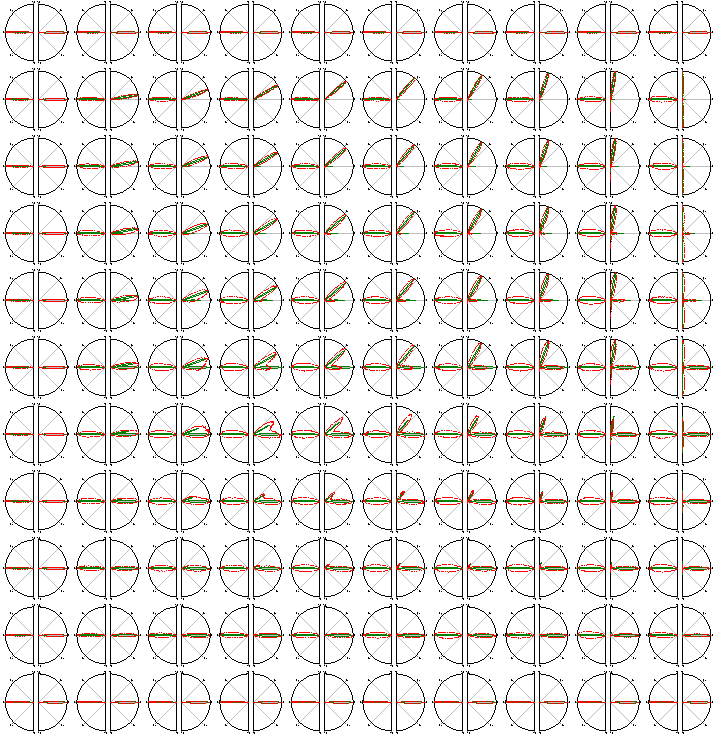
\includegraphics[width=1.0\textwidth]{gfx/model/results/model_analysis.pdf}};
% \begin{scope}[overlay]
%     \draw[->,thick] ($(image.north west)-(0.25,-0.25)$) -- ++(1,0) node [midway, above] {$\Omega$};
%     \draw[->,thick] ($(image.north west)-(0.25,-0.25)$) -- ++(0,-1) node [midway, above, rotate=90] {$\Psi$};
% \end{scope}
% \path ($(image.north west) + (-.5,.5)$) -- ($(image.north east) + (.5,.5)$);
% \end{tikzpicture}
% }
% \caption{model init vs solved}
% \label{app:model_histogram}
% \end{figure}
% %
% \begin{figure}[!tb]
% \centering
% \resizebox{1.0\textwidth}{!}{
% \begin{tikzpicture}[>=latex]
% \node[inner sep=0pt] (image) at (0,0)
%     {\includegraphics[width=1.0\textwidth]{gfx/model/results/histogram.pdf}};
% \begin{scope}[overlay]
%     \draw[->,thick] ($(image.north west)-(0.25,-0.25)$) -- ++(1,0) node [midway, above] {$\Omega$};
%     \draw[->,thick] ($(image.north west)-(0.25,-0.25)$) -- ++(0,-1) node [midway, above, rotate=90] {$\Psi$};
% \end{scope}
% \path ($(image.north west) + (-.5,.5)$) -- ($(image.north east) + (.5,.5)$);
% \end{tikzpicture}
% }
% \caption{Histogram cube\_2pop\_model}
% \label{app:model_histogram}
% \end{figure}
% %
% %
% \begin{figure}[!tb]
% \centering
% \resizebox{1.0\textwidth}{!}{
% \begin{tikzpicture}[>=latex]
% \node[inner sep=0pt] (image) at (0,0)
%     {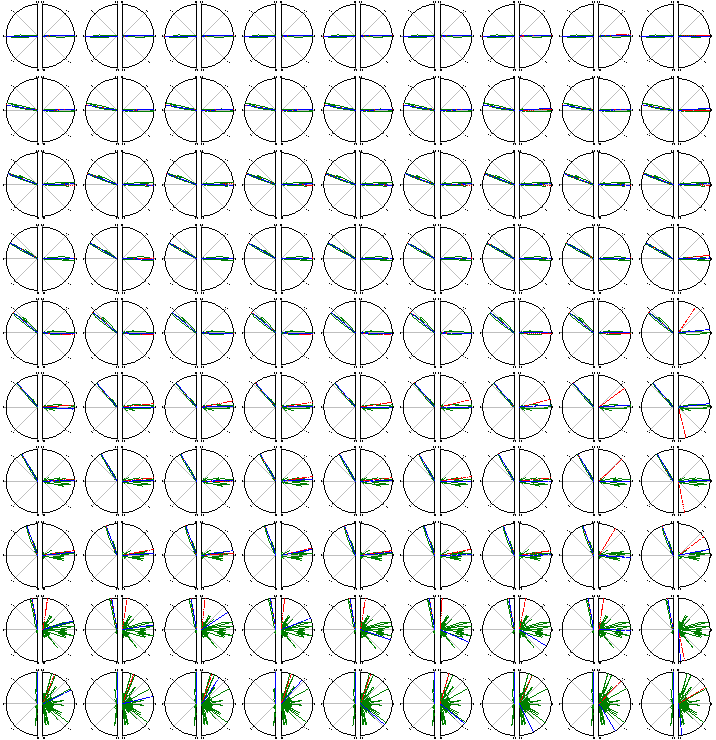
\includegraphics[width=1.0\textwidth]{gfx/model/results/voxel_size_simulation_analysis.pdf}};
% \begin{scope}[overlay]
%     \draw[->,thick] ($(image.north west)-(0.25,-0.25)$) -- ++(1,0) node [midway, above] {$voxel_size$};
%     \draw[->,thick] ($(image.north west)-(0.25,-0.25)$) -- ++(0,-1) node [midway, above, rotate=90] {$f0_inc$};
% \end{scope}
% \path ($(image.north west) + (-.5,.5)$) -- ($(image.north east) + (.5,.5)$);
% \end{tikzpicture}
% }
% \vspace{-1ex}
% \begin{center}
% \begin{tikzpicture}
%     \draw[thin] (-3.0,-0.625) rectangle (3.0,0.25);
%     \draw [green!50!black] (-2.5,0) -- (-1.5,0) node [below, midway, black] {truth};
%     \draw [red,dashed] (-0.5,0) -- (0.5,0) node [below, midway, black] {model=r};
%     \draw [blue, dash dot] (1.5,0) -- (2.5,0) node [below, midway, black] {model=p};
% \end{tikzpicture}
% \end{center}
% \caption{voxel\_size\_5\_}
% \label{app:model_histogram}
% \end{figure}
% %
% \begin{figure}[!tb]
% \centering
% \resizebox{1.0\textwidth}{!}{
% \begin{tikzpicture}[>=latex]
% \node[inner sep=0pt] (image) at (0,0)
%     {\includegraphics[width=1.0\textwidth]{gfx/simpli/results/simulation_analysis_spheres_LAP_p.pdf}};
% \begin{scope}[overlay]
%     \draw[->,thick] ($(image.north west)-(0.25,-0.25)$) -- ++(1,0) node [midway, above] {$\mathfrak{f}_0^\alpha$};
%     \draw[->,thick] ($(image.north west)-(0.25,-0.25)$) -- ++(0,-1) node [midway, above, rotate=90] {$\mathfrak{f}_0^\Psi$};
% \end{scope}
% \path ($(image.north west) + (-.5,.5)$) -- ($(image.north east) + (.5,.5)$);
% \end{tikzpicture}
% }
% \caption{Sphere LAP p}
% \label{app:model_histogram}
% \end{figure}
% %
% \begin{figure}[!tb]
% \centering
% \resizebox{1.0\textwidth}{!}{
% \begin{tikzpicture}[>=latex]
% \node[inner sep=0pt] (image) at (0,0)
%     {\includegraphics[width=1.0\textwidth]{gfx/simpli/results/simulation_analysis_spheres_LAP_r.pdf}};
% \begin{scope}[overlay]
%     \draw[->,thick] (image.north west) -- ++(1,0) node [midway, above] {$\alpha_0$};
%     \draw[->,thick] (image.north west) -- ++(0,-1) node [midway, above, rotate=90] {$\Psi_0$};
% \end{scope}
% \path ($(image.north west) + (-.5,.5)$) -- ($(image.north east) + (.5,.5)$);
% \end{tikzpicture}
% }
% \caption{Sphere LAP r}
% \label{app:model_histogram}
% \end{figure}
% %
% \begin{figure}[!tb]
% \centering
% \resizebox{1.0\textwidth}{!}{
% \begin{tikzpicture}[>=latex]
% \node[inner sep=0pt] (image) at (0,0)
%     {\includegraphics[width=1.0\textwidth]{gfx/simpli/results/simulation_analysis_spheres_PM_p.pdf}};
% \begin{scope}[overlay]
%     \draw[->,thick] ($(image.north west)-(0.25,-0.25)$) -- ++(1,0) node [midway, above] {$f_0$};
%     \draw[->,thick] ($(image.north west)-(0.25,-0.25)$) -- ++(0,-1) node [midway, above, rotate=90] {$\Psi$};
% \end{scope}
% \path ($(image.north west) + (-.5,.5)$) -- ($(image.north east) + (.5,.5)$);
% \end{tikzpicture}
% }
% \caption{Sphere PM p}
% \label{app:model_histogram}
% \end{figure}
% %
% \begin{figure}[!tb]
% \centering
% \resizebox{1.0\textwidth}{!}{
% \begin{tikzpicture}[>=latex]
% \node[inner sep=0pt] (image) at (0,0)
%     {\includegraphics[width=1.0\textwidth]{gfx/simpli/results/simulation_analysis_spheres_PM_r.pdf}};
% \begin{scope}[overlay]
%     \draw[->,thick] ($(image.north west)-(0.25,-0.25)$) -- ++(1,0) node [midway, above] {$f_0$};
%     \draw[->,thick] ($(image.north west)-(0.25,-0.25)$) -- ++(0,-1) node [midway, above, rotate=90] {$\Psi$};
% \end{scope}
% \path ($(image.north west) + (-.5,.5)$) -- ($(image.north east) + (.5,.5)$);
% \end{tikzpicture}
% }
% \caption{Sphere PM r}
% \label{app:model_histogram}
% \end{figure}
% %
% \begin{figure}[!t]
% \centering
% \resizebox{1.0\textwidth}{!}{
% \includegraphics[width=\textwidth, page=2]{dev/rc1/cube_2pop_orientation_hist2d_output_cube_2pop_135_rc1.pdf}
% }
% \caption[Model orientation histograms]{density distribution of fiber segment orientation in initial and resulting models for $\fiberRadius = \SI{1}{\micro\meter}$. \itodo{fit ESAG} \ITODO{these are only resulting models!}}
% \label{app:modelOrientation}
% \end{figure}
% %
% %
%
\chapter{} % Model analysis
\label{app:modelAnalysis}
%
%
\fakesection{Model parameter}
%
\begin{figure}[!h]
    \centering
    \includegraphics[width=1\textwidth]{dev/rc1/mpara/pre_stats_box_plot_volume_output_parameter_statistic_rc1.pdf}
    \caption{Caption}
    \label{app:appModelVolumeBoxPlot}
\end{figure}
%
% % \foreach \n in {1,3,...,10}{
% % \begin{landscape}
% \begin{figure}[!t]
% \centering
% % \resizebox{\textwidth}{!}{
% \includegraphics[width=\textwidth,page=1]{dev/rc1/mpara/pre_stats_time_evolve_all_output_parameter_statistic_rc1.pdf}
% \includegraphics[width=\textwidth,page=2]{dev/rc1/mpara/pre_stats_time_evolve_all_output_parameter_statistic_rc1.pdf}
% \end{figure}
% % \end{landscape}
%
%
\fakesection{Time evolution}
%
\setlength{\tikzwidth}{\textwidth}
\begin{sidewaysfigure}[]
\centering
\includegraphics[height=\tikzwidth,page=1]{dev/rc1/mpara/pre_stats_time_evolve_all_output_parameter_statistic_rc1.pdf}
\includegraphics[height=\tikzwidth,page=2]{dev/rc1/mpara/pre_stats_time_evolve_all_output_parameter_statistic_rc1.pdf}
\label{app:pste1}
\end{sidewaysfigure}
%
\begin{sidewaysfigure}[]
\centering
% \resizebox{\tikzwidth}{!}{
\includegraphics[height=\tikzwidth,page=3]{dev/rc1/mpara/pre_stats_time_evolve_all_output_parameter_statistic_rc1.pdf}
\includegraphics[height=\tikzwidth,page=4]{dev/rc1/mpara/pre_stats_time_evolve_all_output_parameter_statistic_rc1.pdf}
% }
\label{app:pste2}
\end{sidewaysfigure}
%
\begin{sidewaysfigure}[]
\centering
% \resizebox{\textwidth}{!}{
\includegraphics[height=\tikzwidth,page=5]{dev/rc1/mpara/pre_stats_time_evolve_all_output_parameter_statistic_rc1.pdf}
\includegraphics[height=\tikzwidth,page=6]{dev/rc1/mpara/pre_stats_time_evolve_all_output_parameter_statistic_rc1.pdf}
\label{app:pste3}
\end{sidewaysfigure}
%
\begin{sidewaysfigure}[]
\centering
% \resizebox{\textwidth}{!}{
\includegraphics[height=\tikzwidth,page=7]{dev/rc1/mpara/pre_stats_time_evolve_all_output_parameter_statistic_rc1.pdf}
\includegraphics[height=\tikzwidth,page=8]{dev/rc1/mpara/pre_stats_time_evolve_all_output_parameter_statistic_rc1.pdf}
\label{app:pste4}
\end{sidewaysfigure}
%
\begin{sidewaysfigure}[]
\centering
% \resizebox{\textwidth}{!}{
\includegraphics[height=\tikzwidth,page=9]{dev/rc1/mpara/pre_stats_time_evolve_all_output_parameter_statistic_rc1.pdf}
\includegraphics[height=\tikzwidth,page=10]{dev/rc1/mpara/pre_stats_time_evolve_all_output_parameter_statistic_rc1.pdf}
\label{app:pste5}
\end{sidewaysfigure}
%
%
\fakesection{Histogramms}
%
\begin{figure}
    \centering
    \includegraphics[width=\textwidth, page=2]{dev/rc1/cube_2pop_orientation_hist2d_output_cube_2pop_135_rc1.pdf}
    \caption{Caption}
    \label{app:modelHistOrientation}
\end{figure}[]
%
\fakesection{Speedup}
%
\begin{figure}[!t]
\centering
\includegraphics[page=2]{dev/rc1/speed/boxplot_output_r_0.5__.pkl_speedup.csv.pdf}
\caption[\code{model.Sovler} speedup]{\code{model.Sovler} speedup. The time measurements are taken after $\Delta_{\mathit{steps}}$ for the next $\SI{25}{\steps}$ for parallel $(||)$ and crossing $(\times)$ fiber configurations.}
\label{app:solverSpeedupAll}
\end{figure}
%
%
%
\fakesection{Simulation Library}
\begin{table}[htb]
\centering
\caption[Opening angle distribution]{Orientation statistic of simulation model library.}
\resizebox{\textwidth}{!}{
\pgfplotstabletypeset[%
    thesisTableStyle,
    columns={omega,psi,pop,incl_mean,incl_std,incl_25,incl_50,incl_75,phi_mean,phi_std,phi_25,phi_50,phi_75,mean,std,25,50,75},
    every head row/.style={
        before row={
            \toprule
        },
        after row={$\si{\degree}$ & & & $\si{\degree}$ & $\si{\degree}$ & $\si{\degree}$ & $\si{\degree}$ & $\si{\degree}$ & $\si{\degree}$ & $\si{\degree}$ & $\si{\degree}$ & $\si{\degree}$ & $\si{\degree}$ & $\si{\degree}$ & $\si{\degree}$ & $\si{\degree}$ & $\si{\degree}$ & $\si{\degree}$ \\ \midrule},
    },
    columns/omega/.style={column name=$\Omega$},
    columns/psi/.style={column name=$\Psi$},
    columns/mean/.style={column name=$<d\Omega>$,zerofill,precision=0},
    columns/std/.style={column name=$\sigma(d\Omega)$,zerofill,precision=0},
    columns/25/.style={column name=$25(d\Omega)$,zerofill,precision=0},
    columns/50/.style={column name=$50(d\Omega)$,zerofill,precision=0},
    columns/75/.style={column name=$75(d\Omega)$,zerofill,precision=0},
    columns/incl_mean/.style={column name=$<\alpha>$,fixed,fixed zerofill,precision=0},
    columns/incl_std/.style={column name=$\sigma(\alpha)$,fixed,fixed zerofill,precision=0},
    columns/incl_25/.style={column name=$25(\alpha)$,fixed,fixed zerofill,precision=0},
    columns/incl_50/.style={column name=$50(\alpha)$,fixed,fixed zerofill,precision=0},
    columns/incl_75/.style={column name=$75(\alpha)$,fixed,fixed zerofill,precision=0},
    columns/phi_mean/.style={column name=$<\varphi>$,fixed,fixed zerofill,precision=0},
    columns/phi_std/.style={column name=$\sigma(\varphi)$,fixed,fixed zerofill,precision=0},
    columns/phi_25/.style={column name=$25(\varphi)$,fixed,fixed zerofill,precision=0},
    columns/phi_50/.style={column name=$50(\varphi)$,fixed,fixed zerofill,precision=0},
    columns/phi_75/.style={column name=$75(\varphi)$,fixed,fixed zerofill,precision=0},
    col sep=comma,
    %
]
{dev/rc1/domega/omegas_ms_2pop.csv}
}
\label{app:modelDistribution}
\end{table}
%
% 
%
\chapter{}
\label{app:Simulation}
%
\fakesection{Tissue}
%
\begin{sidewaysfigure}[!p]
\resizebox{\textheight}{!}{
\begin{tabular}{cc}
\includegraphics[]{dev/rc1/tissue/bf_rc1_retardation_PM_Roden.pdf}&
\includegraphics[]{dev/rc1/tissue/bf_rc1_retardation_PM_Human.pdf}\\
\includegraphics[]{dev/rc1/tissue/bf_rc1_transmittance_PM_Roden.pdf}&
\includegraphics[]{dev/rc1/tissue/bf_rc1_transmittance_PM_Human.pdf}
\end{tabular}}
\end{sidewaysfigure}
%
\fakesection{Voxelsize}
%
\begin{figure}[!p]
% 2_simulation/0_parameter/fiber_radii.py
\centering
\includegraphics[width=\textwidth, page=1]{dev/rc1/voxel_size/voxel_size_plots_data_output_vs_135_0.01_6_25_vervet_r_rc1.pdf}
\caption[voxel size model with noise]{The mean difference is constant for smaller voxel sizes and does not start to grow significantly before $\voxels=\SI{0.125}{\micro\meter}$.}
\label{app:voxelsizeNoise}
\end{figure}
%
%
%
\fakesection{domega}
%
\begin{figure}[!t]
    \centering
    \includegraphics[]{dev/rc1/domega/cube_2pop_domega_analysis_all_output.pdf}
    \caption{Direction and inclination distribution of simulation model library.}
    % \label{fig:my_label}
\end{figure}
%
%
%
% %%%%%%%%%%%%%%%%%%%%%%%%%%%%%%%%%%%%%%%%%%%%%%%%%%%%%%%%%%%
% SINGLE
% %%%%%%%%%%%%%%%%%%%%%%%%%%%%%%%%%%%%%%%%%%%%%%%%%%%%%%%%%%%
%
\fakesection{Single fiber population}
%
\begin{figure}[!p]
\centering
% \begin{minipage}{0.45\textwidth}
\resizebox{\textwidth}{!}{
\rotatebox{90}{
\begin{tabular}{c|c}
\begin{tabular}{c|c}
    \includegraphics[]{dev/rc1/single/cube_2pop_135_rc1_single_plots_single_pop_hist_0.0.pdf} &
    \includegraphics[]{dev/rc1/single/cube_2pop_135_rc1_single_plots_single_pop_hist_25.0.pdf} \\
    \includegraphics[]{dev/rc1/single/cube_2pop_135_rc1_single_plots_single_pop_hist_5.0.pdf} &
    \includegraphics[]{dev/rc1/single/cube_2pop_135_rc1_single_plots_single_pop_hist_30.0.pdf} \\
    \includegraphics[]{dev/rc1/single/cube_2pop_135_rc1_single_plots_single_pop_hist_10.0.pdf} &
    \includegraphics[]{dev/rc1/single/cube_2pop_135_rc1_single_plots_single_pop_hist_35.0.pdf} \\
    \includegraphics[]{dev/rc1/single/cube_2pop_135_rc1_single_plots_single_pop_hist_15.0.pdf} &
    \includegraphics[]{dev/rc1/single/cube_2pop_135_rc1_single_plots_single_pop_hist_40.0.pdf} \\
    \includegraphics[]{dev/rc1/single/cube_2pop_135_rc1_single_plots_single_pop_hist_20.0.pdf} &
    \includegraphics[]{dev/rc1/single/cube_2pop_135_rc1_single_plots_single_pop_hist_45.0.pdf}
\end{tabular}
&
\begin{tabular}{c|c}
    \includegraphics[]{dev/rc1/single/cube_2pop_135_rc1_single_plots_single_pop_hist_50.0.pdf} &
    \includegraphics[]{dev/rc1/single/cube_2pop_135_rc1_single_plots_single_pop_hist_75.0.pdf} \\
    \includegraphics[]{dev/rc1/single/cube_2pop_135_rc1_single_plots_single_pop_hist_55.0.pdf} &
    \includegraphics[]{dev/rc1/single/cube_2pop_135_rc1_single_plots_single_pop_hist_80.0.pdf} \\
    \includegraphics[]{dev/rc1/single/cube_2pop_135_rc1_single_plots_single_pop_hist_60.0.pdf} &
    \includegraphics[]{dev/rc1/single/cube_2pop_135_rc1_single_plots_single_pop_hist_85.0.pdf} \\
    \includegraphics[]{dev/rc1/single/cube_2pop_135_rc1_single_plots_single_pop_hist_65.0.pdf} &
    \includegraphics[]{dev/rc1/single/cube_2pop_135_rc1_single_plots_single_pop_hist_90.0.pdf} \\
    \includegraphics[]{dev/rc1/single/cube_2pop_135_rc1_single_plots_single_pop_hist_70.0.pdf} &
\end{tabular}
\end{tabular}
}}
%
\caption[sim]{left: 2d log histogramm orientation from rofl analysis of simulation, right: 2d log histogramm of orientation of model segemnts. \itodo{rfc plots}}
\label{app:single_fiber_pop_hist_app}
\end{figure}
%
%
% %%%%%%%%%%%%%%%%%%%%%%%%%%%%%%%%%%%%%%%%%%%%%%%%%%%%%%%%%%%
% FLAT
% %%%%%%%%%%%%%%%%%%%%%%%%%%%%%%%%%%%%%%%%%%%%%%%%%%%%%%%%%%%
%
\fakesection{Crossing fiber population}
%
\begin{figure}[!p]
\centering
\setlength{\tikzwidth}{0.45\textwidth}
\begin{tabular}{c|c}
    \includegraphics[width=\tikzwidth]{dev/rc1/flat/cube_2pop_135_rc1_flat_plots_flat_pop_hist_omega_0.0_psi_0.3.pdf} &
    \includegraphics[width=\tikzwidth]{dev/rc1/flat/cube_2pop_135_rc1_flat_plots_flat_pop_hist_omega_50.0_psi_0.3.pdf} \\
    \includegraphics[width=\tikzwidth]{dev/rc1/flat/cube_2pop_135_rc1_flat_plots_flat_pop_hist_omega_10.0_psi_0.3.pdf} &
    \includegraphics[width=\tikzwidth]{dev/rc1/flat/cube_2pop_135_rc1_flat_plots_flat_pop_hist_omega_60.0_psi_0.3.pdf} \\
    \includegraphics[width=\tikzwidth]{dev/rc1/flat/cube_2pop_135_rc1_flat_plots_flat_pop_hist_omega_20.0_psi_0.3.pdf} &
    \includegraphics[width=\tikzwidth]{dev/rc1/flat/cube_2pop_135_rc1_flat_plots_flat_pop_hist_omega_70.0_psi_0.3.pdf} \\
    \includegraphics[width=\tikzwidth]{dev/rc1/flat/cube_2pop_135_rc1_flat_plots_flat_pop_hist_omega_30.0_psi_0.3.pdf} &
    \includegraphics[width=\tikzwidth]{dev/rc1/flat/cube_2pop_135_rc1_flat_plots_flat_pop_hist_omega_80.0_psi_0.3.pdf} \\
    \includegraphics[width=\tikzwidth]{dev/rc1/flat/cube_2pop_135_rc1_flat_plots_flat_pop_hist_omega_40.0_psi_0.3.pdf} &
    \includegraphics[width=\tikzwidth]{dev/rc1/flat/cube_2pop_135_rc1_flat_plots_flat_pop_hist_omega_90.0_psi_0.3.pdf}
\end{tabular}
%
\caption[sim]{psi=0.3; left: 2d log histogramm orientation from rofl analysis of simulation, right: 2d log histogram of orientation of model segemnts. \itodo{legende}}
\label{app:flat_03_fiber_pop_hist}
\end{figure}
%
%
%
%
\begin{figure}[!p]
\centering
\setlength{\tikzwidth}{0.45\textwidth}
\begin{tabular}{c|c}
    \includegraphics[width=\tikzwidth]{dev/rc1/flat/cube_2pop_135_rc1_flat_plots_flat_pop_hist_omega_0.0_psi_0.5.pdf} &
    \includegraphics[width=\tikzwidth]{dev/rc1/flat/cube_2pop_135_rc1_flat_plots_flat_pop_hist_omega_50.0_psi_0.5.pdf} \\
    \includegraphics[width=\tikzwidth]{dev/rc1/flat/cube_2pop_135_rc1_flat_plots_flat_pop_hist_omega_10.0_psi_0.5.pdf} &
    \includegraphics[width=\tikzwidth]{dev/rc1/flat/cube_2pop_135_rc1_flat_plots_flat_pop_hist_omega_60.0_psi_0.5.pdf} \\
    \includegraphics[width=\tikzwidth]{dev/rc1/flat/cube_2pop_135_rc1_flat_plots_flat_pop_hist_omega_20.0_psi_0.5.pdf} &
    \includegraphics[width=\tikzwidth]{dev/rc1/flat/cube_2pop_135_rc1_flat_plots_flat_pop_hist_omega_70.0_psi_0.5.pdf} \\
    \includegraphics[width=\tikzwidth]{dev/rc1/flat/cube_2pop_135_rc1_flat_plots_flat_pop_hist_omega_30.0_psi_0.5.pdf} &
    \includegraphics[width=\tikzwidth]{dev/rc1/flat/cube_2pop_135_rc1_flat_plots_flat_pop_hist_omega_80.0_psi_0.5.pdf} \\
    \includegraphics[width=\tikzwidth]{dev/rc1/flat/cube_2pop_135_rc1_flat_plots_flat_pop_hist_omega_40.0_psi_0.5.pdf} &
    \includegraphics[width=\tikzwidth]{dev/rc1/flat/cube_2pop_135_rc1_flat_plots_flat_pop_hist_omega_90.0_psi_0.5.pdf}
\end{tabular}
%
\caption[sim]{psi=0.5; left: 2d log histogramm orientation from rofl analysis of simulation, right: 2d log histogramm of orientation of model segemnts. \itodo{legende}}
\label{app:flat_05_fiber_pop_hist}
\end{figure}
%
%
%
\begin{figure}[!p]
\centering
\resizebox{\textwidth}{!}{
\begin{tabular}{cc}
\includegraphics[page=1]{dev/rc1/analysis/plots_flat_pop_output_cube_2pop_135_rc1_flat.pdf} &
\includegraphics[page=2]{dev/rc1/analysis/plots_flat_pop_output_cube_2pop_135_rc1_flat.pdf}\\
\includegraphics[page=3]{dev/rc1/analysis/plots_flat_pop_output_cube_2pop_135_rc1_flat.pdf} &
\includegraphics[page=4]{dev/rc1/analysis/plots_flat_pop_output_cube_2pop_135_rc1_flat.pdf}
\end{tabular}
}
\end{figure}
%
\begin{figure}[!p]
\centering
\resizebox{\textwidth}{!}{
\begin{tabular}{cc}
\includegraphics[page=5]{dev/rc1/analysis/plots_flat_pop_output_cube_2pop_135_rc1_flat.pdf} &
\includegraphics[page=6]{dev/rc1/analysis/plots_flat_pop_output_cube_2pop_135_rc1_flat.pdf}\\
\includegraphics[page=7]{dev/rc1/analysis/plots_flat_pop_output_cube_2pop_135_rc1_flat.pdf} &
\includegraphics[page=8]{dev/rc1/analysis/plots_flat_pop_output_cube_2pop_135_rc1_flat.pdf}
\end{tabular}
}
\end{figure}
%
\begin{figure}[]
\centering
\resizebox{\textwidth}{!}{
\begin{tabular}{cc}
\includegraphics[page=9]{dev/rc1/analysis/plots_flat_pop_output_cube_2pop_135_rc1_flat.pdf} &
\includegraphics[page=10]{dev/rc1/analysis/plots_flat_pop_output_cube_2pop_135_rc1_flat.pdf}
\end{tabular}
}
\end{figure}
%
%
% %%%%%%%%%%%%%%%%%%%%%%%%%%%%%%%%%%%%%%%%%%%%%%%%%%%%%%%%%%%
% INCLINED
% %%%%%%%%%%%%%%%%%%%%%%%%%%%%%%%%%%%%%%%%%%%%%%%%%%%%%%%%%%%
%
\fakesection{Inclined fiber population}
%
\begin{figure}[!p]
\centering
\setlength{\tikzwidth}{0.45\textwidth}
\begin{tabular}{c|c}
    \includegraphics[width=\tikzwidth]{dev/rc1/inclined/cube_2pop_135_rc1_inclined_plots_inclined_pop_hist_omega_0.0_psi_0.3.pdf} &
    \includegraphics[width=\tikzwidth]{dev/rc1/inclined/cube_2pop_135_rc1_inclined_plots_inclined_pop_hist_omega_50.0_psi_0.3.pdf} \\ \includegraphics[width=\tikzwidth]{dev/rc1/inclined/cube_2pop_135_rc1_inclined_plots_inclined_pop_hist_omega_10.0_psi_0.3.pdf} & \includegraphics[width=\tikzwidth]{dev/rc1/inclined/cube_2pop_135_rc1_inclined_plots_inclined_pop_hist_omega_60.0_psi_0.3.pdf} \\
    \includegraphics[width=\tikzwidth]{dev/rc1/inclined/cube_2pop_135_rc1_inclined_plots_inclined_pop_hist_omega_20.0_psi_0.3.pdf} &
    \includegraphics[width=\tikzwidth]{dev/rc1/inclined/cube_2pop_135_rc1_inclined_plots_inclined_pop_hist_omega_70.0_psi_0.3.pdf} \\ \includegraphics[width=\tikzwidth]{dev/rc1/inclined/cube_2pop_135_rc1_inclined_plots_inclined_pop_hist_omega_30.0_psi_0.3.pdf} & \includegraphics[width=\tikzwidth]{dev/rc1/inclined/cube_2pop_135_rc1_inclined_plots_inclined_pop_hist_omega_80.0_psi_0.3.pdf} \\
    \includegraphics[width=\tikzwidth]{dev/rc1/inclined/cube_2pop_135_rc1_inclined_plots_inclined_pop_hist_omega_40.0_psi_0.3.pdf} &
    \includegraphics[width=\tikzwidth]{dev/rc1/inclined/cube_2pop_135_rc1_inclined_plots_inclined_pop_hist_omega_90.0_psi_0.3.pdf}
\end{tabular}
%
\caption[sim]{psi=0.3; left: 2d log histogramm orientation from rofl analysis of simulation, right: 2d log histogram of orientation of model segemnts. \itodo{legende}}
\label{app:incl_03_fiber_pop_hist}
\end{figure}
%
%
%
%
\begin{figure}[!p]
\centering
\setlength{\tikzwidth}{0.45\textwidth}
\begin{tabular}{c|c}
    \includegraphics[width=\tikzwidth]{dev/rc1/inclined/cube_2pop_135_rc1_inclined_plots_inclined_pop_hist_omega_0.0_psi_0.5.pdf} &
    \includegraphics[width=\tikzwidth]{dev/rc1/inclined/cube_2pop_135_rc1_inclined_plots_inclined_pop_hist_omega_50.0_psi_0.5.pdf} \\
    \includegraphics[width=\tikzwidth]{dev/rc1/inclined/cube_2pop_135_rc1_inclined_plots_inclined_pop_hist_omega_10.0_psi_0.5.pdf} &
    \includegraphics[width=\tikzwidth]{dev/rc1/inclined/cube_2pop_135_rc1_inclined_plots_inclined_pop_hist_omega_60.0_psi_0.5.pdf} \\
    \includegraphics[width=\tikzwidth]{dev/rc1/inclined/cube_2pop_135_rc1_inclined_plots_inclined_pop_hist_omega_20.0_psi_0.5.pdf} &
    \includegraphics[width=\tikzwidth]{dev/rc1/inclined/cube_2pop_135_rc1_inclined_plots_inclined_pop_hist_omega_70.0_psi_0.5.pdf} \\
    \includegraphics[width=\tikzwidth]{dev/rc1/inclined/cube_2pop_135_rc1_inclined_plots_inclined_pop_hist_omega_30.0_psi_0.5.pdf} &
    \includegraphics[width=\tikzwidth]{dev/rc1/inclined/cube_2pop_135_rc1_inclined_plots_inclined_pop_hist_omega_80.0_psi_0.5.pdf} \\
    \includegraphics[width=\tikzwidth]{dev/rc1/inclined/cube_2pop_135_rc1_inclined_plots_inclined_pop_hist_omega_40.0_psi_0.5.pdf} &
    \includegraphics[width=\tikzwidth]{dev/rc1/inclined/cube_2pop_135_rc1_inclined_plots_inclined_pop_hist_omega_90.0_psi_0.5.pdf}
\end{tabular}
%
\caption[sim]{psi=0.5; left: 2d log histogramm orientation from rofl analysis of simulation, right: 2d log histogramm of orientation of model segemnts. \itodo{legende}}
\label{app:incl_05_fiber_pop_hist}
\end{figure}
%
%
%
\begin{figure}[!p]
\centering
\resizebox{\textwidth}{!}{
\begin{tabular}{cc}
\includegraphics[page=1]{dev/rc1/analysis/plots_inclined_pop_output_cube_2pop_135_rc1_inclined.pdf} &
\includegraphics[page=2]{dev/rc1/analysis/plots_inclined_pop_output_cube_2pop_135_rc1_inclined.pdf}\\
\includegraphics[page=3]{dev/rc1/analysis/plots_inclined_pop_output_cube_2pop_135_rc1_inclined.pdf} &
\includegraphics[page=4]{dev/rc1/analysis/plots_inclined_pop_output_cube_2pop_135_rc1_inclined.pdf}
\end{tabular}
}
\end{figure}
%
\begin{figure}[!p]
\centering
\resizebox{\textwidth}{!}{
\begin{tabular}{cc}
\includegraphics[page=5]{dev/rc1/analysis/plots_inclined_pop_output_cube_2pop_135_rc1_inclined.pdf} &
\includegraphics[page=6]{dev/rc1/analysis/plots_inclined_pop_output_cube_2pop_135_rc1_inclined.pdf}\\
\includegraphics[page=7]{dev/rc1/analysis/plots_inclined_pop_output_cube_2pop_135_rc1_inclined.pdf} &
\includegraphics[page=8]{dev/rc1/analysis/plots_inclined_pop_output_cube_2pop_135_rc1_inclined.pdf}
\end{tabular}
}
\end{figure}
%
\begin{figure}[!p]
\centering
\resizebox{\textwidth}{!}{
\begin{tabular}{cc}
\includegraphics[page=9]{dev/rc1/analysis/plots_inclined_pop_output_cube_2pop_135_rc1_inclined.pdf} &
\includegraphics[page=10]{dev/rc1/analysis/plots_inclined_pop_output_cube_2pop_135_rc1_inclined.pdf}
\end{tabular}
}
\end{figure}
%
% %
% %
%
% \newpage
% \mbox{}
%
% **************************************************
% End of Document CONTENT
% **************************************************
\end{document}
